\documentclass[11pt]{report}
\usepackage{appendix}
\usepackage{multicol}
\usepackage{titlesec}
\usepackage{nameref}
\newcommand{\hsp}{\hspace{20pt}}
\newcommand{\signbox}[1]{%
	\begin{tabular}{@{}p{0.35\linewidth}@{}}
		\\
		\\
		\\
		\\
		\hrule \\
		\centering #1
	\end{tabular}
}
\usepackage{pbox}
\usepackage[normalem]{ulem}
\usepackage{ifpdf}
\usepackage{listings}
\usepackage{color}
\definecolor{lightgray}{rgb}{.9,.9,.9}
\definecolor{darkgray}{rgb}{.4,.4,.4}
\definecolor{purple}{rgb}{0.65, 0.12, 0.82}
\definecolor{lightblue}{rgb}{0.65, 0.65, 1}
%\newpagestyle{main}{%
	%\titleformat{\chapter}[hang]{\Huge\bfseries\hfill}{\thechapter\hsp\color{lightblue}{\textbar}\hsp}{0pt}{\Huge\bfseries}[\titlerule]%
%}

\lstdefinelanguage{JavaScript}{
  keywords={typeof, new, true, false, catch, function, return, null, catch, switch, var, if, in, while, do, else, case, break},
  keywordstyle=\color{blue},
  ndkeywords={class, export, boolean, throw, implements, import, this},
  ndkeywordstyle=\color{darkgray}\bfseries,
  identifierstyle=\color{black},
  sensitive=false,
  comment=[l]{//},
  morecomment=[s]{/*}{*/},
  commentstyle=\color{purple}\ttfamily,
  stringstyle=\color{red}\ttfamily,
  morestring=[b]',
  morestring=[b]"
}

\lstset{
   language=JavaScript,
   backgroundcolor=\color{lightgray},
   extendedchars=true,
   basicstyle=\footnotesize\ttfamily,
   showstringspaces=false,
   showspaces=false,
   numbers=left,
   numberstyle=\footnotesize,
   numbersep=9pt,
   tabsize=2,
   breaklines=true,
   showtabs=false,
   captionpos=b
}
\newenvironment{tabulenum}{\vspace{-1em}\begin{enumerate}}{\end{enumerate}\vspace{-2em}}
\newenvironment{tabulitem}{\vspace{-1em}\begin{itemize}}{\end{itemize}\vspace{-1.5em}}
%\newcommand{\tabulenum}[1]{\vspace{-1em}\begin{enumerate}#1\end{enumerate}\vspace{-2em}}
\newcommand{\code}[1]{\texttt{#1}}
\newcommand{\specialcell}[2]{%
  \begin{tabular}{@{}p{#1}@{}}#2\end{tabular}}
\newcommand{\blankpage}{\newpage\thispagestyle{empty}\mbox{}}
\usepackage[utf8]{inputenc}
\usepackage{longtable,lscape}
\usepackage{rotating}
\usepackage[margin=0.75in]{geometry}
\usepackage{fancyhdr}
\usepackage{pdfpages}
\pagestyle{fancy}
\lhead{}
\ifpdf
   \PassOptionsToPackage{pdftex,usenames,dvipsnames}{graphicx}
   \usepackage[pdftex]{graphicx}   % to include graphics
    \pdfcompresslevel=9 
    \usepackage[pdftex,     % sets up hyperref to use pdftex driver
            plainpages=false,   % allows page i and 1 to exist in the same document
            breaklinks=true,    % link texts can be broken at the end of line
            colorlinks=false,
            pdftitle=My Document
            pdfauthor=My Good Self,
%            hidelinks=true
           ]{hyperref} 
    \usepackage{thumbpdf}
\else 
    \usepackage{graphicx}       % to include graphics
    \usepackage[hidelinks]{hyperref}       % to simplify the use of \href
\fi 
% \title{Development of a BLOPP prototype system for medication of children using Android and Karotz}
% \author{Esben Aarseth, \\
%   J\o rgen Aaberg, \\
%   Aleks Gisvold, \\
%   Eirik Skjeggestad Dale, \\  
%   Yngve Svalestuen
%   }
% \date{}
\begin{document}
\begin{titlepage}
	\begin{center}
		\includegraphics[height=7cm]{Pictures/Logo}\\[1cm]

		\textsc{\LARGE Norwegian University of Science and Technology}\\[1.5cm]

		\textsc{\Large TDT4290 --- Customer Driven Project}\\[0.2cm]
		\textsc{\Large Group 2}

		{\rule{\linewidth}{0.5mm}} \\[0.4cm]
		{\huge \bfseries BLOPP - Development of a prototype system for treatment of asthmatic children, using Android and Karotz}
		{\rule{\linewidth}{0.5mm}} \\[1.5cm]

		J{\o}rgen \textsc{Aaberg}\\
		Esben \textsc{Aarseth}\\
		Eirik Skjeggestad \textsc{Dale}\\
		Aleksander \textsc{Gisvold}\\
		Yngve \textsc{Svalestuen}

		\vfill

		{\large \today}

	\end{center}
\end{titlepage}
\blankpage{}
\section*{Abstract}
\setcounter{page}{1}
\pagenumbering{roman}
%This master-level course TDT4290 Customer Driven Project deals with a project assignment that is mandatory for all computer science students. 
%The purpose of this project is to teach students, by working in groups, software engineering skills in context of a development project. 
%The students are to make a realistic prototype of an Information System “on contract” for a real world customer.
% Hæ?

%Our Customer is NAAF (Norges Astma og Allergiforbund) and ``Sykehusapotekene i Norge''.  Contact information for both the customer and 
%the development team is listed in the Introduction Chapter.  

%The development team consists of Esben, Aleksander, Jørgen, Yngve and Eirik, all Computer Science students at NTNU.
% The students are taking this course as a part of their master degree in computer science.
% In very brief summary, our assignment and project goal was to create two applications in order to motivate both children and parents to 
% follow up a medicational plan. For the application made for children the purpose is to make a better and more fun way for the children 
% to take asthma-medication with use of mobile technology. For the application made for parents the purpose is to make it easier to learn 
% how to take medicine the right way, and follow up and log a medicational plan. 

This project aimed to create three applications to motivate and remind asthmatic children to 
take their medication. When children are on a medication plan, taking the medicine might be boring or stressful 
because they are reminded of their asthma, are disturbed in their routine, or that the medication
process itself is scary. The use of an appealing figure like the rabbit robot Karotz provides a way to avoid
some of these concerns. In combination with a reminder and distraction application and an adult information
and settings application, the complete system could help leviate the burden of medicating asthmatic children.

The three applications were developed on two different platforms. The guardian application for configuration, 
teaching and viewing a log, and a children application for teaching, reminding and distracting during treatment were developed 
for the Android platform. A second application for reminding and distracting the children during treatment was made for 
Karotz. Through the agile software development technique SCRUM, the project team completed five sprints of 
iterative study, planning, programming, adaption and testing. The Android applications are written in Java, 
while the Karotz application is written in JavaScript. A central database is written in MySQL 
with PHP sites for access through the internet protocol HTTP.

The prototype system is developed for Sykehusapotekene i Midt-Norge as a part of NTNU's course TDT4290 --- Customer Driven Project.

\paragraph{Keywords:}
\emph{BLOPP, Asthma, Gamification, Android, Karotz, SCRUM, Software development}
% dette er en fin abstract, men den er litt kort.
% TODO: beskrive litt mer rundt prosjektet: platformene (android + karotz), NTNU-faget (bittelitt på slutten, ingen navn)

\vfill
\noindent \signbox{J{\o}rgen Aaberg} \hfill \signbox{Esben Aarseth}
\signbox{Eirik Skjeggestad Dale} \hfill \signbox{Aleksander Gisvold}
\begin{center}\signbox{Yngve Svalestuen}\end{center}
\vspace*{4cm}
{\tableofcontents}
{\listoffigures}
{\listoftables}
%\pagestyle{main}
\chapter{Introduction}
\label{chap:intro}
\setcounter{page}{1}
\pagenumbering{arabic}
This chapter contains a brief introduction to the project and the layout of the 
report. It gives an overview of project goals, and the documentation of the development 
process. This introduction also explains the background for the given project and 
how the project's success is measured. 

In Section \ref{sec:prosec} we give details on the project, including project name, 
background, task, terms, planned effort and result schedule.

In Section \ref{sec:custinf} we give detailed customer information including
information on the sponsor, partners, customer contacts, project group, and
and overview of affiliates. The affiliates include a table of stakeholders.
  
% description of the project and the customer in Section x.x and x.x, a
% description of the project background is given in Section x.x and contains the
% reason for the project as well as the motivation behind such a project.  The
% stakeholders are identified and listed in Section x.x in order to clarify what
% parties are affecting and being affected by the project. A discussion of the
% effects of the project is given in Section x.x and the duration of the project
% is explained in Section x.x. Finally, there is a short outline of the rest of
% the report in section x.x.

\section{Project Information}
\label{sec:prosec}
\subsection{Project Name}
The name of this project is ``BLOPP", and was decided by the customer. BLOPP stands for ``Barns 
LegemiddelOPPlevelse'' (``Children's experience with medication'').  

\subsection{Background}

Many children today have to take inhalation medicines because of chronic or
acute lung disease such as asthma. Children often find it difficult to use
the medication correctly, boring or even scary to take them, which means they
might object or forget to take them. Parents also sometimes
apply the medication incorrectly, apply the wrong treatment, or even forget to
give the medication to their
children. This may lead to reduced effect of the medication, and the lung disease
may worsen and last longer, causing increased pressure on the public health
services, increased health related cost and lost working hours for the parents.




\subsection{The task}
Our task was to implement two Android applications, one application for the parents, Guardian Application (GAPP), 
and one application for children, Children Application (CAPP). In addition, an application for the Karotz platform 
should be created to assist and to an extent substitute the GAPP and CAPP mobile applications. 

The high level functional requirements for these applications are to be found in Table 
\ref{tab:highfuncitionalrequirements}. The functional requirements for all applications are described in more detail 
in Section \ref{sec:functionalRequirements}

\begin{table}
\centering
	\begin{tabular}{p{1.5cm}|p{12cm}}
		\hline
		\bf{\#} & \bf{Description} \\  \hline \\

		GHR1 & The application must alert the parent(s) when it is time for a medication/treatment for their child. \\ \\
		GHR2 & The application must log the health status of their child, according to section \ref{sec:trafficlight}. \\ \\ 
		GHR3 & The application should log pollen casts for the area the child is in, and which medications were taken each day.\\ \\ 
		GHR4 & The application must store medical plans for their child. These plans concern asthma medications, and contains which medicines should be taken at which times.\\ \\ 
		GHR5 & The application must provide instructions on how to use different medications. These instructions may be pictures or text, provided by NAAF. \\ \\ \hline \\

		CHR1 & The application should distract the children during a treatment. \\ \\ 
		CHR2 & The application should gamify their experience with medication.  \\ \\ \hline \\

		KHR1 & The application should alert children and parent(s) when it is time for a medication/treatment for the children.  \\ \\ 
		KHR2 & The application should distract the children during a treatment. \\ \\ 
		KHR3 & The application should encourage children to take medication through interactivity and gamification.  \\
		\hline
	\end{tabular}
	\caption[High level functional requirements]{High level functional requirements. GHR: GAPP requirement, CHR: CAPP requirement, KHR: karotz application requirement}
	\label{tab:highfuncitionalrequirements}
\end{table}
\clearpage{}

\subsection{Measurement of project effort}
The customer was seeking a documented prototype of a system which could be used for future 
development and for getting additional funding for further development of the project. The customer wanted
the prototype tested on children suffering from diseases causing breathing problems and their parents, in order
to determine whether or not such a system was an adequate solution to the problem. The system should be
compatible with Android v4.0 or newer versions, and should be intuitive to use. The resulting prototype should be well documented
to ensure that further development would be able to continue development after the end of the project.

\subsection{General terms}
We were to make two applications for Android devices and one for Karotz. Originally the customer wanted the smart phone applications made for iOS, 
but since we did not have Apple computers and iPhones, and the customer did not have the funding to provide them, we 
switched to the Android platform. We had at our disposal a Karotz robot with a yellow and a green Nanoz controller,
a Github repository, an AgileZen board and could request an Android tablet to be used for testing if necessary.

\subsection{Planned effort}
The course description states an expected effort of 25 hours per week per student. The course lasted for 13 weeks,
resulting in a total expected effort of 325 hours per student, at a total of 1625 for the team altogether.

\subsection{Schedule of results}
The applications were scheduled to be completed within November 10th. The time we had left after this, was used for fixing
critical errors, and completing the report.

\subsection{Report Outline}
The report is outlined in Table \ref{tab:chapters}. 

\begin{table}
	\begin{center}
	\begin{tabular}{|p{0.3\linewidth}|p{0.6\linewidth}|}   
		\hline   
		\bf{Chapter} & \bf{Description} \\ 
		\hline
			Chapter \ref{chap:intro}: \nameref{chap:intro} &
			 Contains a short description of the project, its goals and purpose and what the 
			 report consists of. \\
		\hline
			Chapter \ref{chap:projectManagement}: \nameref{chap:projectManagement} & 
			Contains a description of how the group is organized and what responsibilities 
			lies on each of the group members. A risk analysis for the project is also included
			 in this chapter, as well as the work plan which describes the different phases, 
			 activities and a Gantt Diagram for the project. Quality Assurance
			 techniques are also discussed, which include meetings, coding templates and document templates. \\
		\hline
			Chapter \ref{chap:prestudy}: \nameref{chap:prestudy} & 
			Contains a documentation of the preliminary studies done ahead of the implementation of the 
			applications, including a report of the design workshop done early in development,
			development methodology, frameworks and tools used in the project, the Karotz platform 
			and information about asthma. \\
		\hline
			Chapter \ref{chap:developmentMethodology}: \nameref{chap:developmentMethodology} &
			Contains description and discussion about the various development methods considered
			for the project, and an analysis of SCRUM, the chosen methodology. \\
		\hline
			Chapter \ref{chap:requrementSpecifications}: \nameref{chap:requrementSpecifications} &
			Contains an overview of the requirement specifications for the system, through use cases
			and functional requirements. \\
		\hline
			Chapter \ref{chap:systemDesign}: \nameref{chap:systemDesign} & 
			Contains a collection of requirements and design choices for the prototype, 
			including use cases, architectural description and documentation of the database. \\
		\hline
			Chapter \ref{chap:testPlan}: \nameref{chap:testPlan} & 
			Describes how the team will do testing throughout the project. \\
		\hline
			Chapter \ref{chap:sprint1}-\ref{chap:sprint5}: \nameref{chap:sprint1}-\nameref{chap:sprint5} & 
			Contains the goals, backlogs, test tables, results and reviews for the respective sprints. \\
		\hline
			Chapter \ref{sec:Usabilitytesting}: \nameref{sec:Usabilitytesting} &
			Contains a description of usability testing in general, and reports and discussion from the 
			usability tests done in the project.\\
		\hline
			Chapter \ref{chap:furtherWork}: \nameref{chap:furtherWork} & 
			Contains a description of what has been implemented and what the next logical steps 
			are based on the current state of the system. \\
		\hline
			Chapter \ref{chap:evaluation}: \nameref{chap:evaluation} & 
			Contains the evaluation and description of how the project was executed. \\
		\hline
	\end{tabular}
	\end{center}
	\caption{Chapters and their respective description}
	\label{tab:chapters}
\end{table}

\section{Customer Information}
\label{sec:custinf}
The customer of this project is "Sykehusapotekene i Midt-Norge". 

\subsection{Sponsor}
The sponsor of this project is Extrastiftelsen.

\subsection{Partners}
The Norwegian University of Technology and Science are partner in this project. Norges Astma og Allergiforbund (NAAF) has also been included in the work, both for feedback and helpful information. Table \ref{tab:customercontacts} shows relevant contacts for the customer. 

\subsection{Customer contacts}
Table \ref{tab:customercontacts} gives an overview of the contact information for the customers.
\begin{table}
	\begin{center}
		\begin{tabular}{|p{4cm}|p{7cm}|}   
			\hline      
			\bf{Name} & \bf{Email} \\ 
			\hline
			Ole Andreas Alsos & \href{mailto:oleanda@idi.ntnu.no}{oleanda@idi.ntnu.no}  \\     
			\hline
			Elin Høien & \href{mailto:elin@hoien.no}{elin@hoien.no}
			\\
			\hline
			Marikken Høiseth &
			\href{mailto:marikken.hoiseth@ntnu.no}{marikken.hoiseth@ntnu.no}\\
			\hline
			Hanne Linander &
			\href{mailto:hanne.linander@gmail.com}{hanne.linander@gmail.com}
			\\
			\hline
		 \end{tabular}
	\end{center}
	\caption{Customer contacts}
	\label{tab:customercontacts}
\end{table}
\clearpage{}
%Vi bør ta enten tabell, eller project group her. Tabellen må da selvsagt utvides.
\subsubsection{Project Group}
\begin{itemize}
  	\item Cand Pharm Elin Bergene, Sykehusapotekene i Midt-Norge (Hospital pharmacies in Central Norway)
	\item PhD Ole Andreas Alsos, Norsk Senter for Elektronisk Pasientjournal (NSEP) (Norwegian Center for Electronic Patient Journal) and Institute for Computer Science (IDI), NTNU (Ph.D as of 2011). Ole is also working part time at BEKK Consulting. 
	\item Scholarship Marikken Høiseth, Institute for Product Design (IPD), NTNU.
	\item Bo Alexander Gleditsch, communication advisor NAAF.
	\item Rose Lyngra, senior advisor NAAF.
\end{itemize}

\subsubsection{Affiliates}
The project is in close collaboration with the following affiliates:
\begin{itemize}
  	\item Sykehusapotekene i Midt-Norge (SHAP) will be a test arena for the result of the project. They will work further with the results.
	\item Norsk Senter for Elektronisk Pasientjournal (NSEP). NTNUs activities within health informatics is gathered at NSEP. The project will take advantage of 
the academic community and the infrastructure at NSEP (offices and usability lab).
	\item Department for product design (IPD) at NTNU will consult upon design. 
	\item Department for computer and information science arranges the course and will provide an advisor for the group, Tobias B. Iversen. 
	\item Norges Astma og AllergiForbund (NAAF). The project has been created by NAAF. NAAF will provide expertise about the user groups of the final applications. NAAF will work further with the results of the project. 
\end{itemize}

\subsubsection{Stakeholders}
A stakeholder is a person, group or an organization that has interest in a project. The
different stakeholders of this project are listed in Table \ref{tab:stakeholders}. This table also contains
a short rationale for why each party has been listed, and what their main
concerns for the applications are.

\begin{table}
	\begin{center}
		\begin{tabular}{|p{0.3\linewidth}|p{0.6\linewidth}|}   
			\hline      
			\bf{Stakeholder} & \bf{Rationale} \\ 
			\hline
			NAAF & Wants to see whether this is a possible solution to make it easier for children to take their medicine. Also interested in proof-of-concept.
			\\
			\hline
			Sykehusapotekene i Midt-Norge & Cooperates with NAAF to find out if there is an easier
			way to make children take their medicine. 
			\\
			\hline
			Developers & Wants the applications to be a success, as it is their work. The level of success also affects the degree in one of their courses.
			\\
			\hline
			NTNU & Wants the project to be a success to front the research that is done by
			the university.
			\\
			\hline
			Children diagnosed with asthma & Needs something to make it easier to go through
			with each treatment.
			\\
			\hline
			Parents of children diagnosed with asthma & Needs instructions on how to use
			medicines correctly. Needs reminders about when to give their children their medicines. Needs an
			organized way to see what medicines have been taken earlier. Wants their children to
			suffer less during medication, and be happier about taking their medicine.
			\\
			\hline 
			Extrastiftelsen & Main funder of the project. 
			\\
			\hline
		\end{tabular}
	\end{center}
	\caption{Stakeholders}
	\label{tab:stakeholders}
\end{table}
\chapter{Project Management}
\label{chap:projectManagement}

\begin{table}[t]
	\begin{center}
		\begin{tabular}{|p{4cm}|p{7cm}|p{4cm}|}   
			\hline      
			\bf{Name} & \bf{Email} & \bf{Phone number} \\ 
			\hline
			Esben Aarseth & \href{mailto:esbena@stud.ntnu.no}{esbena@stud.ntnu.no} & 48062321   \\     
			\hline
			Aleksander Gisvold & \href{mailto:aleksg@stud.ntnu.no}{aleksg@stud.ntnu.no}
			& 46692443 \\
			\hline
			Jørgen Aaberg & \href{mailto:jorgeaab@stud.ntnu.no}{jorgeaab@stud.ntnu.no} &
			98866209 \\
			\hline
			Eirik Skjeggestad Dale & \href{mailto:eiriksd@stud.ntnu.no}{eiriksd@stud.ntnu.no}
			& 90138539\\
			\hline
			Yngve Svalestuen & \href{mailto:yngvesva@stud.ntnu.no}{yngvesva@stud.ntnu.no} & 99101640 \\
			\hline
		\end{tabular}
		\caption[Members of developer team]{Members of developer team}
		\label{tab:members}
	\end{center}
\end{table}

\section{Members}
Table \ref{tab:members} shows an overview of the names, email addresses and phone numbers
for the members of the developer team.


%\section{Qualities among members}

We have summarized our technical qualities in the following table. Each team member has
evaluated themself.
\begin{table}[h]
\begin{center}
\begin{tabular}{|p{1.2cm}|p{1.3cm}|p{1.6cm}|p{0.9cm}|p{1.3cm}|p{1.4cm}|p{2cm}|p{1.4cm}|p{2cm}|}
\hline
\bf{Name} & \bf{Java} & \bf{Database} & \bf{\LaTeX} & \bf{Scrum} & \bf{GUI} &
\bf{Management} & \bf{Testing} & \bf{Architecture} \\
\hline
\bf{Aleks} & Medium & Low & Low & High &	High &	Medium & Low &	Medium \\
\hline \bf{Esben} & Medium & Medium & Low	& Medium & High	& Medium & Low	& High
\\
\hline \bf{Jørgen} & Medium & Low & Low & Low & High &	Medium & Medium & Medium
\\
\hline \bf{Eirik} & High & Low & Low & Low	& Medium	& Medium	& Medium	& High \\
\hline \bf{Yngve} & High & Low &	Low & Medium & Medium & Low & Medium & Medium
\\
\hline

\end{tabular}
\end{center}
\end{table}


\section{Roles}
Early in the planning phase, on August 24th 2012, the group held a meeting to distribute
team roles for the project. We discussed which parts were needed for a system fitting the description,
and we decided on four main parts: GUI, back-end, database and Karotz. In addition, proper development
requires testing so we saw the need for a person in charge of testing, and a person in charge of
general quality assurance. We also needed a high-level system architect who could keep the
project well-structured and easily maintainable, especially considering that the system spans over
at least three different subsystems (database, Karotz and Android applications). Since the group was to keep
close contact with both the customer and the group advisor, responsibilities were assigned to these
roles as well. There would also be a need to write reports for meetings with these third parties, so
a secretary was necessary. At last, the group had already decided to use an agile 
development model, so a person in charge of this was needed as well (``Scrum master").

We have identified the following roles for the project. 
\begin{itemize}
\item Test Master - Eirik
\item Scrum Master - Aleksander
\item Customer Contact - Aleksander
\item Advisor Contact - Esben
\item Document Owner - Yngve
\item Secretary - Jørgen
\item Karotz Developer - Yngve
\item Database Manager - Yngve
\item System Architect - Esben
\item Quality Assurance manager - Jørgen 
\end{itemize}


\section{Responsibilities among roles}

In the following section all roles and their responsibilities are explained.

\begin{description}
	\item[Test Master] The test master is responsible for developing a test plan, initiate testing 
		and follow up on test results. The test master will have the last vote in 
		whether a test is passed or not. The test master will be responsible for making sure all 
		parts of testing is done, including unit testing, integration testing, system 
		testing and acceptance testing with the customer.
	
	\item[Scrum Master] Scrum master is accountable for removing impediments to the ability of the team 
		to deliver the sprint goal. The scrum master is no team leader, but is a kind 
		of buffer between the development team and distracting influences. The scrum master 
		is responsible for ensuring that the scrum process is 
		used as intended.

	\item[Customer Contact] The customer contact is responsible of all contact with the customer outside 
		of the customer meetings. This includes sending meeting invitations, clarifying 
		questions outside of customer meetings and other inquiries to the customer. 
		The customer contact works as a single-point two-way communicator, to reduce 
		amount of communication points. 

	\item[Advisor Contact] The advisor contact is responsible of all contact with the advisor outside 
		of the advisor meetings. Including sending meeting invitations, clarifying 
		questions outside of advisor meetings and other inquiries to the advisor. Advisor 
		contact works as a single-point two-way communicator, to reduce amount of 
		communication points.

	\item[Document Owner] The Document owner is responsible of finding a suitable tool for writing the report 
		in \LaTeX, and finding solutions with problems regarding \LaTeX. The document owner is also responsible for making sure all the correct 
		documents is added to the report, and will let the group know if something is missing. 

	\item[Secretary]
		Secretary is responsible for taking notes during all internal, 
		customer and advisor meetings. Meeting reports should meet a specific standard, 
		given by the project compendium. It is the responsibility of the meeting 
		report master to ensure this standard is followed.

	\item[Karotz Developer]
		The robot bunny, named Karotz, has an API for implementing features for controlling 
		the robot with an application. 
		The Karotz developer is responsible for developing the Karotz specific part of the system. 

	\item[Database manager]
		The database manager is responsible for selecting a suitable database tool for 
		the applications. The role also includes the responsibility of managing the 
		database architecture and connections towards the database.

	\item[System architect]
		The system architect is responsible of the overall architecture of the source code. 
		The architect has final vote in decisions regarding architecture specific problems. 

	\item[Quality assurance manager]
		The quality assurance manager has the overall responsibility for the applications and reports quality.

\end{description}


\section{Weekly schedule}

The development team had the following fixed weekly schedule:

\begin{itemize}
\item Customer meeting: Monday 12:15-13:00
\item Advisor meeting: Monday 13:15-14:00
\end{itemize}
Rooms were reserved on demand. There were also at least one day a week were the development team works together in the same room. 

\section{Work Plan}
\label{sec:workplan}

\subsection{Phases}

\subsubsection{Planning phase}
In this phase, a lot of time went to researching development methodology,
different useful technologies (like \LaTeX{}, different frameworks, customer
needs, etc.), and deciding upon a template for the software architecture. This phase was scheduled 
for completion by September 16th. 

\subsubsection{Development}
This phase started as soon as the planning phase was completed and
approved by the customer. It included development of the different
applications and testing continuously. This phase was scheduled for completion by
November 15th.

\subsubsection{Report Writing}
This phase included writing the necessary documentation of the final code. A lot of work
was put into writing the report during the development phase. However, as the
report would be large, and we would need the time to make corrections
and add content. This phase was scheduled for completion by November 20th. 

\subsubsection{Planning of presentation}
Planning of the presentation was started after this report was completed. This phase was scheduled
for completion the day before the actual presentation November 22nd. 

\subsection{Activities}
\label{sec:activities}
We identified some big tasks that needed to be done during the project lifetime. These
tasks were essential to make the project a success. 

The identified tasks are:
\begin{itemize}
  \item Workshop
  \item Usability tests
  \item Integration tests
  \item Export applications and wrap up the source code
  \item Project presentation
  \item Final report correction
\end{itemize}

\subsection{Person-hours per activity and phase}
We planned the following person hours per phase. These numbers are based on the estimated project
effort according to the class staff, and how long we thought each phase would take. As the activities identified
in Section \ref{sec:activities} are activities ``baked into'' the different sprints during development, we have not included estimation for these 
(for instance, it is hard to know so early how many usability tests we need). Also, we would write the report continuously, 
and this is considered a subtask of both development and planning. For each sprint we planned to use 175 hours on development.
%TODO: begrunne 175 timer?
\begin{itemize}
  \item Development: 875 hours
  \item Planning: 425 hours
  \item Meetings: 125 hours
  \item Report completion: 30 hours
  \item Presentation planning: 30 hours
\end{itemize}

\subsection{Gantt Diagram}
Figure \ref{fig:gantt} shows the Gantt Diagram for the whole project period.
%TODO: write something about the gantt diagram
\begin{figure}
	\centering
		\includegraphics[width = 17.5 cm]{Pictures/ArchPictures/Gantt.png}
	\caption{Gantt project overview}
	\label{fig:gantt}
\end{figure}
\section{Risk Analysis}
This section contains the risk analysis we did before the project was started. The 
analysis helped the team detect the most relevant risks for the project, in order 
to be prepared if such a problem should occur. This allowed the team to make some preemptive 
measures as well as draw up strategies for handling a number of possible situations. 
In addition to a listing of internal and external risks, this section contains a SWOT 
analysis for a deeper understanding of the different relations in the project, both internal and external.

\subsection{Internal Risks}
Table \ref{tab:internalRisks} contains issues that the group identified as possible 
internal risks for the project.

\subsection{External Risks}
Table \ref{tab:externalRisks} contains issues that the group identified as possible external 
risks to the project.

\begin{table}
	\centering
		\begin{sideways}
			\begin{tabular}{|  c 	 |	l 	| 	p{4.0cm} 	 |	p{4.0cm} 	  |	c 	 |	p{4.0cm} 	| 	l| }
			\hline
			  \# & Activity 	& Risk factor 	& Consequences 	& Prob.& Strategy and action 							& Responsible \\
			\hline
			  IR1 & All		& Longterm illness among the development team.  	& M -- Decrease of productivity. Lack of expertise.	& M 	& Share information online. The ill developer keeps himself updated. 	& All \\
			\hline
			  IR2 & All		& Long-term leave. A group member takes a long-term leave.  & M -- Reduced capacity.  & L	&  Plan what the member shall do before he is leaving.		& The Member \\
			\hline
			  IR3 & All		& Internal conflicts among the developer team.		& M -- Bad mood. Less work effort.  & H	&  Bring it up, and handle it right away. Use the advisor. 		& All \\
			\hline
			  IR4 & All		& Deadlines not being reached.			 	& H -- Unfinished work.  & M	&  Predict work load and set project boundaries. 	& Project leader \\
			\hline
			  IR5 & All		& Group members busy with other courses.		 & L -- Reduced capacity & H	&  Common Google Calendar to plan meetings. The member finds another time to do the work. 	& All \\
			\hline
			  IR6 & All		& Group members leaves project.		 	& H -- Reduced capacity & L	&  Reduce the project boundaries.	& All \\
			\hline
			  IR7 & Meetings		& Group members showing up late.	 	& L -- Reduced capacity & H	&  The group member works more next time. Penalties. 	& All \\
			\hline
			  IR8 & Implementation		& Lack of knowledge or abilities.	 	& L -- More time goes to getting knowledge. & M & Getting the knowledge. 	& All \\
			  \hline
			\end{tabular}
		\end{sideways}
	\caption{Internal Risks}
	\label{tab:internalRisks}
\end{table}

\begin{table}
	\centering
		\begin{sideways}
			\begin{tabular}{|  c 	|	p{2.0cm} 	 |	p{4.0cm} 	 |	p{4.0cm} 	  |	c 	 |	p{4.0cm} 	| 	p{2.0cm}| }
				\hline
				  \# & Activity 	& Risk factor 	& Consequences 	& Prob.& Strategy and action 							& Responsible \\
				\hline
				  ER1 & All		& External conflicts. One or more of the group members is in conflict with the customer or the group advisor & M -- May lead to bad communication, lack of feedback etc. & L 	& Bring it up and handle it right away. If customer contact is in a really bad conflict, change customer contact.	& All \\
				\hline
				  ER2 & Design and implementation	& Customer changes requirements. The customer is very decisive and demanding. & H -- May stress the developers and and make them confused on what to prioritize.  & H	&  Force the customer to prioritize tasks. Compromise possible solutions. 	& Development team and customer \\
				\hline
				  ER3 & All		& There is insufficient input from the customer regarding the development process.  & M -- May lead to expectancies not being met.  & L &  Force input from customer.	& Development team and customer \\
				\hline
				  ER4 & Development	& Tools fail. Software tools stop working or are outdated. 	& M -- Development process halted.  & L	&  Do other work. For instance report writing, testing and refactoring. Find other solutions to the problem. & All \\
				\hline
				  ER5 & Development & Loss of data. Data connected to the project is lost, or is unavailable for a period of time.   & H -- Development put back in time. & L &  Prioritize tasks according to remaining time. 	& All \\
				\hline
				  ER6 & Meetings, Feedback	& One of the customers takes a long-term leave. & L -- May delay feedback, input and access to resources. & L & Require more from the other customer contacts. 	& The customer \\
				\hline
				  ER7 & Development & Cannot get the Karotz API to work. & H -- May lead to removal of this feature for the prototype. & L	&  Focus on other parts of the applications.  & Development team \\
				\hline
				  ER8 & Development		& Database not working at all.  & H -- May lead to hardcoding of all features for the prototype. & L & Hardcode necessary parts.	& Development team \\
				\hline
				  ER9 & Development		& Android devices stop working  & L -- May delay development since emulator has low performance. & L & The group member must switch to emulator. 	& Group member \\
				  \hline
			\end{tabular}
		\end{sideways}
	\caption{External Risks}
	\label{tab:externalRisks}
\end{table}

\subsection{SWOT analysis}
The following section contains an analysis of strengths, weaknesses, opportunities and threats 
to the project. The analysis is used as a strategic planning method which analyses the internal 
and external factors in a group. The internal factors are strengths and weaknesses while 
opportunities and threats represent the external factors. 

According to Jackson et. al (2002)\cite{swot}, the SWOT analysis' intended use is to get an overview of the internal and external factors at the 
beginning of the project. Later, the analysis was used to map which parts of the project 
should be relied upon the most, and which opportunities and strengths can help the progress of 
the project the most.
 
Keeping the high-risk parts of the project under close watch helped the team catch problems 
before they evolved. In cases where a diversion was required, the SWOT analysis supported the 
team.
%TODO update references

\subsubsection{Strengths}
Communication and knowledge were the two greatest strengths in the project group. The fact that all 
team members spoke Norwegian as their native language, and were fairly competent in English, made 
all communication and reporting easier. Deciding to do the reporting and programming in English, 
while all other means of communication in Norwegian led to fewer misunderstandings and made 
it easier to help each other out when problems occurred. Discussions were also more valuable 
since everyone were able to participate without the fear of missing out due to lack of understand 
foreign languages.
 
When it comes to the level of knowledge, all group members were fourth year Computer Science students. 
This implied that even though the group members were taking different paths as to which 
specialization they were following for their masters degree, they all had a common background. 
It was therefore to be expected that everyone could participate in both coding and writing. The 
consequences of somebody falling ill were low, since they could be replaced by another member of 
the team. 

The technology was being shared between all team members and every team member took part in each part of the development. 
In addition to the basic knowledge, team members have chosen their own combination of courses. 
This made the team more capable of solving a broad array of tasks and finding good solutions to problems. 
Another strength in the group was that everyone had experience from previous projects, some more 
than others, but everyone had been involved in IT related projects. This provided the team with 
the experience needed to avoid some common pitfalls and get a decent start on the projects. 
The applications is to be used by patients with chronic illnesses, such as asthma. Since there are 
members of the group with asthma, the group found it easier to take the end users situation into account.


\subsubsection{Weaknesses}
The team chose to use the document markup language \LaTeX, even though none of the members 
had used it before. This led to some problems during the start of the reporting. The team 
was able to find many different guidelines, research and tutorials to use \LaTeX, which made 
it a lot easier to use, but it took time to learn and configure everything. 
For most people, money is a huge motivating factor. Since this is a university course, 
the entire group worked for free, making a product someone else may profit from. 
This meant that the developers had to find some other form of motivation. 
The group is also given a single grade, based on the overall achievements and results made 
by the team as one unit. This resulted in the biggest possible gains being experience, 
knowledge, relations to customers and the final grade. As students, the grade is usually the 
most motivating factor we get from a course. With a common grade for the group, there is a 
risk that expectations for the final grade might differ among the team members, and that 
some members will settle for a lower grade than others. It could prove difficult to get 
everyone working equally hard and as a result, some group members might become frustrated. 
The team attempted to fight this risk factor by introducing this weakness and discussing what 
each member wanted to gain from the project.

\subsubsection{Opportunities}
The gamification concept behind BLOPP has a lot of potential users. There is a 
significant need for a technological breakthrough in the area of applications regarding
medication and motivation.

There exists many different applications for making medication plans, reminding 
users, logging intake of mediation and similar functionality. A search on Google Play, 
the application store for Android devices, with the search term ``Asthma" gives a result of 214 
applications. We downloaded a few of the free ones, and all where very targeted towards 
adult users, giving information, offering tracking logs and similar. 

NAAF is an organization with impact on political decisions regarding health care in 
Norway. As exemplified by the Norwegian law ``Diskriminerings- og 
tilgjengelighetsloven''\cite{diskrimineringsloven} (Discrimination and availability law), 
their work is often referred to in legislative bills and they are considered a very 
professional and respected organization. The fact that they are backing this project may 
give the project media attention\footnote{See Appendix \ref{apx:ArticleAdressa}}.

NAAF and the BLOPP-project wants to make an application targeting children, but in order 
to avoid spending money on a poor solution, BLOPP did this as a low-cost project 
first. Should this project result in a success, NAAF can apply for a financial support 
from the Department of Health to develop the project further. The concept may also be 
useful for children with other diseases that require scheduled medication. R{\o}d et al. 
(2006)\cite{helsebibastma} writes that 10-12\% of the Norwegian school children have asthma, 
which gives a potentially huge user group. 

The final application may also be easily rewritten and target persons with other 
diseases. This may be done without writing all code from the beginning, but rather 
change out the parts regarding what medicines are implemented in the solution. This will 
again give a very huge potential user group, since all people with need to take a 
medicine regularly may be a target user.

\subsubsection{Threats}
When making a new product, it is not always clear what the product is going to solve and 
how it is going to do it. Neither are the opportunities and the limitations. Therefore 
it is very likely that the product and requirements are going to change during the 
development process. It is critical that the team makes room for unexpected changes and 
that adapting to changes is made easy. 

To manage this risk, a good working relationship with the customer is necessary. Product tests 
and demonstrations need to be done iteratively with both users and customers. Failing to 
do this will be a huge threat to the project and therefore, communication and 
collaboration will be important. 
\section{Quality Assurance}
\label{sec:qualityAssurance}
\subsection{Language}
As a main language for the development project, Norwegian was chosen. 
The decision was due to all members, customer contacts and the advisor 
being Norwegian. The report is written in English. All code, including comments were all in English. The language in the applications was chosen
to be Norwegian, since the applications is targeted towards norwegian 
children who do not necessarily understand English.

\subsection{Customer Meeting}
Customer meetings were held once a week. The reason behind this schedule 
was due to the customers desire of high involvement in the project, and 
the belief that having a high frequency of meetings would result in a higher 
quality result. High involvement makes the process of feedback and new ideas 
easier, and restricts the possibilities for the development team tracking 
off course. The meetings were usually held on Mondays. If any unexpected 
events resulted in meetings being moved, a notice where given at least 24 hours in advance. 
The first customer meeting was held at St. Olavs Hospital the 21st of August. 

\subsection{Advisor Meeting}
%TODO update references
The advisor meeting were held each Monday at Campus Gl\o shaugen. See Appendix \ref{apx:templates} 
for a typical meeting agenda. The main items of the agenda was the meeting approval of the report from the last 
meeting, a project status report and discussion on problems and difficulties. 
A plan for the following week was also presented. During the meetings, the 
advisor was able give feedback on the status of the report regarding the 
quality expected from the final result. 



\blankpage{}
\chapter{Preliminary Studies}
\label{chap:prestudy}
\section{Children with asthma}
%%%%%%%%%%%%%%%%%%%%%%%%%%%%%%%%%%%%%%%%%%%%%%%%%%%%%%%%%%%%%%%%%%%%%%%%%%%%%%%%%Hva med en seksjon først generelt om astma, medisiner og medisineringsmetoder. Så mer direkte mot barn og astma. Og så la neste seksjon komme med problemene dette medfører (slik det er nå).
%%%%%%%%%%%%%%%%%%%%%%%%%%%%%%%%%%%%%%%%%%%%%%%%%%%%%%%%%%%%%%%%%%%%%%%%%%%%%%%%%
Asthma is a chronic inflamatory disease that affects the airways and lungs.\cite{naafastma} It is often more prominent in children, who are more 
active and easily excited than adults. The asthma is typically triggered by excitement, physical activity, rashes or allergies. The problem is 
managed by multiple medicines, 
with different schedules as to when to take them, and how much to take, depending on the condition of the child. There are inhalation medicines that 
consists of either small dust particles that effect the lungs locally, or saltwater that are inhaled as vapor, either alone or combined with other 
medicines to loosen up slime. Among these inhalation medicines is Ventoline and Flutide, seen in figure \ref{fig:ventoline} and \ref{fig:flutide}. 
There are also pills and liquid medicines that either affects the immune system or affects the body globally, not just locally in the lungs.

\begin{figure}
	\begin{minipage}[b]{0.4\linewidth}
		\centering
			\includegraphics[width=0.15\paperwidth]{Pictures/ventoline}
		\caption[Ventoline]{Ventoline\cite{ventoline} is an inhalation medicine that opens up the airways shortly after inhaling it.}
		\label{fig:ventoline}
	\end{minipage}
	\hspace{3cm}
	\begin{minipage}[b]{0.4\linewidth}
		\centering
			\includegraphics[width=0.15\paperwidth]{Pictures/flutide}
		\caption[Flutide]{Flutide is a steroid keeping the illness checked, but it has no immediate effect.}
		\label{fig:flutide}
	\end{minipage}
\end{figure}

The medicines can also be divided into medicines that have immediate effects, and are used during an asthma attack, while other medicines are preventative, 
and is taken on a regular schedule. These preventative medicines are targeted at bolstering your immune system before going to certain areas, or days
where the child is likely to be in contact with materials it is allergic to.	

With some of the inhalation medicines it's difficult to time the inhalation with the release of medicine, and here an inhalation chamber, or inhalation 
mask, is used. When the child has taken the nebulizer this way, usually once or twice a day, they must remember to wash their mouth afterwards.

Figure \ref{fig:paperprototype} shows an image of a nebulizer machine. The nebulizer machines often makes alot of noise, and can 
be scary to children. The nebulizer treatment takes between 2-10 minutes, 1-4 times a day.

\begin{figure}[t]
	\center
		\includegraphics[width=0.4\linewidth]{Pictures/nebulizer}
	\caption[A Nebulizer machine]{A nebulizer machine.\cite{nebulizer}}
	\label{fig:paperprototype}
\end{figure}

\subsection{Traffic Light Classification of Asthma Condition}
\label{sec:trafficlight}

The traffic light program is a way of classifying condition and resulting medication for asthmatic 
patients. It is a very simple system that requires very little knowledge to understand, and is 
therefore well-suited for a project aimed at children. The basic outline can be compared to a traffic
light.

Borge et al. (2002)\cite{livingwithasthma} defines the zones as \emph{green}, \emph{orange}, and \emph{red}
and describes effects and treatment for each of them.

\subsubsection{Green Zone}
Green is the normal zone. A patient in the green zone can be described as in ``regular condition''. 
He or she is breathing normally, even when doing light physical exercise.

When an asthmatic is the green zone, it is normal to take two to three different medicines each day,
often with cortisone

\subsubsection{Yellow Zone}
Yellow is the ``ill'' zone. When a patient is in the yellow zone, they exhibit moderate signs of illness
such as breathlessness and coughing. There may also be allergy reactions, and waking up at night from
breathlessness and coughing. A patient may be defined as being in the yellow zone if he or she has a cold.

In the yellow zone, patients typically take more medication than in the green zone. A normal amount
is 4 to 6 doses daily. The medication from the green plan is taken as normal, in addition to any new
medicines introduced by the yellow state.

\subsubsection{Red Zone}
The red zone is labeled the ``stop'' zone. A patient in the red zone will have almost closed airways,
making it very difficult to breathe and the person will have to stop any activities.

A patient in the red zone has to fix his or her state immediately. This could be by opening windows,
finding a good resting position, taking specific emergency medication or using specific breathing
techniques. If these courses of action don't help, the patient should immediately call the doctor. 

\section{Parents with children affected by asthma}

Parents of children with asthma face a series of challenges concerning the medication of their children. 
One of these challenges is to give the correct amount of medicine, the right type of medicine, at the 
correct time of the day. Many parents have experienced stressful mornings where they are late for work, 
their children are unwilling to take their medicine and they either do it in an incorrect manner, reducing the 
medicines effect, or not giving it at all. The medication plans can be hard to understand, even though they are 
designed to be easy, and it's typically only one of the parents that have been given the instructions from 
the doctor directly, making it even harder for the other one to do it correctly.

The children are not always happy about taking their medicine. The inhalation mask might be scary, the 
medication might interfere with their planned activities that day, or any number of other reasons the child 
might not want to take his/her medicine that day. Having to force a child to take their medicine could make the 
child associate taking the medicine with a negative experience, and it becomes increasingly difficult to 
give the medicine to the child. 

\section{The concept of gamification}

Gamification is the concept of applying game-design thinking to non-game applications to make them more fun 
and engaging. Nick Pelling (2011)\cite{pellingblog} writes that the term \emph{gamification} was introduced
in 2002, but was not popular before 2010 (Daniels, 2010\cite{danielsblog}).

Common techniques applied to introduce gamification to a process include, but are not limited to:
\begin{itemize}
  \item Achievements/badges
  \item Levels
  \item Leaderboards
  \item Progress bars
  \item Avatars
  \item Gifting
  \item Challenges
  \item Embedding of minigames
\end{itemize}

These techniques are all widely used. Here are some examples:
% footnote / bibliography alle
\begin{itemize}
  \item In games for platforms like Playstation and Xbox, gamification is frequently used
   to make people finish campaigns.(Hamari et.al, 2011\cite{trophies}) Trophies and achievements are used to motivate people to complete games 100\%. 
   You may have to collect every single item in the game, fight every boss and so on.
  \item Nike+ introduced gamification to training. (Zichermann et. al, 2011\cite{gamificationByDesign}) You can track how fast you run, your maximum pulse and so on, 
  and try to beat this target the next time you are running.
  \item You can ``check in'' to places you have been with Google Maps, Facebook, Foursquare, Google+, GoWalla, and similar applications.  
  \item Airline companies uses bonus points as motivation for customers to fly more with a company. (Gamification Wiki, 2012\cite{freqflyer}) At a certain 
  level of these points, you may get one more flight for free, get a free upgrade to a better seat and so on. 
\end{itemize} 

%Kanskje skrive om dette?
We hope gamification will help making children's treatment as enjoyable as possible. Michael 
Wu has proven that gamification has an impact on human motivation. Wu presents: ``Game 
mechanics and game dynamics are able to positively influence human behavior 
because they are designed to drive the players above the activation threshold (i.e. the upper 
right of the ability-motivation axis), and then trigger them into specific actions'' (Wu, 2011)\cite{gamification101}.  

The gamification elements most suited for children, is gifting and embedding of minigames. The gifting needs to be visual, and
the two elements can be interwoven to increase the effect, where the minigames changes according to what gifts you've already
achieved. Another way that can implement gifting targeted at children, is to implement a currency system, for example coins, and reward them
with physical rewards when they reach a certain amount of coins. The rewards could be all from small toys and candy, to larger items, depending
on the amount of coins, and the tasks performed to get the coins. A point here is to make sure the currency is very visual, to make sure even
young children understand how many coins they have.
The implementation of minigames would help greatly in distracting children during tedious tasks like nebulization treatments.

Gamification has a lot of positive sides, but it may have bad sides if gamification is done the wrong way.
The fact that we are using gamification to motivate children, makes this an even more serious concern. If children feel that
they are stuck in a game, motivation may very easily be broken down. So whatever concept we come up with, it has to be 
to motivate the children at all time. They cannot feel stuck with our app. This concept is up to the customer to create, 
while we will be implementing it.  

As written above, gamification may have negative effects on users. Anderson-Rainie (2012)\cite{andersonrainie} show results
that users are likely to not be motivated or feel that they are manipulated into completing a task. The 
research also show that users are likely to feel that gamification is too childish, and that gamification 
is a trend that will disappear within a few years. 

\section{Karotz}
Karotz.com (2012)\cite{karotz} describes Karotz as a robot shaped 
as a bunny that can interact with
a user through light, ear movement and sound. It can also take
input through a button, moving its ears, an RFID (Radio-frequency identification) chip, voice
commands and serial (Internet) communication.

The project includes developing an application for the Karotz
platform that will serve as an addition to the mobile applications.
It is therefore necessary to study its interfaces, development
methods and API of the machine.

\begin{figure}[h]
	\centering
		\includegraphics[height=10cm]{Pictures/karotzimg}
	\caption{Karotz: A bunny-shaped robot}
	\label{fig:karotz}
\end{figure}

\subsection{Application Platform}
Karotz application (called ``Appz'') are installed through an
online platform located on the Karotz web site. They can be
launched on the Karotz itself either through a scheduler, voice
commands or an RFID chip. These RFID chips come in various shapes,
sizes and colors. Figure \ref{fig:flatnanoz} and Figure 
\ref{fig:nanoztag} show examples of the different kinds of ``nanoz'',
that are small figures with an integrated RFID chip.

\begin{figure}
	\begin{minipage}[b]{0.4\linewidth}
		\centering
			\includegraphics[width=0.30\paperwidth]{Pictures/FlatnanozYellow}
		\caption[Flatnanoz]{A flat nanoz--flatnanoz-- a figure with an RFID chip used to provide input to a Karotz.}
		\label{fig:flatnanoz}
	\end{minipage}
	\hspace{3cm}
	\begin{minipage}[b]{0.4\linewidth}
		\centering
			\includegraphics[width=0.30\paperwidth]{Pictures/NanoztagGreen}
		\caption[Nanoztag]{A round nanoz--nanoztag-- a figure with an RFID chip used to provide input to a Karotz.}
		\label{fig:nanoztag}
	\end{minipage}
\end{figure}

Some mentionable applications made by other developers are 
``At Home'', an application that may register that someone checks 
in at the Karotz, and send an e-mail to a predetermined mail 
address, so children may tell their parents that they are home. 
``Twitter for Karotz'' may read you tweets and post tweets based 
on voice-commands. Another mention is ``Weather'' which may tell 
you the forecast for the day or the following day. It seems all 
applications registered at the Karotz website are fairly simple 
and have little functionality.

As for launching the BLOPP application, the times for the scheduler must
be manually set through the Karotz web site, so it cannot be 
used for notifications directly. The best option for the BLOPP 
implementation would therefore be to set a scheduler to start
every day at 00:00 and stop every day at 23:59. This way it can
be ensured that the application is always running, updating
itself with medications, status and times, and a timer can be
used to schedule notifications.

%\subsection{The two APIs}
The Karotz can be programmed in two different ways: either
through a web REST (Representational State Transfe) framework, 
or with JavaScript that runs as an embedded program on the robot itself.

The requirement that a REST program would have to be hosted
somewhere, combined with the fact that an embedded program 
provides more flexibility in terms of local storage to limit the
amount of information sent over a network makes the JavaScript
framework a more suitable choice for the BLOPP project.

%\subsection{Karotz Output Channels}
The Karotz has a few ways of providing output to the end-user. It
can be asked to
\begin{itemize}
    \item play sound files;
    \item move its ears;
    \item speak, using a TTS (text-to-speach) engine;
    \item illuminate its stomach in different colors;
    and
    \item communicate over the internet with HTTP (Hyper Text Transfer Protocol) GET and POST 
          methods.
\end{itemize}

For providing user commands, TTS could be an option if the engine
supported Norwegian, but since the language options are limited to
English, French, German and Spanish, speech will have to be
created by recording sound files and playing them with the
multimedia engine.

\section{Pollen forecast}
\label{sec:pollencast}
NAAF\cite{naafasthma} states that asthma- and pollen treatment needs to be seen in correlation.
Children may feel worse during pollen season than the rest of the year. We intend to give parents more analyzing tools by being able to see
connections between asthma symptoms and different types of pollen by using pollen data. It may occur that asthma is not the original source of 
a child's condition, but an allergy against a certain pollen is the source.  
NAAF hosts a pollen forecast at \url{http://pollenvarslingen.no/} which we intend to use. We have been given a user key for this cast, even though
they do not normally distribute this sort of information to application developers.
\section{Design workshop}
\label{sec:designWorkshop}
Before the first sprint, a design workshop was held. Hanne Linander, a
master student in Industrial Design at NTNU was responsible for the workshop.
The goal was to come up with different ideas for functionality and design, and
make an early sketch for the layout of the application.

At this stage in the study, we had not yet decided to develop two separate
applications, so we created layout suggestions for an application aimed to do
both tasks for children and for adults.

Many different exercises were completed throughout the day, in order to make as many
creative ideas as possible. Examples of exercises are short time boxed sketch
sessions, cross-collaboration without explaining thoughts behind the sketches,
different idea-competitions, among others. At the end the ideas were evaluated,
resulting in many discards and some being taken into further development.
After the workshop the sketches and the ideas were presented to the customer.
The development team was very happy about the results and decided to develop a
paperprototype from the sketches.

\subsection{Results}
We drew several sketches of how we envisioned the different views in an 
imagined Android application. 

Figure \ref{fig:dwMainMenu} shows a suggestion for the main menu in the 
application, where the action of taking medicine is in focus. The menu includes:
\begin{itemize}
  \item a log button where an adult can view medication history for the child,
  \item a manual button for learning how to use medication,
  \item a settings button for adjusting mediation schedule, alarm ringtone etc.,
  \item an ``about the app'' button for learning how to use the application,
  \item a display where one can view the current health state for the child, and
  		also click on it to change the health state, and
  \item a count of how many stars the child has collected, with the option to
  		click on that count to see more detailed information about the rewards
  		collected.
\end{itemize}

Figure \ref{fig:dwHealthState} illustrates how a user would see the health state
view separately from the menu. It would consist of three elements represented as
colored smileys; one for each health state. The healthy smiley would be green and
smiling, the sick one would be yellow and in a mellow mood, while the very sick
state would be represented by a red, frowning smiley. The currently active health
state could be displayed by illuminating the respective smiley, and clicking on
another would change the active state.

Figure \ref{fig:dwHealthStatePopup} shows how the health state view could be 
integrated into the main menu better by injecting it into an overlay. This could
make navigating the app more intuitive.

Figure \ref{fig:dwMediationView} is an image of the view a user would first see
when clicking the big ``medicine'' button in the main menu, or the view he or she
sees when redirected from a notification. It shows an image of the medicine to be
taken, and gives the option to go directly to the medication process through
clicking on the medicine image itself. If a user is unsure about how to use the
medication, there is illustrated an option where one would directly be brought to
the manual page for that medicine.

Figure \ref{fig:dwPickChild} shows a view one would be brought to if more than one
child was registered in one application. It shows an icon for each child and the
child's name. Clicking one one or the other would bring the user to the distraction
page for that child.

Figure \ref{fig:dwMediationViewCloudsThunderstorm} is an image of the first part of
the distraction animation a child would see. It shows dark clouds and a thunderstorm
that represents the child's state before taking medication. It was thought of as a 
way to motivate children to take medication in order to clear up the clouds, and as
something children could relate to by comparing their progress to the clouds.

Figure \ref{fig:dwMediationViewEmergingMedicine} is also part of the distraction
animation. It shows a medicine unit emerging from behind the clouds which are clearing
up while the medication is ongoing. The emerging medication was supposed to symbolize
the goodness of medication, while the clearing of clouds would symbolize the child's
lungs and airways clearing up.

Figure \ref{fig:dwChildRewardsView} illustrates how a child could view his or her
collected stars. There is a big star with a count next to it, which would show the 
total amount of stars. In addition, there is a scrolling view on the top where each
day would have an amount of stars on it, corresponding to how many stars the child had
received on that day. Lastly, there is an appealing figure on the page, in this case
a ``ninja master'', which would be an avatar for the child. It was imagined as
something that the child would purchase or obtain after reaching a certain amount of stars,
and the object itself would vary, serving as an additional motivational factor to
supplement the stars themselves.

Figure \ref{fig:dwAdultLogView} is a view where adults could check the progress and
medication history for a child. It would display graphs of condition and how good they
were at following a medication plan. Days would be colored after what condition the 
child was in on that day. The amount of stars the child collected is also shown in each
day, and a percentage of how often a given medicine is taken on the planned time is
displayed on the bottom right.

\begin{figure}
	\begin{minipage}[b]{0.46\linewidth}
		\centering
			\includegraphics[width=0.34\paperwidth]{Pictures/DesignWorkshop/MobileMainMenu}
		\caption[Main menu view from design workshop]{View for the main menu of the application.}
		\label{fig:dwMainMenu}
	\end{minipage}
	\hspace{1cm}
	\begin{minipage}[b]{0.46\linewidth}
		\centering
		\includegraphics[width=0.34\paperwidth]{Pictures/DesignWorkshop/HealthStateView}
	\caption[Change health state view from design workshop]{View for changing health state (active medication plan).}
	\label{fig:dwHealthState}
	\end{minipage}
\end{figure}

% \begin{figure}
% 	\begin{center}
% 		\includegraphics[width=7cm]{}
% 		\caption{View for the main menu of the application.}
% 		\label{fig:dwMainMenu}
% 	\end{center}
% \end{figure}

% \begin{figure}
% 	\begin{center}
% 		\includegraphics[width=7cm]{Pictures/DesignWorkshop/HealthStateView}
% 		\caption{View for changing health state (active medication plan).}
% 		\label{fig:dwHealthState}
% 	\end{center}
% \end{figure}

\begin{figure}
	\begin{minipage}[b]{0.46\linewidth}
		\centering
			\includegraphics[width=0.34\paperwidth]{Pictures/DesignWorkshop/HealthStateViewPopup}
		\caption[Change health state as pop up from design workshop]{View for changing health state as a pop up from the main menu.}
		\label{fig:dwHealthStatePopup}
	\end{minipage}
	\hspace{1cm}
	\begin{minipage}[b]{0.46\linewidth}
		\centering
		\includegraphics[width=0.34\paperwidth]{Pictures/DesignWorkshop/MedicationView}
	\caption[Start medication view from design workshop]{View for starting a medication and distraction process.}
	\label{fig:dwMediationView}
	\end{minipage}
\end{figure}

% \begin{figure}
% 	\begin{center}
% 		\includegraphics[width=7cm]{Pictures/DesignWorkshop/HealthStateViewPopup}
% 		\caption{View for changing health state as a popup from the main menu.}
% 		\label{fig:dwHealthStatePopup}
% 	\end{center}
% \end{figure}
% 
% \begin{figure}
% 	\begin{center}
% 		\includegraphics[width=7cm]{Pictures/DesignWorkshop/MedicationView}
% 		\caption{View for starting a medication and distraction process.}
% 		\label{fig:dwMediationView}
% 	\end{center}
% \end{figure}

\begin{figure}
	\begin{minipage}[b]{0.46\linewidth}
		\centering
			\includegraphics[width=0.34\paperwidth]{Pictures/DesignWorkshop/MedicationViewPickChild}
		\caption[Pick child view from design workshop]{View for choosing child to medicate at the start of medication mode.}
		\label{fig:dwPickChild}
	\end{minipage}
	\hspace{1cm}
	\begin{minipage}[b]{0.46\linewidth}
		\centering
		\includegraphics[width=0.34\paperwidth]{Pictures/DesignWorkshop/MedicationViewCloudsThunderstorm}
	\caption[Distraction view from design workshop]{Initial view of a distraction. Heavy clouds and thunderstorms represent the child's state before taking medicine.}
	\label{fig:dwMediationViewCloudsThunderstorm}
	\end{minipage}
\end{figure}

% \begin{figure}
% 	\begin{center}
% 		\includegraphics[width=7cm]{Pictures/DesignWorkshop/MedicationViewPickChild}
% 		\caption{View for choosing child to medicate at the start of medication mode.}
% 		\label{fig:dwPickChild}
% 	\end{center}
% \end{figure}
% 
% \begin{figure}
% 	\begin{center}
% 		\includegraphics[width=7cm]{Pictures/DesignWorkshop/MedicationViewCloudsThunderstorm}
% 		\caption{Initial view of a distraction. Heavy clouds and thunderstorms represent the child's state before taking medicine.}
% 		\label{fig:dwMediationViewCloudsThunderstorm}
% 	\end{center}
% \end{figure}

\begin{figure}
	\begin{minipage}[b]{0.46\linewidth}
		\centering
			\includegraphics[width=0.34\paperwidth]{Pictures/DesignWorkshop/MedicationViewEmergingMedicine}
		\caption[Distraction view 2 from design workshop]{Subsequent view of a distraction process. The medication is emerging while the clouds are disappearing, to symbolize the healing effects of medicine.}
		\label{fig:dwMediationViewEmergingMedicine}
	\end{minipage}
	\hspace{1cm}
	\begin{minipage}[b]{0.46\linewidth}
		\centering
		\includegraphics[width=0.34\paperwidth]{Pictures/DesignWorkshop/ChildRewardsView}
	\caption[Rewards view from design workshop]{View where children can view their collected reward (stars), and an acquired rank (in this case ``ninja master'').}
	\label{fig:dwChildRewardsView}
	\end{minipage}
\end{figure}

% \begin{figure}
% 	\begin{center}
% 		\includegraphics[width=7cm]{Pictures/DesignWorkshop/MedicationViewEmergingMedicine}
% 		\caption{Subsequent view of a distraction process. The medication is emergin while the clouds are disapeparing, to symbolize the healing effects of medicine.}
% 		\label{fig:dwMediationViewEmergingMedicine}
% 	\end{center}
% \end{figure}
% 
% \begin{figure}
% 	\begin{center}
% 		\includegraphics[width=7cm]{Pictures/DesignWorkshop/ChildRewardsView}
% 		\caption{View where children can view their collected reward (stars), and an acquired rank (in this case ``ninja master'').}
% 		\label{fig:dwChildRewardsView}
% 	\end{center}
% \end{figure}

\begin{figure}
	\begin{center}
		\includegraphics[width=7cm]{Pictures/DesignWorkshop/AdultLogView}
		\caption[Log view from design workshop]{View where adults can view the medication and health state history for a child.}
		\label{fig:dwAdultLogView}
	\end{center}
\end{figure}
\clearpage{}
\subsection{What was used in the further development}
Several ideas from the design workshop was used later in the development. We realized that we did not have sufficient time to make a very complicated distraction and
reward system for CAPP, so we decided to keep the ideas from the workshop about rewarding the child with stars whenever he or she completed a treatment.
This is easily implementable, and we believed it would be easy for parents to build on it with physical rewards when the child had accumulated enough stars.
For the same reasons we chose to keep and build on the idea of having an animation sequence where a Karotz avatar mirrored what the child had to do, it would
equip the inhalation mask when the child had to, making it more exciting for the child to do this as well. This approach have been seen to work with other applications,
like for helping children brush their teeth, and we wanted to use this as our base point.

We did the workshop based on the idea of having
one application, but later decided on having two. This meant that most of the basic GUI elements we came up with here, had
to be redone. For GAPP we implemented a log which kept its general layout, with the coloring showing which plan had been followed the relevant day. We later switched around on the additional information
that would be shown on each date and how, but the concept stayed the same.
\section{Frameworks used in the Project}
\label{sec:frameworks}
In this section the different frameworks that have been in use in the project is presented.
The frameworks consists mainly of the development model, the different programming languages, the 
database and server tools, the Karotz API, the Android SDK and the IDE used for development.


\subsection{Programming Languages, Message Formats and File Formats}
The following section will comment on different programming languages, communication protocols and 
file formats used in the project.

\subsubsection{Eclipse IDE}
\label{sec:Eclipse}
Eclipse \cite{Eclipse} is a multi-language software development environment comprising an integrated development environment (IDE) and an extensible plug-in system. The source code is mostly written in Java. Eclipse may be used to develop applications in Java and, by means of various plug-ins, other programming languages including Ada, C, C++, Ruby, Python, and many others. Eclipse is owned by the Eclipse Foundation, a non-profit organization focusing on creating and maintaining a community for individuals and organizations who wish to collaborate on commercially-friendly open source software. 

\subsubsection{Java}

Java is a programming language developed by Sun Microsystems in 1995, and is licensed under the GNU General Public License. 
Java can be run on any Java Virtual Machine (JVM), which means that it can run on any platform. It is an object oriented language and is based upon classes.
According to TIOBE Software (2012)\cite{TIOBE}, it was ranked as the 2nd most popular programming language in the world.


\subsubsection{Android SDK}
The Android software development kit (SDK) \cite{AndroidSDK} includes a comprehensive set of development tools used when developing Android software. The kit includes an Emulator, documentation of the source code, sample code, tutorials and a debugger. Enhancements to Android's SDK go hand in hand with the overall Android platform development. The SDK will also support older versions of the Android platform, through downloading extra packages of source code, in case developers wish to target their application towards older devices. By building the project through the IDE the Android application is packaged in a format which may be distributed (.apk). 

\subsubsection{Android Developer Tools}
The Android Developer Tools (ADT) \cite{AndroidADT} is a plug in for Eclipse that provides a professional-grade development environment for building Android applications. The ADT makes it easier to use the functions and tools that the Android SDK provides, by giving access through the user interface of Eclipse.


\subsubsection{Javadoc}
Javadoc is a tool for documenting code. It is integrated in Eclipse IDE, and we will use it document our code. When we use code-completion in Eclipse, the Javadoc of the function selected is shown as it's description.  

\subsubsection{JavaScript}
Two parts of the project will make use of JavaScript. The settings page for doctors is web based and 
will use JavaScript for interactivity. The Karotz can be programmed in two ways; either through a web 
API on the server side or through stored JavaScript code. In order to maximize stability and power, 
the client hosted JavaScript technique will be used.

JavaScript is a multi-paradigm, weakly typed and dynamic language that is extensively used on the web 
today. The main application of JavaScript is to enhance interactivity on a web page through client-side 
interpretation of the code in a browser. It can be used for a number of purposes such as making something 
happen when a button is pressed, loading new data without refreshing the page and much more. Even 
though JavaScript is by far most commonly used on the web there are also applications of it in other 
areas. Examples of these kinds of implementations are Node.js\cite{nodejs}, a network application creation
platform for writing JavaScript code as a regular server-side program, and the Karotz API which we will be 
using.

\subsubsection{Karotz API}
The Karotz API is based on a Javascript engine. The API is downloadable from the 
Karotz's homepage and gives access to the Karotz's different functions such as changing the color 
of the LED light, playing prerecorded sounds, waving it's ears and registering contact with an RFID-chip. 

A full documentation of the API is given, however most of the example code is commented in French.

\subsection{Database}
Since the project team has decided to use a database to store information relevant to the systems, there
is a requirement to use a programming language for creating and maintaining, as well as accessing, the
database. Because of technical limitations in the Karotz explained further in Section \ref{sec:databaseAccessLayer}
we chose to split the database into to parts: the database itself, written and maintained in MySQL, and
a set of access modules written in PHP (PHP: Hypertext Preprocessor) and MySQL.

\subsubsection{MySQL and phpMyAdmin}
MySQL\cite{mysql} is the world's leading open source database. It offers all the tools necessary to implement
and maintain data records for a project such as ours. The advantage of being the biggest contender is that there
is a myriad of resources easily and freely available to MySQL developers on the Internet. MySQL is suitable
for our project because it is reliable, free and open source, and all the group members have previous experience
working with it.

PhpMyAdmin is a graphical MySQL manager that is installed on NTNU's MySQL server\cite{ntnuphpmyadmin}. It provides
an easy way to manipulate a MySQL database without having to write any SQL code. Figure \ref{fig:phpmyadmin} shows
a typical screen from phpMyAdmin, where one can edit, add rows, add information etc. directly within a GUI. Since
NTNU's servers are already integrated with the program, and we use NTNU's MySQL server for development,
phpMyAdmin will be used to administer the database efficiently.

\begin{figure}
	\begin{center}
		\includegraphics[width=17.5cm]{Pictures/Tools/PhpMyAdmin}
	\end{center}
	\caption{phpMyAdmin screenshot}
	\label{fig:phpmyadmin}
\end{figure}

\subsubsection{PHP}
PHP\cite{php} is a scripting language that is extensively used on the web because of its flexibility, ease of use
and popularity. It is mainly used for creating and editing HTML (HyperText Markup Language) pages server-side before sending to the client. In
our project, we used PHP to access the NTNU MySQL database from a web server located on a NTNU sub network(\url{http://folk.ntnu.no/}), 
and return a JSON file.

\subsubsection{JSON}
JSON\cite{json} is a format used for storing and sending data in a light, human-readable and easily parsable format.
It's based on JavaScript notation, but uses only a small subset of the JavaScript syntax; only strings, numbers, lists,
objects, booleans and the null value are included. We have used JSON for storing configuration data in the Karotz application, 
and for sending data between the PHP web access modules and the client applications.

\subsection{Extra Tools used in the Project}

The following section contains a description of the tools used for testing of the system, project and task 
management, team and customer collaboration, communication between participants. 
The tools chosen were chosen due to familiarity, making the learning curve as flat 
as possible. 

\subsubsection{Testing Tools}
This section describes tools used for performing unit tests, usability tests, and 
end-to-end tests.

\paragraph{HTTP Requests}
Postman\cite{postman} is a REST client for performing both basic and advanced HTTP requests to a
given URL. It is distributed as an extension for the \emph{Google Chrome} web browser. Postman keeps
a history of all sent requests, as well as an easy-to-understand interface for performing GET and
POST operations. Since the database was accessed through a web interface that used GET and POST methods,
it was natural to choose a REST client for the development process. Postman is also able to format
returned JSON, which was useful because the web access modules return JSON formatted data.
Figure \ref{fig:postman} shows a typical screen in Postman when performing a POST operation.

\subsubsection{Dropbox}
For file sharing between customer and the developer team, and the developer team 
between each other, we used Dropbox. Dropbox\cite{dropbox} is an online storage which 
allows sharing of folders and documents between invited partners. Dropbox is 
asynchronous, meaning only one person may edit a document at a time.

\subsubsection{Git}
To ensure that every team member was always up to date and no documentation was lost, 
version control systems were enforced. Git\cite{git} was used as a tool for version 
control. Git is a distributed source code management system, and was developed by Linus Torvalds in 2005. 
It comes with a lot of useful features like rollbacking to previous versions, file history and possibility to work on several branches, among others. 
The repository was hosted at Github (\url{http://github.com}). 

\subsubsection{Google Drive}
Google Drive (earlier Google Docs), is a file storage and synchronization service made by Google. Google Docs is now housed at Google Drive, and is 
a free web-based office suite. Google Docs allows several individuals to share and write the same document at the same time, and is ideal to write
simple documents concurrently.
Google Drive was used for writing agendas and status reports.


\begin{figure}
	\begin{center}
		\includegraphics[width=17.5cm]{Pictures/Tools/Postman}
	\end{center}
	\caption{Postman screenshot}
	\label{fig:postman}
\end{figure}

% \subsection{Task Management, Collaboration and Communication Tools}
% The following section contains a description of the tools used for project and task 
% management, team and customer collaboration and communication between participants. 
% The tools chosen were chosen due to familiarity, making the learning curve as flat 
% as possible. 
% 
% For file sharing between customer and the developer team, and the developer team 
% between each other, we used Dropbox. Dropbox\cite{dropbox} is an only storage which 
% allows sharing of folders and documents between invited partners. Dropbox is 
% asynchronous, meaning only one person may edit a document at a time.
% 
% To ensure that every team member was always up to date and no documentation was lost, 
% version control systems were enforced. This way the information we made sure that an 
% online backup existed, in case of errors occuring. Git was used as a tool for version 
% control. 

\subsubsection{Task Management}
To ensure task management the team used AgileZen. AgileZen\cite{agilezen} is an online 
project management tool. You can add user stories, build a backlog and easily add 
tasks to each story. Unfortunately it is not perfect for projects using 
Scrum. AgileZen gives no simple way of keeping order of which task is to be done within a certain sprint. 
Their suggestion is using color coding of tasks, but this was not preferable.
There is also no way to assign a single task to a person, you may only sign epics/user stories to a user. Leaving no opportunity for showing that two people may work at the same use story at the same time. At a small project, such as ours this was at times a necessity, which AgileZen did not fulfill.
The team used AgileZen in order to keep the customer updated, while the team 
used Google Docs internally in order to keep track of tasks. 

\subsubsection{Mockup Tool}
For mockups the team chose Balsamiq Mockups. Balsamiq Mockups\cite{balsamiqmockups} is 
a tool designed for easing the collaboration between the GUI developers and the customer. 
The main advantage to Balsamiq Mockups is the way it ensures no one is too attached to the 
design. By making sketchy, low-fidelity frames it moves the focus of design conversations 
towards functionality. Balsamiq also has functionality for making click-through prototypes, 
which are very nice for demonstration purposes and usability testing. The team was also 
advised by the customer and the advisor to use Balsamiq Mockups.

\subsection{Design Principles}
Google\cite{androidguidelines}, who is developing the Android operating system has some design 
principles in order to help programmers make better applications. As Google 
states, quotation: "These design principles were developed by and for the Android User 
Experience Team to keep users' best interests in mind. Consider them as you apply your 
own creativity and design thinking. Deviate with purpose."

Many of these principles are guidelines to help the developers make more attractive 
and better applications, and some of them are rules, meant to follow without deviation. 
Google does not always state which is which, but refers to their slogan ``Don't be evil'', 
meaning developers should not try to scam, trick or hurt users through their applications.

The team as a group has read the design principles and would like to mention the ones that 
are most central for the applications we are making: 
\begin{description}
	\item[Real objects are more fun than buttons and menus.] The principles states that users should directly touch and manipulate objects, rather than 
	buttons and menus. This reduces the cognitive effort needed to perform a task while making 
	it more emotionally satisfying.
	\item[Let me make it mine.] People love to add personal touches because it helps them feel at home and in control. 
	Provide sensible, beautiful defaults, but also consider fun, optional customizations 
	that don't hinder primary tasks.
	\item[Keep it brief.] Use short phrases with simple words. People are likely to skip sentences if they're long.
	\item[Only show what I need when I need it.] People get overwhelmed when they see too much at once. Break tasks and information into 
	small, digestible chunks. Hide options that are not essential at the moment, and teach 
	people as they go.
\end{description}



\section{Software Architecture}
In this section, we'll describe some of the software architecture concepts that is applied in the development of the project.
``The software architecture of a system is the set of visible structures needed to reason about the system, which comprise software elements, relations among them, and properties of both." \cite{bassclemetskazman}
 
 
\subsection{MVC - Model View Controller}
\label{sec:mvcintro}
MVC is an architectural pattern used frequently in small software systems and applications similar to CAPP and GAPP.
The pattern consists of three components, Model, View, and Controller respectively.

A model consists mainly of ``raw'' data. A view is responsible to display the data to a user in an appropriate manner, while the controller receives input and manipulates the data models 
given the input. 

We will use MVC as our main architectural pattern to develop CAPP and GAPP. 
  
The advantage of using MVC in applications is that it separates functionality, and it becomes easier to modify the functionality of for instance a single underlying models. 


Figure \ref{fig:diagram-mvc} shows an textual image of MVC. An arrow from A to B indicates an association from A to B.
\begin{figure}
	\centering
		\includegraphics[width = 17.5 cm]{Pictures/ArchPictures/MVC.png}
	\caption{Graphical view of MVC}
	\label{fig:diagram-mvc}
\end{figure}

\subsection{4+1 View Model}
\label{sec:viewmodel}
Kruchten (1995)\cite{4+1viewmodel} defines the 4+1 View Model as a model for describing the software architecture for
several stakeholders through different views (Please note that ``View Model'' in this context is something completely different than the views and models described in Section 
\ref{sec:mvcintro}). These views are called Physical
View, Process View, Development View and Logical View, respectively, and are built around a series of scenarios, or use cases. 
We will use this model to describe the architecture in Chapter \ref{chap:systemDesign}

Table \ref{tab:4plus1ViewModel} shows the purpose of the different views.

\begin{table}
	\centering
	\begin{tabular}{|p{0.3\linewidth} |p{0.6\linewidth}|}
		\hline View & Purpose \\
		\hline Logical & The logical view is an object model of the design, and is concerned with end user functionality. 
		Addresses end users, customer and development team to give a brief introduction to how the system is implemented.\\
		\hline Process & The process view gives a description of concurrency and synchronization aspects of the design. Reflects upon properties like scalability, performance, and internal processes. \\ 
		\hline Physical & Describes how the system interacts with different types of hardware. Addresses system engineers, and describes communication protocols and topology. \\
		\hline Development & Describes how the software is organized in a development environment. Addresses programmers and software management. \\
		\hline 
	\end{tabular}
	\label{tab:4plus1ViewModel}
	\caption{Purpose of the 4+1 View Model}
\end{table}


  


\section{Privacy and security}
Early in the project we did some research into what information we could be legally allowed to keep track off, and 
more importantly, what was recommended to avoid doing, to be able to avoid issues later. Specifically we looked into
what information we could save regarding how well the medicationplans were followed, and in if this information could
be sent to medical staff, with information about who followed the plans well and who did not. We discovered it was not
necessarily legal to send this information without consent from the person the data was collected from, or in our case, 
the guardian of that person. We thought about making this information 
available to medical staff, but dropped it since it is illegal to send
this type of information without consent.

In terms of whether or not we could use the child's personal number as an identifier, we discovered that this was legal, but only 
if we had an actual need to save it, that we had pursuant in the law to save it, and finally, that satisfactory identification 
of the relevant person could not be achieved in any other way. For the system we were making we had none of these 
criteria in order, but for future expansions this might be information actually required. Hospitals have to be sure they 
give medicines to the correct people, so the personal number is already written on any prescription medicine used. If the 
system is expanded towards the hospital nebulization treatment it might be necessary or useful to store the personal number
in our database, to connect the user with the person receiving the treatment.


\blankpage{}
\chapter{Development Methodology}
This section contains descriptions regarding the different development
methodolo- gies that have been brought up and that have been researched. Each subsection
includes both a short explanation, advantages and drawbacks for each methodol-
ogy.

\subsection{The Waterfall Method}
Figure x.x shows a graphical explanation of the sequential design process called the waterfall method. This method has been around for decades. The waterfall method is based on the idea of visiting each of the phases, Initiation, Analysis, Design, Construction, Testing, Implementation and Maintenance, only once and finish one before starting the next. The name is given from the idea of progress flowing through each face, like a waterfall. This results in huge challenges regarding controlling dependencies if the project doeas reiteration over previous phases at a later stage.

The main advantage to the waterfall method is that bugs and changes are cheaper to fix if you fix them right away, as it will save you a lot of time/money later on.
The main drawbacks are as mentioned earlier, that once the project has moved on to the next phase and the team should not backtrack and edit the previously completed phases, since this might make the further implementation more difficult. The fact that planning has to be done very thoroughly in the beginning to avoid having to reiterate previous phases at a later stage as this can be costly and completed, is also a disadvantage. Leading to a problem with projects where there is no overview to what is to be done and how long time it will take, this method will lead to uncertainty. A roll back to an earlier stage will most likely prove early estimates wrong and might cause complications to the development.

\subsection{Scrum}
\label{sec:scrum}
Figure x.x shows a graphical explanation of the Scrum method, one of many agile development methods. Agile development meaning that it is an iterative, incremental model which emphasizes on doing several short sprints where the goal is to complete some smaller set of tasks. After a given period, usually one to four weeks, the development team summarizes what have been done and what is left from the current sprint, needing to be completed in the upcoming sprints.
The advantages of scrum are that it makes the software development more versatile, the team can work on all phases and parts of the project at the same time, and update earlier assumptions based on newer discoveries. Meaning that requirements and modelling does need to be finished before starting implementation and because of this, changes are less expensive to do. This is done by having a more relaxed relationship to documentation of source code and the process.
Nothing is written in stone until the product is done, as opposed to the waterfall method, mentioned earlier.
The main drawback of Scrum is the complexity of it. All methods has a certain learning curve at the beginning, leading to stress or less effective work. Scrum has several submethods, all with small differences. This may lead to a learning curve for experienced users.
A more specific explanation of how this project used Scrum is found in Section x.x

\subsection{Choice of methodology}
The development chose the Scrum methodology instead of the Waterfall method, due to many reasons. Foremost, the customer asked the team to work in the Scrum methodology. "We want the process to be as agile as possible, to a certain level. Waterfall will not suffice". The customer had many ideas regarding the layout and the functionality of the applications, and were not sure what to include. This leading to a situation where spending time making a detailed requirement specification and locking down all the details was pointless.
The customer was likely to make changes to the initial requirements once the first plan was ready. Secondly, the team was way more eager to try out scrum than to use waterfall. The simple fact that scrum is highly recommended by real-life developers, is a good argument for doing so. The developers were also eager to learn more about Scrum, as not all had used it before.


\subsection{Sprints}
\label{sec:sprints}
This section gives a short description of how the Scrum development method was used in the project. 
For a general explanation of Scrum see Section \ref{sec:scrum}.

\subsubsection{Sprint duration}
We decided on having 14 day sprints. After discussions with the customer,
we agreed that this would be a suitable duration, due to the fact 
that the documentation needed for each sprint would be time consuming 
for shorter sprints.

\subsubsection{Sprint Planning Meeting}
To start each sprint, we held a sprint planning meeting. During this meeting, we discussed which user 
stories/epics from the sprint backlog should be worked on during the sprint. The reason behind such a 
meeting is to make sure the team is on updated on the goals for the following sprint. To decide what 
user stories/epics should be chosen, the priorities given by the customer was used as a pinpoint. If 
the customer wanted to make any changes during a sprint, the changes were noted and discussed during 
the next sprint planning meeting.

\subsubsection{Daily Standup}
The daily standups (also commonly known as daily scrum meeting) were held on Mondays, Wednesdays and 
Fridays. The team decided on this semi-daily recurrence since not all team members were able to work 
on the project every day. During the standup meetings all team members would answer three questions: 
what have you done since our last meeting, what will you work on until the next meeting, and what 
problems did occur since our last meeting?

Answering these questions gave a certain status update, and made it easier to re-assign team members 
to tasks if needed. During the standups all technical discussions were discouraged. If any technical 
questions arose, the people involved would discuss this after the meeting, to make sure they were not 
wasting other people's time. Each standup had a max allowed length of 15 minutes. 

\subsubsection{Sprint retrospective}
The sprint retrospective is the written conclusion of the sprint. A meeting was held at the end of each 
sprint, discussing the results throughout the sprint, both finished and unfinished tasks. The tasks not 
completed were moved to the next sprint, and the reason for the task not being completed was stated in 
the sprint report. 

The sprint report also includes an update of the sprint backlog, along with an overview of how much time 
was spent on each task, making it easy to compare to the time estimate. 

The sprint retrospective also contains a burndown chart, giving a visual representation of how the team 
worked during the sprint.

For each sprint we answered the following questions: 
\begin{itemize}
	\item What went well?
	\item What shall we start doing?
	\item What could have gone better?
	\item What should we stop doing?
\end{itemize}
%TODO: the questions

\subsubsection{Explanation of Sprint Backlog}
The sprint backlog is a task management tool to document and ensure the progress of the sprint. Each task the 
team chooses to focus on in the sprint is enlisted. The task is given an ID and already has a name. The 
Function number is an hour-independent number telling how difficult the team expects the task to be. The 
base number represents how many hours the team expects to work to finish one story point. The base number multiplied 
with the function number for a task gives the estimated work hours needed to finish a task.

The base number may change from sprint to sprint, but not during a sprint. The team did an evaluation of 
the base number in advance of each sprint, to make good estimates.

The name column is used to keep track of who is responsible for the task. This may change during the sprint, 
but the sprint backlog should always be showing the correct info.

Based on how many team members are available and how many work hours they may put in, the team gives an 
expected decrease of the story points left. This is reflected in the sprint burndown chart for each sprint, 
as a straight decreasing line.

\blankpage{}
\chapter{Requirement Specifications}
\label{chap:requrementSpecifications}
This chapter describes the requirements for the system. Section \ref{sec:useCases} gives
an overview of the relevant use cases for the system, in tabular format. Section \ref{sec:functionalRequirements}
gives an overview of the functional requirements for the system in a textual format.

\section{Use Cases}
\label{sec:useCases}
A use case is a description of a functionality of the system and shows the interaction that 
the users have with the applications. A use case diagram usually consists of an actor representing 
user or responder to the system, and a use case which represent the interaction alternatives 
for each user to the system. From these use case diagrams it is easy to capture the behavioural 
requirements of the system. We chose to have one large use case diagram for each actor
 (Figure \ref{fig:usecasegapp}, \ref{fig:usecasecapp}), and then have more detailed textual descriptions for each use case 
in the diagrams. This is given in Section \ref{sec:textualusecasesgapp} and Section \ref{sec:textualusecasescapp}.

\begin{figure}
	\centering
	\includegraphics[height=0.40\paperheight]{Pictures/ArchPictures/usacasegapp.png}
		\caption{Use Case diagram for GAPP}
		\label{fig:usecasegapp}
\end{figure}

\begin{figure}
	\centering
	\includegraphics[width=\linewidth]{Pictures/ArchPictures/usecasechild.png}
		\caption{Use Case diagram for CAPP}
		\label{fig:usecasecapp}
\end{figure}


\subsection{Actors}
An actor is an external participant to the system, doing some kind of action on the system. 
The actor can both request information and give information to the system, and in a general 
sense it can both be a regular user and a saboteur or a misuser.

In this case there are the children/patients and the next-of-kin which each interact with their 
own system interface. The server is also included as an actor even though it is not a part of 
the system, this is to make visual how the server receives and sends information and which 
information it is interested in. The different actors are shown in Table \ref{tab:actortable}

\begin{table}
	\centering
	\begin{tabular}{| l | c | p{5.0cm} |}
	\hline
	Actorname & Icon & Description \\
	\hline
	Child & \includegraphics[width=1cm]{Pictures/ArchPictures/actors/child.png} & The child shall interact  with CAPP.  \\
	\hline
	Next of kin & \includegraphics[width=1cm]{Pictures/ArchPictures/actors/parent.png} &  The next of kind shall interact with GAPP. We have used Parent to denote next of kin in our use case diagrams\\
	\hline
	Pollenvarslingen & \includegraphics[width=1.5cm]{Pictures/ArchPictures/actors/pollencast.png} & ``Pollenvarslingen'' (``Pollen forecast'') is an external system owned by NAAF that provides GAPP with pollen data \\
	\hline
	Webservice & \includegraphics[width=1cm]{Pictures/ArchPictures/actors/webservice.png} & Webservice is the connection between the database and the applications, and runs on a server. \\
	\hline
	\end{tabular}
	\label{tab:actortable}
	\caption{Actors within the system}
\end{table}

\subsection{Textual Use Cases for GAPP}
\label{sec:textualusecasesgapp}
In this section, the use cases will be described in more detail. Each textual use case has one 
main actor, which is the one actor to perform the tasks in each case and is often referred to 
as the user. The usual flow of events is how the system most commonly will be used. The variations 
field are different possibilities for more rare flows of events. Some use cases does not have 
any variations which means there is only one way to perform the specified interaction on that function.

Tables \ref{tab:gappUseCase1} through \ref{tab:gappUseCase9} are the textual use cases for GAPP.

\begin{table}
	\begin{center}
	    \begin{tabular}{|p{0.3\linewidth}|p{0.6\linewidth}|}
	    \hline
		    Use Case &  GAPP 1. Log in \\ \hline
		    Primary actor & Patient, Medical Personnel and Next-of-kin \\ \hline
		    Trigger & Starting application \\ \hline
		    Preconditions & User not logged \\ \hline
		    Postconditions & User logged in \\ \hline
		    Normal flow of events &
		    	\begin{tabulenum}
		    	  \item The user opens the app on ane Android device.
		    	\end{tabulenum} \\ \hline
		    Variations & -- \\ \hline
	    \end{tabular}
    \end{center}
    \caption{Use Case 1 for GAPP, log in}
    \label{tab:gappUseCase1}
\end{table}

\begin{table}
	\begin{center}
	    \begin{tabular}{|p{0.3\linewidth}|p{0.6\linewidth}|}
		    \hline
		    Use Case &  GAPP 2. Change health status \\ \hline
		    Primary actor & Next-of-kin and patient \\ \hline
		    Trigger & Pressing the smiley face indicating daily state \\ \hline
		    Preconditions & Patient's health status has changed \\ \hline
		    Postconditions & Patient's health status in the application and in real life match\\ \hline
		    Normal flow of events & 
		    	\begin{tabulenum}
		    	  \item The user presses the smiley face on the health state screen.
		    	  \item The menu for choosing health status pops up.
		    	  \item The user presses the according smiley face.
		    	\end{tabulenum}\\ \hline
		    Variations & -- \\ \hline
	    \end{tabular}
    \end{center}
    \caption{Use Case 2 for GAPP, change status}
    \label{tab:gappUseCase2}
\end{table}

\begin{table}
	\begin{center}
	    \begin{tabular}{|p{0.3\linewidth}|p{0.6\linewidth}|}
		    \hline
		    Use Case &  GAPP 3. See log of daily health status \\ \hline
		    Primary actor & Patient, medical personnel or next-of-kin\\ \hline
		    Trigger & Patient, medical personnel or next-of-kin wanting to look at the log for the patient's health status \\ \hline
		    Preconditions & The application is open and running \\ \hline
		    Postconditions & The health status log is shown on screen \\ \hline
		    Normal flow of events & 
		    	\begin{tabulenum}
		    	  \item The user presses the log icon in the main menu.
		    	  \item The log showing the daily health status opens.
		    	  \item The log is shown on screen.
		    	\end{tabulenum}\\ \hline
		    Variations & -- \\ \hline
	    \end{tabular}
    \end{center}
    \caption{Use Case 3 for GAPP, log}
    \label{tab:gappUseCase3}
\end{table}

\begin{table}
	\begin{center}
	    \begin{tabular}{|p{0.3\linewidth}|p{0.6\linewidth}|}
		    \hline
		    Use Case &  GAPP 4. See pollen forecast for today \\ \hline
		    Primary actor & Patient, medical personnel or next-of-kin\\ \hline
		    Trigger & The user opens the log feature\\ \hline
		    Preconditions & The smartphone has an internet connection.\\ \hline
		    Postconditions & The pollen feed is shown on screen \\ \hline
		    Normal flow of events & 
		    	\begin{tabulenum}
		    		\item The user presses the log icon in the main menu.
		    		\item The log showing daily status, pollen feed and medicine taken opens.
		    		\item The log, with the pollen feed is shown on screen.
	    		\end{tabulenum} \\ \hline
			Variations & -- \\ \hline
		\end{tabular}
    \end{center}
    \caption{Use Case 4 for GAPP, Pollen feed}
    \label{tab:gappUseCase4}
\end{table}

\begin{table}
	\begin{center}
	    \begin{tabular}{|p{0.3\linewidth}|p{0.6\linewidth}|}
	    \hline
	    Use Case & GAPP 5. Look at guidelines for medication \\ \hline
	    Primary actor & Patient or next-of-kin \\ \hline
	    Trigger & The patient or next-of-kin is interested in viewing guidelines and information for a certain medicine \\ \hline
	    Preconditions & The application is running. NAAF has provided guidelines and information for the medicine. The information is downloaded and stored on the phone. \\ \hline
	    Postconditions & The guidelines is shown on screen. The user is able to view them. \\ \hline
	    Normal flow of events & 
	    	\begin{tabulenum}
	    	  \item The user presses the manual button in the main menu.
	    	  \item The manual menu with the different medicines is shown.
	    	  \item The user chooses which medicines he/she wants more information about.
	    	  \item The adjecent information is shown on screen.
	    	\end{tabulenum} \\ \hline
	    Variations & -- \\ \hline
	    \end{tabular}
    \end{center}
    \caption{Use Case 5 for GAPP, guidelines}
    \label{tab:gappUseCase5}
\end{table}


\begin{table}
	\begin{center}
	    \begin{tabular}{|p{0.3\linewidth}|p{0.6\linewidth}|}
		    \hline
		    Use Case & GAPP 6. Look at guidelines for how to do a treatment\\ \hline
		    Primary actor & Patient and next-of-kin \\ \hline
		    Trigger & The patient or next-of-kin is interested in viewing guidelines for how to do a treatment. \\ \hline
		    Preconditions & The application is running \\ \hline
		    Postconditions & The user has opened the guidelines and was able to scroll through the pictures\\ \hline
		    Normal flow of events & 
		    	\begin{tabulenum}
		    	  \item The user presses "Manual" in the main menu.
		    	  \item The application opens the Manual and the first picture is shown.
		    	  \item The user scrolls through the different pictures.
		    	\end{tabulenum} \\ \hline
		    Variations & -- \\ \hline
	    \end{tabular}
    \end{center}
    \caption{Use Case 6 for GAPP, reward}
    \label{tab:gappUseCase6}
\end{table}

\begin{table}
	\begin{center}
	    \begin{tabular}{|p{0.3\linewidth}|p{0.6\linewidth}|}
		    \hline
		    Use Case &  GAPP 7. Edit medication settings \\ \hline
		    Primary actor & Next-of-kin\\ \hline
		    Trigger & Voluntarily\\ \hline
		    Preconditions & \\ \hline
		    Postconditions & Settings has been edited and saved \\ \hline
		    Normal flow of events & 
		    	\begin{tabulenum}
		    	  \item The user clicks the ''Instillinger" (settings) button.
		    	  \item The user is shown a settings page containing means of editing different functionalities.
		    	  \item The user clicks ''Lagre" (save) button.
		    	\end{tabulenum} \\ \hline
		    Variations & -- \\ \hline
	    \end{tabular}
	\end{center}
	\caption{Use Case 7 for GAPP, medication settings}
	\label{tab:gappUseCase7}
\end{table}

\begin{table}
	\begin{center}
	    \begin{tabular}{|p{0.3\linewidth}|p{0.6\linewidth}|}
		    \hline
		    Use Case & GAPP 8. Register medication taken \\ \hline
		    Primary actor & Next-of-kin \\ \hline
		    Trigger & The patient has taken medicine without using the application as help. Next-of-kin wants to register the medicine taken \\ \hline
		    Preconditions & \\ \hline
		    Postconditions & The medication is logged and saved in the database \\ \hline
		    Normal flow of events & 
		    	\begin{tabulenum}
		    	  \item The user opens the log.
		    	  \item The user presses the day he/she wants to register a treatment to.
		    	  \item The user presses ''Etterregistrer" (late-register).
		    	  \item The user chooses the medication he/she wants to register.
		    	  \item The user presses ''lagre" (save).
		    	\end{tabulenum} \\ \hline
		    Variations & -- \\ \hline
	    \end{tabular}
    \end{center}
   	\caption{Use Case 8 for GAPP, register medication}
   	\label{tab:gappUseCase8}
\end{table}

\begin{table}
		\begin{center}
	    \begin{tabular}{|p{0.3\linewidth}|p{0.6\linewidth}|}
		    \hline
		    Use Case &  GAPP 9. Remind user to take their medication.\\ \hline
		    Primary actor & System \\ \hline
		    Trigger & The predefined time for a reminder is reached. \\ \hline
		    Preconditions & The user has set up a medication plan and entered when he/she wants to be reminded \\ \hline
		    Postconditions & An alarm is set off, reminding the user to take his/her medicine \\ \hline
		    Normal flow of events &
		    	\begin{tabulenum} 
		    	  \item A reminder is invoked, in the form of an alarm.
		    	  \item The user turns off the alarm.
		    	  \item The user enters CAPP and starts treatment.
		    	\end{tabulenum} \\ \hline
		    Variations & -- \\ \hline
	    \end{tabular}
    \end{center}
    \caption{Use Case 9 for GAPP, reminder}
    \label{tab:gappUseCase9}
\end{table}

\subsection{Textual Use Cases for CAPP}
\label{sec:textualusecasescapp}
Tables \ref{tab:cappUseCase1} through \ref{tab:cappUseCase4} are the textual use cases for CAPP.

\begin{table}
	\begin{center}
	    \begin{tabular}{|p{0.3\linewidth}|p{0.6\linewidth}|}
		    \hline
		    Use Case &  CAPP 1. Log in \\ \hline
		    Primary actor & Patient, Medical Personnel and Next-of-kin \\ \hline
		    Trigger & Starting application \\ \hline
		    Preconditions & User not logged \\ \hline
		    Postconditions & User logged in \\ \hline
		    Normal flow of events & 
		    	\begin{tabulenum}
		    	  \item The user opens the app on the Android-based phone.
		    	\end{tabulenum} \\ \hline
		    Variations & -- \\ \hline
	    \end{tabular}
    \end{center}
    \caption{Use Case 1 for CAPP, log in}
    \label{tab:cappUseCase1}
\end{table}

\begin{table}
	\begin{center}
	    \begin{tabular}{|p{0.3\linewidth}|p{0.6\linewidth}|}
		    \hline
		    Use Case & CAPP 2. Look at guidelines for how to do a treatment\\ \hline
		    Primary actor & Patient and next-of-kin \\ \hline
		    Trigger & The patient or next-of-kin is interested in viewing guidelines for how to do a treatment. \\ \hline
		    Preconditions & The application is running \\ \hline
		    Postconditions & The user has opened the guidelines and was able to scroll through the pictures\\ \hline
		    Normal flow of events &
		    	\begin{tabulenum}
		    	  \item The user presses "Manual" in the main menu.
		    	  \item The application opens the Manual and the first picture is shown.
		    	  \item The user scrolls through the different pictures.
		    	\end{tabulenum} \\ \hline
		    Variations & -- \\ \hline
	    \end{tabular}
    \end{center}
    \caption{Use Case 2 for CAPP, reward}
    \label{tab:cappUseCase2}
\end{table}

\begin{table}
	\begin{center}
	    \begin{tabular}{|p{0.3\linewidth}|p{0.6\linewidth}|}
		    \hline
		    Use Case &  CAPP 3. Start treatment \\ \hline
		    Primary actor & Patient and Next-of-kin \\ \hline
		    Trigger & The patient has an accute asthma attack, or the scheduled daily hour for medication is reached \\ \hline
		    Preconditions & The patient is in need of medicine \\ \hline
		    Postconditions & The treatment process is started \\ \hline
		    Normal flow of events &
				\begin{tabulenum}
				  \item The patient, or next-of-kin, presses the medication button in the application.
				\end{tabulenum} \\ \hline
		    Variations & -- \\ \hline
	    \end{tabular}
    \end{center}
    \caption{Use Case 3 for CAPP, start treatment}
    \label{tab:cappUseCase3}
\end{table}

\begin{table}
	\begin{center}
	    \begin{tabular}{|p{0.3\linewidth}|p{0.6\linewidth}|}
	    \hline
	    Use Case & CAPP 4. Give reward after treatment \\ \hline
	    Primary actor & Patient and next-of-kin \\ \hline
	    Trigger & Treatment is finished \\ \hline
	    Preconditions & The treatment process is finished. \\ \hline
	    Postconditions & The user is awarded with a reward as an in-app item\\ \hline
	    Normal flow of events & 
	    	\begin{tabulenum}
	    	  \item The treatment finishes.
	    	  \item The application gives the user a reward as an in-app item.
	    	  \item The statistics log and the rewards counter is updated.
	    	\end{tabulenum} \\ \hline
	    Variations & -- \\ \hline
	    \end{tabular}
   	\end{center}
    \caption{Use Case 4 for CAPP, reward}
    \label{tab:cappUseCase4}
\end{table}
\section{Functional Requirements}
\label{sec:functionalRequirements}
As we are developing three separate applications, we found it best to consider
the functional requirements separately. 
We will use the abbreviations PFR (Parent Functional Requirement), 
CFR (Child Functional Requirement) and KFR (Karotz Functional Requirement).

\subsection{GAPP - Guardian Application}

\subsubsection{PFR 1 - Medication plan}
The application should make it easier for parents and responsible adults to keep
track of the medication plan of their children.
\\
Priority: High

\subsubsection{PFR 2 - Notifications}
When a child needs to take a preventive medication, the application should
send a notification to remind the parents or other responsible adults,
either through the smartphone/tablet, through Email, or via Karotz.
\\
Priority: High

\subsubsection{PFR 2.1 - Settings for notifications}
The user should be able to choose settings for notifications. Example for
settings to be made are: Time for notification, Notification appearance, and so
on.
\\
Priority: Medium

\subsubsection{PFR 2.2 - Notification to change condition}
The user should get a weekly reminder to update the condition of the child, 
if you're outside the default medicationplan.
\\
Priority: Medium

\subsubsection{PFR 3 - Families}
The application should support several children.
\\
Priority: Low

\subsubsection{PFR 4 - Guidelines}
The application should provide guidelines for how to use a medicine correctly,
and how to do a treatment correctly.
\\
Priority: High

\subsubsection{PFR 4.1 - Guidelines from NAAF}
The application should provide support for changeable guidelines from NAAF in
form of series of pictures, text or animations/movies.
\\
Priority: Medium

\subsubsection{PFR 5 - Keep records of condition}
The application should be able to keep track of the child's previous medical
condition (in terms of days). The condition is to be set by a user, and varies
from Green, Orange and Red zone as described in Appendix \ref{sec:trafficlight}.
\\
Priority: High

\subsubsection{PFR 6 - Pollen forecast}
The application should be able to use pollen forecasts to warn parents about
possible bad days. The forecast should be included in the log.
\\
Priority: Medium

\subsubsection{PFR 7 - Screen sizes}
The application should have support for different screen-sizes.
\\
Priority: Low

\subsection{CAPP - Children's Application}


\subsubsection{CFR 1 - Distraction}
The user should be able to choose a distraction during medication. This could be
via an external application, a video or one of the Karotz in the household.
\\
Priority: High

\subsubsection{CFR 2 - Rewards}
When a child is done with a treatment, he/she should get a reward.
\\
Priority: High

\subsubsection{CFR 2.1 - Rewards}
The child should feel that the reward gives something back, for instance be able to buy something from
an avatar-shop, etc. 
\\
Priority: Low


\subsubsection{CFR 3 - Screen sizes}
The application should have support for different screen-sizes.
\\
Priority: Low

\subsubsection{CFR 4 - Avatar}
The application should have an avatar for each child, that can be chosen by the child, and be
customized through a shop, providing different clothes and items a child could collect. The shop should use the rewards as currency.
\\
Priority: Low

\subsubsection{CFR 5 - Child friendly instructions}
The application should give instructions to a child, that a child can easily comprehend. Both as part of the distraction, 
and as a separate part of the application.  
\\
Priority: High

\subsection{Karotz Application}

\subsubsection{KFR1 - Notification}
The application should make children aware of medication-time by playing sound,
movement of ears and through the color of the Karotz. 
\\
Priority: High
\subsubsection{KFR2 - Distraction}
The application should be able to distract children when taking medication. This
should be through movement of ears and ability to play some sound (music,
book reading, etc.)
\\
Priority: High
\subsubsection{KFR3 - Reward}
The application should reward children by telling how many stars the child earned. The stars should be stored in the database and sync with the application.
\\
Priority: High
\subsubsection{KFR4 - Register use of medicine}
The application should allow the child to register when it is done taking the medicine, by
holding a RFID-chip close to the karotz.
\\
Priority: Medium

\subsubsection{KFR5 - Logging}
The application should be able to save the health status to the database
according to the child's health status.
\\ 
Priority: Medium



\chapter{System Design}
\label{chap:systemDesign}
In this chapter, we will describe the software architecture of the applications.
We will focus on high level abstractions of the system. More detailed class diagrams of the system
is found in Appendix \ref{chap:class-diagram}.

\section{Architectural Description}

This project is a prototype to test a concept based
on gamification on asthma-treatments. Thus, the main architectural qualities 
identified for the applications is modifiability and usability. 
The reasoning behind this decision is that the software should be easy to modify with extended 
functionality if the concept is proven successful. 
It should
also be intuitive to use, since many of our potential users are children at ages below eight years old. Usability is our top priority.


We chose Model-View-Controller (MVC) as the architectural pattern for GAPP and CAPP, as MVC seperates the
underlying data models from views, and is proven to enhance modifibility. 
It is also an integrated part in Android, through a class called \code{Activity}.
We will explain more about activities in Section \ref{sec:gapp-dev-view}.
  



\section{Software architecture}
\emph{``The Software Architecture of a program or computing system is the structure or structures of the system, which comprise
software elements, the externally visible properties of those elements, and the relationships among them.''} \cite{bassclemetskazman}.
 
In the following section, we will describe the architecture of the system according to the 4+1 View Model 
introduced in Section \ref{sec:viewmodel}.


The relevant stakeholders for the architecture is NAAF, Sykehusapotekene
i Midt-Norge, NTNU, in addition to future and present developers. In this section, we will
describe the architecture of the system through a Logical View, Development
View and a Process View. We have not created a Physical View, a this is not usual for a software that does not run on some sort of special hardware. 
The different views build upon the use cases defined in Section \ref{sec:useCases}


\clearpage{}
\subsection{Logical View}
\label{sec:logical-view-parent}
The purpose of the Logical View is to give interested stakeholders an overview of the different modules of the system, 
and how they communicate between each other. 
   

\begin{figure}
	\centering
		\includegraphics[width = 11.5 cm]{Pictures/ArchPictures/logicview.png}
	\caption{Logical View for the system} 
	\label{fig:package-diagram-system}
\end{figure}

Figure \ref{fig:package-diagram-system} shows the package diagram for the system. 

The locial view shows the different modules of the system, and the communication protocols between them. 


As mentioned in Section \ref{sec:pollencast}, NAAF provides a pollen forecast at \url{http://pollenvarslingen.no} which we intended to integrate with our system. It is currently not connected,
because the pollen forecast only operates during pollen season. It is however an important component for GAPP, and should be put in use during further development. 
We have worked around this fact in order to give the prototype a bit more content. This is described in more details in Appendix \ref{chap:class-diagram}.
 

The webservice is an important part that ties the different applications together. It required a lot of hours spent on developing it during the early stages, but
it definetly paid off later. 
There were several reasons to provide a webservice for the application:
\begin{itemize}
  \item Karotz only provides HTTP GET and POST methods for communicating over network,
  \item Our database server allocated at mysql.stud.ntnu.no is only available from NTNU's LAN (Local area network), which in practice means that a phone that is not connected to eduroam would get access to the database. 
  \item All MySQL queries are allocated at the same place.
\end{itemize}


% This package diagram is the top level folder structure for GAPP. Since we are using a MySQL-database hosted at NTNU, we had to work around
% some problems considering that we don't have access to the database unless we are connected to NTNU's LAN. The solution to this problem 
% introduced the webservice, which serves the purpose as a middle man between GAPP and the database. From this webservice, we retrieve data from over HTTP,
% using JSON. We also post data to the database through the package called jsonposters. Note that there is no security in this webservice, 
% which needs to be changed before deployment.
%  
% The diagram also shows a package called xmlfeed. This package serves the purpose of parsing XML into Java-code. Originally, the idea was to
% use pollenvarslingen.no's XML-feed. However, this feed is not running at the autumn and winter, so we replicated that XML-feed in our own 
% ``dummy''-feed \footnote{This XML-file is hosted at: \url{http://folk.ntnu.no/yngvesva/blopp/dummy/PollenForecast.xml}}.
% 
% This xml-document has similar structure as the original feed, only with test data for the sake of the prototype and proof-of-concept. 
% We have developed GAPP using MVC as our main architectural pattern. However, implementing MVC in Android is a bit different from other applications. 
% In Android, the activities serves both as a View and as the Controller (because of the touch screen).
% Thus, the Activity package will include all Activities needed, like \code{MainMenu} and \code{DistractionActivity}, etc. In addition, in order to render listviews, gridviews, etc.
% we need to make custom adapters, hence introducting the adapters-package. 
% 
% The package views only contains the relevant classes for the Log. We need this package since \code{CalendarView} is rendered programatically (taking
% dates into consideration when rendering). 
% 
% The repositories-package is not used at the moment, but we figured it would be a good idea to introduce it here for the future development team. Before the system is deployed,
% we expect that the database server will be changed. The repositories-package is a brief start on which functionality that needs to be implemented if the application
% is going to communicate directly with the database. It is by no means ready to put in use, but it is a start.   
% 
% We'll explain the content in each package more detailed in the Development View.
% 
% \subsubsection{Logical View -- CAPP}
% \begin{figure}
% 	\centering
% 		\includegraphics[width = 11.5 cm]{Pictures/ArchPictures/capparchpictures/capp_package_diagram}
% 	\caption[GAPP package diagram]{Package diagram for CAPP. A line from package X to package Y describes an association from X to Y. }
% 	
% 	\label{fig:package-diagram-system-capp}
% \end{figure}
% 
% Figure \ref {fig:package-diagram-system-capp} shows the logical view (package diagram) for CAPP. CAPP has about the same architecture as GAPP. 
% The main difference is the ``services'' package. A service in Android is a task that is done without any interactions from the user. In our case, 
% we use the services-package to update alarms once the phone is turned on, and on request. CAPP uses the same database and webservice as GAPP, and 
% a lot of the parsers in this application are equal to those found in GAPP.
% 
% \subsubsection{Logical View -- Karotz}
%  \begin{figure}
%  	\centering
%  		\includegraphics[width=12cm]{Pictures/ArchPictures/KarotzPackageDiagram}
% 	\caption[Karotz package diagram]{Package diagram for the Karotz application}
% 	\label{fig:package-diagram-system-karotz}
%  \end{figure}
% 
% Figure \ref{fig:package-diagram-system-karotz} shows the logical view of the Kartoz application. The only internal package in the Karotz application 
% is named ``src''. It contains all the main logic for the application, including a repository for connecting to the webservice for connecting to the 
% database, a notification module for setting alarms, a medication module for doing distraction; and a ``Blopp'' module for keeping track of everything. 
% There is an additional package in the diagram named ``\lbrack{}static\rbrack{}''. It contains the Karots class which is inherited from the OS and 
% contains various utilities for controlling output and recieveing input for the robot. It has been extended with some helper methods in the 
% implementation. There is also a ``util'' class which contains additional utility methods that do not belong in ``Karotz''. At last, there is indicated 
% an ``External'' package, which symbolizes all the external services the application connects to. In the case of the Karotz application, this includes 
% only the web service that connects to the database.
\subsection{Development View}

Our development view is represented through a package diagram, and gives a brief overview of the different packages implemented in GAPP and CAPP. 
We have implemented somewhere around 120 different Java classes, which does not include the Karotz code. 

\subsubsection{Development View -- GAPP}
\label{sec:gapp-dev-view}

\begin{figure}
	\centering
		\includegraphics[width = 11.5 cm]{Pictures/ArchPictures/gapparchpictures/gapp_package_diagram.png}
	\caption[GAPP package diagram]{Package diagram for GAPP. A line from package X to package Y describes an association from X to Y. }
	\label{fig:package-diagram-gapp}
\end{figure}

Figure \ref{fig:package-diagram-gapp} show the top level package structure for GAPP. In the logical view, we introduced our webservice. 
From this webservice, we retrieve data over HTTP GET,
using JSON (JavaScript Object Notation). The classes found in jsonposters uses HTTP POST to send data to the webservice, which in turn forwards the information sent to our database. 

The diagram also shows a package called xmlfeed. This package serves the purpose of parsing XML (Extensible Markup Language) into Java-code. Originally, the idea was to
use NAAF's XML-feed. However, this feed is not running during autumn and winter, so we replicated that XML-feed in our own
``dummy''-feed \footnote{This XML-file is hosted at: \url{http://folk.ntnu.no/yngvesva/blopp/dummy/PollenForecast.xml}}. 
This xml-document has similar structure as the original feed, only with test data for the sake of the prototype and proof-of-concept.

The package activities contains classes that extends \code{Activity}, which is an android class that functions as both the View and Controller in MVC. 
An example of an implemented activity is \code{MainMenu}.

In order to render listviews and gridviews programatically, we needed to make a package called adapters. An \code{Adapter} in Android serves the purpose of filling  
these list- and gridviews with data.
 
Views in Android can be created in two ways. Either through an XML layout file, or by customising in Java. Most of our views are using XML-files. We have one custom
made view (\code{CalendarView}, used to implement our logging functionality), which is available in the package ``views''. 
The XML-files are not shown in this diagram, but is included in the application's resource folder, which is standard when working
in the Android framework.  
  

We'll explain the content in each package more detailed in the Development View.

\subsubsection{Development View -- CAPP}
\begin{figure}
	\centering
		\includegraphics[width = 11.5 cm]{Pictures/ArchPictures/capparchpictures/capp_package_diagram}
	\caption[GAPP package diagram]{Package diagram for CAPP. A line from package X to package Y describes an association from X to Y. }

	\label{fig:package-diagram-system-capp}
\end{figure}

Figure \ref {fig:package-diagram-system-capp} shows the package diagram for CAPP. CAPP has very similar architecture as GAPP.
The main difference is the ``services'' package. A service in Android is a task that is executed without any interactions from the user. In our case,
we use the services-package to update alarms. CAPP uses the same database and webservice as GAPP, and
a lot of the parsers in this application are equal to those found in GAPP.

\subsubsection{Development View -- Karotz}
 \begin{figure}
 	\centering
 		\includegraphics[width=12cm]{Pictures/ArchPictures/KarotzPackageDiagram}
	\caption[Karotz package diagram]{Package diagram for the Karotz application}
	\label{fig:package-diagram-system-karotz}
 \end{figure}

Figure \ref{fig:package-diagram-system-karotz} shows the development view of the Kartoz application. The only internal package in the Karotz application
is named ``src''. It contains all the main logic for the application, including a repository for connecting to the webservice for connecting to the
database, a notification module for setting alarms, a medication module for doing distraction, and a ``Blopp'' module for keeping track of everything.
There is an additional package in the diagram named ``\lbrack{}static\rbrack{}''. It contains the Karots class which is inherited from the OS and
contains various utilities for controlling output and recieveing input for the robot. It has been extended with some helper methods in the
implementation. There is also a ``util'' class which contains additional utility methods that do not belong in ``Karotz''. At last, there is indicated
an ``External'' package, which symbolizes all the external services the application connects to. In the case of the Karotz application, this includes
only the web service that connects to the database.

\subsection{Process View}
\label{sec:processView}
The purpose of the Process View is to give the customer an overview of how some
of the main functionality has been implemented. We have chosen to do this
through Sequence Diagrams. These diagrams shows the main data flow of the system.

We have chosen to include the following functionality:
\begin{itemize}
	\item Medication completed
	\item Change of childrens health status
\end{itemize}



\subsubsection{Medication Completed}
\begin{figure}[h!]
	\centering
		\includegraphics[width = 17.5 cm]{Pictures/ArchPictures/gapparchpictures/medication_finished.png}
	\caption{Sequence diagram for medication completed}
	\label{fig:seq-diagram-medication}
\end{figure}

Figure \ref{fig:seq-diagram-medication} shows a sequence diagram for the event of a medication completed. 
When a medication is completed, \code{DistractionActivity} creates a new instance of \code{RegisterMedicinePostModel}, before it uses this instance's \code{toString()} method to 
create an instance of \code{PostRegisterTreatment}. This poster does an HTTP POST to ``register\_medicine\_taken.php'', which 
in turn updates the databse. The webservice then returns JSON-formatted data, with the reward included. \code{RegisterMedicinePostModel} 
interprets the returned data, and stores the reward in a private variable, which the \code{DistractionActivity} in turn accesses to show the 
child the reward collected from the treatment.

\subsubsection{Change Of Childrens Health Status}
\begin{figure}[h!]
	\centering
		\includegraphics[width = 17.5 cm]{Pictures/ArchPictures/gapparchpictures/sequence_health_state.png}
	\caption{Sequence diagram for changing medication plan}
	\label{fig:seq-diagram-healthstate}
\end{figure}
Figure \ref{fig:seq-diagram-healthstate} shows a sequence diagram for the event of changing
a child's health status. The user gives input on one of three checkboxes that \code{MedicationPlanActivity} receives. The activity then calls creates 
a new instance of \code{HealthStatePostModel}, and uses this model's \code{toString()} to execute \code{HealthStatePoster}. \code{HealthStatePoster} makes an HTTP POST to ``set\_child\_state.php'' with 
appropriate POST parameters. The webservice updates the database, before it returns JSON-formatted data to the \code{HealthStatePoster}.

\subsubsection{Notification and medication on Karotz}
\begin{figure}
	\centering
		\includegraphics[width=\linewidth]{Pictures/ArchPictures/KarotzMedicationSequence}
	\caption{Sequence diagram for notification and medication on Karotz}
	\label{fig:karotz-sequence}
\end{figure}
Figure \ref{fig:karotz-sequence} shows a sequence diagram for notification and medication on the Karotz. The Karotz routinely updates itself by
calling a get function on the database access layer. The \code{Repository} object requests that a new notification event is made for the closest
medicine dose that should be taken. When the timeout is done, \code{Notification} calls \code{startMedication()} in \code{Medication} in order
to start a sequence of events that makes up the distraction sequence. This sequence is represented as a list of actions---called a \emph{manuscript}.
The manuscript is interpreted by the \code{util} module which creates and runs a function based on a premade specification. Each action contains
an url to a sound file, and an activator which represents how the next action in the manuscript is triggered. The manuscript is detailed further in
Appendix \ref{apx:karotzManuscript}. When each action in the manuscript is completed, the \code{Medication} module calls \code{logMedicineTaken()}
in \code{Repository} once for each dose, and the database is thus updated with the registered medicines.


\clearpage{}
\section{Architecture Rationale}

Choosing MVC has become a somewhat ``standard'' solution for these types of applications, and it was a successful pattern for our use as well.   
The choice of making the database accessible through a webservice slowed down performance a bit, but we had to do this, since Karotz only
supports access to the database through the webservice. 
We were also not able to implement proper caching functionality, which could have improved performance severly. More information on this part
is found in Chapter \ref{chap:furtherWork}. 

We found it somewhat harder to implement good models 
for the objects that is retrieved from the webservice, which has created a bit of overhead in the architecture.
However, it has been easier to connect CAPP and GAPP together by retrieving data
through the same webservice, and it was a working solution once we knew how to access it properly. 


It is hard to predict how many users the system can handle once proper functionality for several children is implemented. 
The webservice is developed with the intention of running at one server only, and so, the scalability of the system 
is very dependent
on the capabilties of this server (how many requests it can handle per time unit). If the software is to be depolyed on 
several servers, the webservice needs to be rewritten. 

\section{Database}
The database implementation is based on an ER (entity relationship) diagram, which is illustrated in the
diagram in section \ref{sec:databaseImplementaion}. It is created based on the 
final implementation. There is also a separate access layer for modifying and 
viewing the data through the web.

%\subsection{ER diagram for the database}
Figure \ref{fig:db-er-diagram} shows an ER diagram of the structures and relationships
of the tables in the database.

\begin{landscape}
\begin{figure}
% 	\vspace{-4cm}
	\centering
		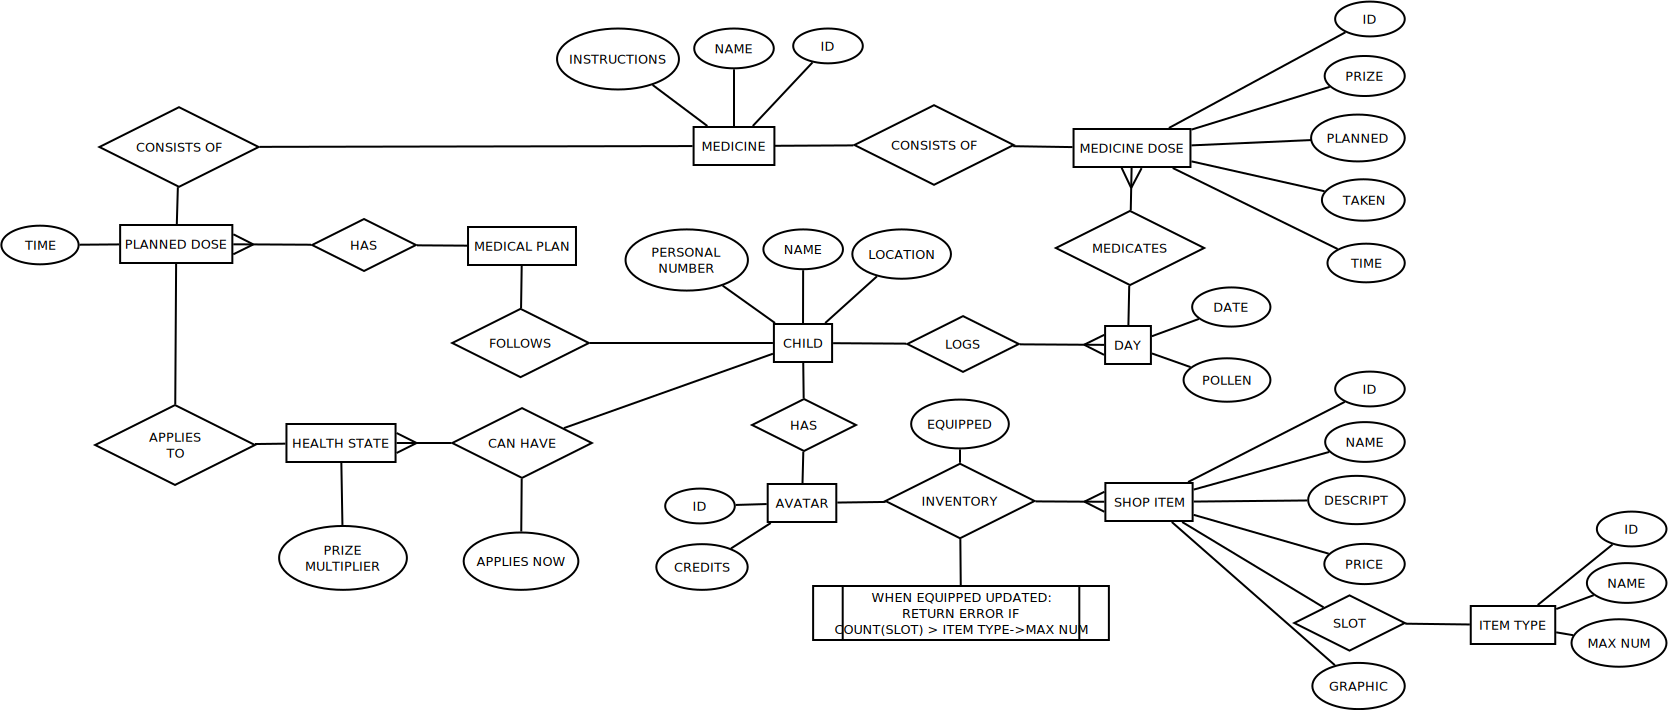
\includegraphics[width=0.9\paperheight]{Pictures/ArchPictures/BLOPP_DB_ER_diagram.png}
	\caption{ER diagram for the BLOPP database}
	\label{fig:db-er-diagram}
\end{figure}
\end{landscape}
%\subsection{Database \LaTeX{} export for database}
% phpMyAdmin LaTeX Dump
% version 2.5.6
% http://www.phpmyadmin.net
%
% Host: mysql.stud.ntnu.no
% Generation Time: Sep 12, 2012 at 09:14 AM
% Server version: 5.0.96
% PHP Version: 5.2.4-2ubuntu5.25
% 
% Database : `yngvesva_blopp`
% 

%
% Structure: AVATARS
%
 \begin{longtable}{|l|c|c|c|} 
 \caption{Structure of table AVATARS} \label{tab:AVATARS-structure} \\
 \hline \multicolumn{1}{|c|}{\textbf{Field}} & \multicolumn{1}{|c|}{\textbf{Type}} & \multicolumn{1}{|c|}{\textbf{Null}} & \multicolumn{1}{|c|}{\textbf{Default}} \\ \hline \hline
\endfirsthead
 \caption{Structure of table AVATARS (continued)} \\ 
 \hline \multicolumn{1}{|c|}{\textbf{Field}} & \multicolumn{1}{|c|}{\textbf{Type}} & \multicolumn{1}{|c|}{\textbf{Null}} & \multicolumn{1}{|c|}{\textbf{Default}} \\ \hline \hline \endhead \endfoot \textbf{\textit{id}} & int(11) & Yes & NULL \\ \hline 
credits & int(11) & Yes & 0 \\ \hline 
\textbf{inventory\_id} & int(11) & Yes & NULL \\ \hline 
 \end{longtable}

%
% Structure: AVATAR_INVENTORIES
%
 \begin{longtable}{|l|c|c|c|} 
 \caption{Structure of table AVATAR\_INVENTORIES} \label{tab:AVATAR_INVENTORIES-structure} \\
 \hline \multicolumn{1}{|c|}{\textbf{Field}} & \multicolumn{1}{|c|}{\textbf{Type}} & \multicolumn{1}{|c|}{\textbf{Null}} & \multicolumn{1}{|c|}{\textbf{Default}} \\ \hline \hline
\endfirsthead
 \caption{Structure of table AVATAR\_INVENTORIES (continued)} \\ 
 \hline \multicolumn{1}{|c|}{\textbf{Field}} & \multicolumn{1}{|c|}{\textbf{Type}} & \multicolumn{1}{|c|}{\textbf{Null}} & \multicolumn{1}{|c|}{\textbf{Default}} \\ \hline \hline \endhead \endfoot \textbf{\textit{id}} & int(11) & Yes & 0 \\ \hline 
\textbf{shop\_item\_id} & int(11) & Yes & NULL \\ \hline 
equipped & int(1) & Yes & 0 \\ \hline 
avatar\_id & int(11) & Yes & NULL \\ \hline 
 \end{longtable}

%
% Structure: AVATAR_ITEM_SLOTS
%
 \begin{longtable}{|l|c|c|c|} 
 \caption{Structure of table AVATAR\_ITEM\_SLOTS} \label{tab:AVATAR_ITEM_SLOTS-structure} \\
 \hline \multicolumn{1}{|c|}{\textbf{Field}} & \multicolumn{1}{|c|}{\textbf{Type}} & \multicolumn{1}{|c|}{\textbf{Null}} & \multicolumn{1}{|c|}{\textbf{Default}} \\ \hline \hline
\endfirsthead
 \caption{Structure of table AVATAR\_ITEM\_SLOTS (continued)} \\ 
 \hline \multicolumn{1}{|c|}{\textbf{Field}} & \multicolumn{1}{|c|}{\textbf{Type}} & \multicolumn{1}{|c|}{\textbf{Null}} & \multicolumn{1}{|c|}{\textbf{Default}} \\ \hline \hline \endhead \endfoot \textbf{\textit{id}} & int(11) & Yes & NULL \\ \hline 
name & varchar(128) & Yes & NULL \\ \hline 
equip\_limit & int(4) & Yes & NULL \\ \hline 
x & double & Yes & NULL \\ \hline 
y & double & Yes & NULL \\ \hline 
 \end{longtable}

%
% Structure: CHILDREN
%
 \begin{longtable}{|l|c|c|c|} 
 \caption{Structure of table CHILDREN} \label{tab:CHILDREN-structure} \\
 \hline \multicolumn{1}{|c|}{\textbf{Field}} & \multicolumn{1}{|c|}{\textbf{Type}} & \multicolumn{1}{|c|}{\textbf{Null}} & \multicolumn{1}{|c|}{\textbf{Default}} \\ \hline \hline
\endfirsthead
 \caption{Structure of table CHILDREN (continued)} \\ 
 \hline \multicolumn{1}{|c|}{\textbf{Field}} & \multicolumn{1}{|c|}{\textbf{Type}} & \multicolumn{1}{|c|}{\textbf{Null}} & \multicolumn{1}{|c|}{\textbf{Default}} \\ \hline \hline \endhead \endfoot \textbf{\textit{id}} & int(11) & Yes & NULL \\ \hline 
name & varchar(100) & Yes & NULL \\ \hline 
\textbf{pers\_num} & int(11) & Yes & NULL \\ \hline 
\textbf{medical\_plan\_id} & int(11) & Yes & NULL \\ \hline 
\textbf{avatar\_id} & int(11) & Yes & NULL \\ \hline 
\textbf{child\_health\_state\_id} & int(11) & Yes & NULL \\ \hline 
 \end{longtable}

%
% Structure: CHILDREN_LOG_DAYS
%
 \begin{longtable}{|l|c|c|c|} 
 \caption{Structure of table CHILDREN\_LOG\_DAYS} \label{tab:CHILDREN_LOG_DAYS-structure} \\
 \hline \multicolumn{1}{|c|}{\textbf{Field}} & \multicolumn{1}{|c|}{\textbf{Type}} & \multicolumn{1}{|c|}{\textbf{Null}} & \multicolumn{1}{|c|}{\textbf{Default}} \\ \hline \hline
\endfirsthead
 \caption{Structure of table CHILDREN\_LOG\_DAYS (continued)} \\ 
 \hline \multicolumn{1}{|c|}{\textbf{Field}} & \multicolumn{1}{|c|}{\textbf{Type}} & \multicolumn{1}{|c|}{\textbf{Null}} & \multicolumn{1}{|c|}{\textbf{Default}} \\ \hline \hline \endhead \endfoot \textbf{\textit{date}} & date & Yes & NULL \\ \hline 
\textbf{\textit{child\_id}} & int(11) & Yes & 0 \\ \hline 
pollen\_state\_id & int(11) & Yes & NULL \\ \hline 
 \end{longtable}

%
% Structure: CHILD_HEALTH_STATES
%
 \begin{longtable}{|l|c|c|c|} 
 \caption{Structure of table CHILD\_HEALTH\_STATES} \label{tab:CHILD_HEALTH_STATES-structure} \\
 \hline \multicolumn{1}{|c|}{\textbf{Field}} & \multicolumn{1}{|c|}{\textbf{Type}} & \multicolumn{1}{|c|}{\textbf{Null}} & \multicolumn{1}{|c|}{\textbf{Default}} \\ \hline \hline
\endfirsthead
 \caption{Structure of table CHILD\_HEALTH\_STATES (continued)} \\ 
 \hline \multicolumn{1}{|c|}{\textbf{Field}} & \multicolumn{1}{|c|}{\textbf{Type}} & \multicolumn{1}{|c|}{\textbf{Null}} & \multicolumn{1}{|c|}{\textbf{Default}} \\ \hline \hline \endhead \endfoot \textbf{\textit{id}} & int(11) & Yes & NULL \\ \hline 
health\_state\_id & int(11) & Yes & NULL \\ \hline 
applies\_now & int(1) & Yes & NULL \\ \hline 
 \end{longtable}

%
% Structure: DAY_MEDICINE_DOSES
%
 \begin{longtable}{|l|c|c|c|} 
 \caption{Structure of table DAY\_MEDICINE\_DOSES} \label{tab:DAY_MEDICINE_DOSES-structure} \\
 \hline \multicolumn{1}{|c|}{\textbf{Field}} & \multicolumn{1}{|c|}{\textbf{Type}} & \multicolumn{1}{|c|}{\textbf{Null}} & \multicolumn{1}{|c|}{\textbf{Default}} \\ \hline \hline
\endfirsthead
 \caption{Structure of table DAY\_MEDICINE\_DOSES (continued)} \\ 
 \hline \multicolumn{1}{|c|}{\textbf{Field}} & \multicolumn{1}{|c|}{\textbf{Type}} & \multicolumn{1}{|c|}{\textbf{Null}} & \multicolumn{1}{|c|}{\textbf{Default}} \\ \hline \hline \endhead \endfoot \textbf{\textit{id}} & int(11) & Yes & NULL \\ \hline 
prize & int(8) & Yes & NULL \\ \hline 
planned & int(1) & Yes & NULL \\ \hline 
taken & int(1) & Yes & NULL \\ \hline 
time & datetime & Yes & NULL \\ \hline 
day\_date & date & Yes & NULL \\ \hline 
child\_id & int(11) & Yes & NULL \\ \hline 
medicine\_id & int(11) & Yes & NULL \\ \hline 
 \end{longtable}

%
% Structure: HEALTH_STATES
%
 \begin{longtable}{|l|c|c|c|} 
 \caption{Structure of table HEALTH\_STATES} \label{tab:HEALTH_STATES-structure} \\
 \hline \multicolumn{1}{|c|}{\textbf{Field}} & \multicolumn{1}{|c|}{\textbf{Type}} & \multicolumn{1}{|c|}{\textbf{Null}} & \multicolumn{1}{|c|}{\textbf{Default}} \\ \hline \hline
\endfirsthead
 \caption{Structure of table HEALTH\_STATES (continued)} \\ 
 \hline \multicolumn{1}{|c|}{\textbf{Field}} & \multicolumn{1}{|c|}{\textbf{Type}} & \multicolumn{1}{|c|}{\textbf{Null}} & \multicolumn{1}{|c|}{\textbf{Default}} \\ \hline \hline \endhead \endfoot \textbf{\textit{id}} & int(11) & Yes & NULL \\ \hline 
label & varchar(256) & Yes & NULL \\ \hline 
 \end{longtable}

%
% Structure: MEDICAL_PLANS
%
 \begin{longtable}{|l|c|c|c|} 
 \caption{Structure of table MEDICAL\_PLANS} \label{tab:MEDICAL_PLANS-structure} \\
 \hline \multicolumn{1}{|c|}{\textbf{Field}} & \multicolumn{1}{|c|}{\textbf{Type}} & \multicolumn{1}{|c|}{\textbf{Null}} & \multicolumn{1}{|c|}{\textbf{Default}} \\ \hline \hline
\endfirsthead
 \caption{Structure of table MEDICAL\_PLANS (continued)} \\ 
 \hline \multicolumn{1}{|c|}{\textbf{Field}} & \multicolumn{1}{|c|}{\textbf{Type}} & \multicolumn{1}{|c|}{\textbf{Null}} & \multicolumn{1}{|c|}{\textbf{Default}} \\ \hline \hline \endhead \endfoot \textbf{\textit{id}} & int(11) & Yes & NULL \\ \hline 
label & varchar(256) & Yes & NULL \\ \hline 
 \end{longtable}

%
% Structure: MEDICAL_PLAN_DOSES
%
 \begin{longtable}{|l|c|c|c|} 
 \caption{Structure of table MEDICAL\_PLAN\_DOSES} \label{tab:MEDICAL_PLAN_DOSES-structure} \\
 \hline \multicolumn{1}{|c|}{\textbf{Field}} & \multicolumn{1}{|c|}{\textbf{Type}} & \multicolumn{1}{|c|}{\textbf{Null}} & \multicolumn{1}{|c|}{\textbf{Default}} \\ \hline \hline
\endfirsthead
 \caption{Structure of table MEDICAL\_PLAN\_DOSES (continued)} \\ 
 \hline \multicolumn{1}{|c|}{\textbf{Field}} & \multicolumn{1}{|c|}{\textbf{Type}} & \multicolumn{1}{|c|}{\textbf{Null}} & \multicolumn{1}{|c|}{\textbf{Default}} \\ \hline \hline \endhead \endfoot \textbf{\textit{id}} & int(11) & Yes & NULL \\ \hline 
medical\_plan\_id & int(11) & Yes & NULL \\ \hline 
health\_state\_id & int(11) & Yes & NULL \\ \hline 
time & time & Yes & NULL \\ \hline 
medicine\_id & int(11) & Yes & NULL \\ \hline 
 \end{longtable}

%
% Structure: MEDICINES
%
 \begin{longtable}{|l|c|c|c|} 
 \caption{Structure of table MEDICINES} \label{tab:MEDICINES-structure} \\
 \hline \multicolumn{1}{|c|}{\textbf{Field}} & \multicolumn{1}{|c|}{\textbf{Type}} & \multicolumn{1}{|c|}{\textbf{Null}} & \multicolumn{1}{|c|}{\textbf{Default}} \\ \hline \hline
\endfirsthead
 \caption{Structure of table MEDICINES (continued)} \\ 
 \hline \multicolumn{1}{|c|}{\textbf{Field}} & \multicolumn{1}{|c|}{\textbf{Type}} & \multicolumn{1}{|c|}{\textbf{Null}} & \multicolumn{1}{|c|}{\textbf{Default}} \\ \hline \hline \endhead \endfoot \textbf{\textit{id}} & int(11) & Yes & NULL \\ \hline 
name & varchar(256) & Yes & NULL \\ \hline 
instructions\_id & int(11) & Yes & NULL \\ \hline 
 \end{longtable}

%
% Structure: POLLEN_STATES
%
 \begin{longtable}{|l|c|c|c|} 
 \caption{Structure of table POLLEN\_STATES} \label{tab:POLLEN_STATES-structure} \\
 \hline \multicolumn{1}{|c|}{\textbf{Field}} & \multicolumn{1}{|c|}{\textbf{Type}} & \multicolumn{1}{|c|}{\textbf{Null}} & \multicolumn{1}{|c|}{\textbf{Default}} \\ \hline \hline
\endfirsthead
 \caption{Structure of table POLLEN\_STATES (continued)} \\ 
 \hline \multicolumn{1}{|c|}{\textbf{Field}} & \multicolumn{1}{|c|}{\textbf{Type}} & \multicolumn{1}{|c|}{\textbf{Null}} & \multicolumn{1}{|c|}{\textbf{Default}} \\ \hline \hline \endhead \endfoot \textbf{\textit{id}} & int(11) & Yes & NULL \\ \hline 
label & varchar(256) & Yes & NULL \\ \hline 
 \end{longtable}

%
% Structure: SHOP_ITEMS
%
 \begin{longtable}{|l|c|c|c|} 
 \caption{Structure of table SHOP\_ITEMS} \label{tab:SHOP_ITEMS-structure} \\
 \hline \multicolumn{1}{|c|}{\textbf{Field}} & \multicolumn{1}{|c|}{\textbf{Type}} & \multicolumn{1}{|c|}{\textbf{Null}} & \multicolumn{1}{|c|}{\textbf{Default}} \\ \hline \hline
\endfirsthead
 \caption{Structure of table SHOP\_ITEMS (continued)} \\ 
 \hline \multicolumn{1}{|c|}{\textbf{Field}} & \multicolumn{1}{|c|}{\textbf{Type}} & \multicolumn{1}{|c|}{\textbf{Null}} & \multicolumn{1}{|c|}{\textbf{Default}} \\ \hline \hline \endhead \endfoot \textbf{\textit{id}} & int(11) & Yes & NULL \\ \hline 
price & int(11) & Yes & 0 \\ \hline 
slot\_id & int(11) & Yes & NULL \\ \hline 
graphic & mediumblob & Yes & NULL \\ \hline 
name & varchar(64) & Yes & NULL \\ \hline 
description & varchar(256) & Yes & NULL \\ \hline 
 \end{longtable}
\subsection{Databse Implementation}
\label{sec:databaseImplementaion}
The final implemented databse architecture is displayed in figure \ref{fig:databaseImplementation}. The tables related to
the avatar: \code{AVATAR}, \code{AVATAR\_INVENTORIES}, \code{SHOP\_ITEMS} and \code{AVATAR\_ITEM\_SLOTS} are not used in the system because 
the avatar idea was put on hold. The rows \code{location\_latitude} and \code{location\_longtitude} in the table \code{CHILDREN} are also
not used because we did not implement updating the pollen feed based on current location.

The arrows symbolize relations, where the big end is the refereced key and the small end is the foreign key.

\begin{figure}
	\begin{center}
	\begin{sideways}
		\includegraphics[width=0.8\paperheight]{Pictures/ArchPictures/DatabaseImplementation}
	\end{sideways}
	\end{center}
	\caption{Implemented Database Architecture}
	\label{fig:databaseImplementation}
\end{figure}
\subsection{Database Access Layer}
\label{sec:databaseAccessLayer}
The database access layer consists of 14 PHP files hosted at			%TODO: update this number ? 
\url{http://folk.ntnu.no/yngvesva/blopp/}:
\begin{description}
    \item[add\_child.php] Takes a name, personal number (SSN) and a list of states (integer IDs) that the child can have. 
    	Creates an entry in the \code{CHILDREN} table for the child, and a medical plan entry. Also creates an entry 
    	in \code{CHILD\_HEALTH\_STATES} for all the states the child can have. Returns the generated \code{medical\_plan\_id}.
    \item[add\_plan\_dose.php] Inserts a new entry in the \code{MEDICAL\_PLAN\_DOSES} table for the given child, with the parameters 'health state', 'dose of the given medicine' and a timestamp. This is the primary module used to alter medical plans. Returns the ID of the
  		added dose.
    \item[dose\_is\_taken.php] Check if a dose of a planned medicine has been taken that day. Takes an \code{id} of an entry in
    	the table \code{MEDICAL\_PLAN\_DOSES} as input.
    \item[get\_available\_child\_states.php] Takes a \code{child\_id} and returns a list of the labels (colors, names) and IDs of the 
    	states the child can have.
    \item[get\_child.php] Takes an ID of a child and returns all the columns for the given ID in the \code{CHILDREN} table.
    \item[get\_child\_state.php] Accepts a child ID and returns the ID and label of the current state of the child.
    \item[get\_doses\_for\_current\_state.php] Takes a child ID and returns a list of planned doses of medicines that are not 
    	taken that day. The fields of each entry are: \code{id}, \code{medical\_plan\_id}, \code{health\_state\_id}, \code{time}, 
    	\code{medicine\_id}, \code{medicine\_karotz\_color} and \code{medicine\_name}.
    \item[get\_instructions.php] Get instructions (image, effect description and usage description) for a given medicine by ID.
    \item[get\_log\_days\_for\_child.php] For the calendar in GAPP, it was advantageous to have a database access method that
  		could return a list of days in a month with the child health state for each day, and a list of doses taken on that day. 
  		\code{get\_log\_days\_for\_child.php} accomplishes this by using the table \code{CHILDREN\_LOG\_DAYS} to find the latest recorded
  		health state before the given month started. Then it iterates through all the days, checking if there are any days in the month
  		where the status changes, and adding all doses, taken from \code{DAY\_MEDICINE\_DOSES}, on that day. The method takes a \code{child id},
  		and two optional parameters \code{month} and \code{year}. If the month and year are not set, the values for the current days
  		are used.
    \item[get\_log\_for\_child.php] Returns all registered entries in the table \code{DAY\_MEDICINE\_DOSES} for the day for a given child (id) 
    	during the given month during the given year.
    \item[register\_medicine\_taken.php] Register a dose of medicine taken. Accepts a post object with the fields \code{child\_id}, \code{medicine\_id}, 
    	\code{time}, \code{day\_date}, \code{health\_state\_id} and \code{medical\_plan\_dose\_id}. If there is an entry for that dose id that day, the method does 
    	nothing and simply returns $unique=false$. Otherwise, it calculates a reward, and updates \code{DAY\_MEDICINE\_DOSES} with the entry. 
    	Returns the reward for that dose. Then it adds the calculated reward to the child's total credits in the \code{CHILDREN} table. If 
  		no time is given, a default time of 00:00:01 is set.
    \item[remove\_plan\_dose.php] Deletes the entry in the table \code{MEDICAL\_PLAN\_DOSES} which corresponds to a given id. Returns
  		the number of deleted rows.
    \item[remove\_plan\_medicine\_at\_time.php] During development of GAPP, it was discovered that using a
  		combination of \code{child\_id}, \code{medicine\_id} and \code{time} as the key for removing elements in the \code{MEDICAL\_PLAN\_DOSES}
  		table would be easier than using an ID. Therefore the need for this module arised, and it simply removes all entries in the
  		table that fit the criteria.
    \item[set\_child\_state.php] Takes a child ID and a state ID and sets the current state of the given child to the specific state given as input. Also updates 
    	the table \code{CHILDREN\_LOG\_DAYS} with the given health state.
\end{description}
%\include{DocumentTemplates/DocumentTemplates}
\chapter{Overall Test Plan}
\label{chap:testPlan}
The following chapter concerns the overall testplan for the project, and it contains general
information about testing and what tests we aimed to perform. The template for our 
tests can be found in table \ref{tab:testtable}, while the tests that were performed can be found
in table \ref{tab:listoftests}.
\\
%\section{Introduction} Almost the same as the section above, so I merge them
We test the system to 
make sure that our applications are easy to use, and works the way they're intended,
ensuring that the delivered product fulfills the requirement specifications. We 
will document the most important tests with a description of the test we performed, what we 
discovered during the test, and what we did to fix eventual problems that surfaced 
during the test.
%Needs references
%rly?

\section{Test methods}
There are different test methods that can be used. The outer points are black-box and 
white-box testing, but we can also do gray-box testing, a combination of the two.

\subsection{Black-box testing}
This method tests the functionality of the system. Black-box testing means we feed 
something in and then see if the result we get out is the same as the one we were 
expecting. This means that knowledge about the code and structure of the system 
we are testing is unknown and irrelevant to the test. The tests will then be based on 
external software descriptions like the functional requirements for the system.

\subsection{White-box testing}
This method of testing concerns itself with testing the internal structures of a 
system. This means knowledge about structure and code is required to run the test, 
and we require knowledge about the programming to design the test cases. Normally 
this type of testing is performed at unit level, but can also be used on the system 
as a whole. The problems detected by white box testing is technical, and it can not 
detect whether or not a program is fulfilling it's functional requirements.

\section{Test levels}
There are different types and levels of testing. Usability testing focuses on the 
general, graphical and functional part of the system, how easy the applications is 
to use for the typical end users. There are low level tests testing the smaller parts 
of the system, typically classes or methods, and there are high level tests, that 
tests the system, or parts of the system.

\subsection{Unit testing}
The lowest form of testing is unit testing. This is intended to test the smallest 
units of the system, namely the methods, classes and variables, making sure that each 
of these parts works as expected. 

\subsection{Module testing}
Once the smaller parts of the system has been tested, we also test the coordination 
between these parts, by testing that the entire module works as we intended.

\subsection{Integration and System testing}
When all of the individually tested modules works as intended, we test 
that the different parts of the system works together, taking 
small to medium parts of the system into the test, while the system tests will test the 
system as a whole. That means that these tests test communication between
the different modules and interfaces.

\section{Testing approach}	
We decided to use both black box and white box testing for our system. We did 
two bigger usability tests, where we applied black box testing on both. We would have preferred to
do some more usability testing, however, since we had to implement the system from scratch, we decided
to start with one paper prototype usability test to get initial thoughts from the potential users. Then 
we moved on with implementing the system before we again did a bigger usability test, this 
time  with children. We used the implemented applications and the distraction sequence with the Karotz.
This meant we had to do alot of unit and integration testing on the system during the implementation. 

All of our tests will follow the template presented in table \ref{tab:testtable}.
\begin{table}
	\begin{center}
		\begin{tabular}{|p{4.0cm}|p{8.0cm}|}
			\hline
			\bf{Item} & \bf{Description}\\
			\hline
			\bf{ID} & Identifier for the test\\
			\bf{Description} & Description of the test\\
			\bf{Date} & Date of the test\\
			\bf{Responsible} & The person responsible for the test\\
			\bf{Subject} & The subject being tested (typically a unit or part of the system)\\
			\bf{Precondition} & The conditions we assume to be in place when the test is started\\
			\bf{Steps} & The steps to perform\\
			\hline
			\bf{Results} & Results after the test was performed\\
			\hline
		\end{tabular}
	\end{center}
	\caption{Test template}
	\label{tab:testtable}
\end{table}

The tests done during this project is listed in table \ref{tab:listoftests}, with the testID, brief description of the test
and during what part of the project it was done.
\begin{table}
	\begin{center}
		\begin{tabular}{|p{3.3cm}|p{10.0cm}|p{4.0cm}|}
			%\endfirsthead
			%\endhead
			%\endfoot
			%\caption{List of tests}
			%\endlastfoot
			\hline
				\bf{ID} & \bf{Description}& \bf{Time of test}\\
			\hline
				USABILITY0.1 &	 Paper prototype test &  						04.09.12 (section \ref{sec:paperprototypetest})\\
				\hline
				USABILITY02 & 	Usability testing of the system on children & 			30.10.12 (table \ref{tab:usability5.1})\\
				\hline
				UNIT1.1 &		Test of GUI for GAPP & 												17.09.12 (table \ref{tab:unit1.1})\\
				\hline
				UNIT1.2 & 		Test of GUI for CAPP & 												17.09.12 (table \ref{tab:unit1.2})\\
				\hline
				UNIT2.1 & 		Test of the CAPP distraction sequence & 									30.09.12 (table \ref{tab:unit2.1})\\
				\hline
				UNIT2.2 & 		Test of the database connection & 										26.09.12 (table \ref{tab:unit2.2})\\
				\hline
				UNIT2.3 & 		Testing of SQL-queries &		 										30.09.12 (table \ref{tab:unit2.3})\\
				\hline
				UNIT3.1 & 		Test that alarm is given independently of phone state & 							14.10.12 (table \ref{tab:unit3.1})\\
				\hline
				UNIT3.2 & 		Test that the correct days is colored in the log &								09.10.12 (table \ref{tab:unit3.2})\\
				\hline
				UNIT3.3 & 		Test that the karotz notification is given at the correct time & 						09.10.12 (table \ref{tab:unit3.3})\\
				\hline
				UNIT3.4 & 		Test that the karotz distraction runs after recieving the notification and starting the sequence & 	09.10.12 (table \ref{tab:unit3.4})\\
				\hline
				UNIT3.5 & 		Test that the notifications with multiple doses makes the correct amount of medications & 		11.10.12 (table \ref{tab:unit3.5})\\
				\hline
				UNIT4.1 & 		Test that the right instructions are downloaded and shown on the instructions menu screen & 	18.10.12 (table \ref{tab:unit4.1})\\
				\hline
				UNIT5.1 & 		Test of the web access module \code{add\_child.php} & 							30.10.12 (table \ref{tab:unit5.1})\\
				\hline
				UNIT5.2 & 		Test of the web access module \code{add\_plan\_dose.php} & 						01.11.12 (table \ref{tab:unit5.2})\\
				\hline
				UNIT5.3 & 		Test of the web access module \code{dose\_is\_taken.php}. & 						01.11.12 (table \ref{tab:unit5.3})\\
				\hline
				UNIT5.4 & 		Test of the web access module \code{get\_available\_child\_states.php}. & 				01.11.12 (table \ref{tab:unit5.4})\\
				\hline
				UNIT5.5 & 		Test of the web access module \code{get\_child.php}. & 							01.11.12 (table \ref{tab:unit5.5})\\
				\hline
				UNIT5.6 & 		Test of the web access module \code{get\_child\_state.php}. & 						01.11.12 (table \ref{tab:unit5.6})\\
				\hline
				UNIT5.7 & 		Test of the web access module \code{get\_doses\_for\_current\_state.php}. & 			01.11.12 (table \ref{tab:unit5.7})\\
				\hline
				UNIT5.8 & 		Test of the web access module \code{get\_instructions.php}. & 						01.11.12 (table \ref{tab:unit5.8})\\
				\hline
				UNIT5.9 & 		Test of the web access module \code{get\_log\_days\_for\_child.php}. & 				03.11.12 (table \ref{tab:unit5.9})\\
				\hline
				UNIT5.10 & 		Test of the web access module \code{get\_log\_for\_child.php}. & 					03.11.12 (table \ref{tab:unit5.10})\\
				\hline
				UNIT5.11 & 		Test of the web access module \code{get\_plan.php}. & 							04.11.12 (table \ref{tab:unit5.11})\\
				\hline
				UNIT5.12 & 		Test of the web access module \code{register\_medicine\_taken.php}. & 				04.11.12 (table \ref{tab:unit5.12})\\
				\hline
				UNIT5.13 & 		Test of the web access module \code{remove\_plan\_dose.php}. & 					04.11.12 (table \ref{tab:unit5.13})\\
				\hline
				UNIT5.14 & 		Test of the web access module \code{remove\_plan\_medicine\_at\_time.php}. & 			04.11.12 (table \ref{tab:unit5.14})\\
				\hline
				UNIT5.15 & 		Test of the web access module \code{set\_child\_state.php}. & 						05.11.12 (table \ref{tab:unit5.15})\\
				\hline
				INTEGRATION5.1 & Test of CAPPs alarm and distraction sequences. & 							06.11.12 (table \ref{tab:integration5.1})\\
				\hline
				INTEGRATION5.2 & Testing that the log updates correctly based on registered medication and pollen feed. & 	06.11.12 (table \ref{tab:integration5.2})\\
				\hline
				INTEGRATION5.3 & Testing that the medicationplans is correctly registered to their respective healthstates. & 	05.11.12 (table \ref{tab:integration5.3})\\
			\hline
		\end{tabular}
	\end{center}
	\caption{List of tests}
	\label{tab:listoftests}
\end{table}
\blankpage{}
\subsection{Sprints}
\label{sec:sprints}
This section gives a short description of how the Scrum development method was used in the project. 
For a general explanation of Scrum see Section \ref{sec:scrum}.

\subsubsection{Sprint duration}
We decided on having 14 day sprints. After discussions with the customer,
we agreed that this would be a suitable duration, due to the fact 
that the documentation needed for each sprint would be time consuming 
for shorter sprints.

\subsubsection{Sprint Planning Meeting}
To start each sprint, we held a sprint planning meeting. During this meeting, we discussed which user 
stories/epics from the sprint backlog should be worked on during the sprint. The reason behind such a 
meeting is to make sure the team is on updated on the goals for the following sprint. To decide what 
user stories/epics should be chosen, the priorities given by the customer was used as a pinpoint. If 
the customer wanted to make any changes during a sprint, the changes were noted and discussed during 
the next sprint planning meeting.

\subsubsection{Daily Standup}
The daily standups (also commonly known as daily scrum meeting) were held on Mondays, Wednesdays and 
Fridays. The team decided on this semi-daily recurrence since not all team members were able to work 
on the project every day. During the standup meetings all team members would answer three questions: 
what have you done since our last meeting, what will you work on until the next meeting, and what 
problems did occur since our last meeting?

Answering these questions gave a certain status update, and made it easier to re-assign team members 
to tasks if needed. During the standups all technical discussions were discouraged. If any technical 
questions arose, the people involved would discuss this after the meeting, to make sure they were not 
wasting other people's time. Each standup had a max allowed length of 15 minutes. 

\subsubsection{Sprint retrospective}
The sprint retrospective is the written conclusion of the sprint. A meeting was held at the end of each 
sprint, discussing the results throughout the sprint, both finished and unfinished tasks. The tasks not 
completed were moved to the next sprint, and the reason for the task not being completed was stated in 
the sprint report. 

The sprint report also includes an update of the sprint backlog, along with an overview of how much time 
was spent on each task, making it easy to compare to the time estimate. 

The sprint retrospective also contains a burndown chart, giving a visual representation of how the team 
worked during the sprint.

For each sprint we answered the following questions: 
\begin{itemize}
	\item What went well?
	\item What shall we start doing?
	\item What could have gone better?
	\item What should we stop doing?
\end{itemize}
%TODO: the questions

\subsubsection{Explanation of Sprint Backlog}
The sprint backlog is a task management tool to document and ensure the progress of the sprint. Each task the 
team chooses to focus on in the sprint is enlisted. The task is given an ID and already has a name. The 
Function number is an hour-independent number telling how difficult the team expects the task to be. The 
base number represents how many hours the team expects to work to finish one story point. The base number multiplied 
with the function number for a task gives the estimated work hours needed to finish a task.

The base number may change from sprint to sprint, but not during a sprint. The team did an evaluation of 
the base number in advance of each sprint, to make good estimates.

The name column is used to keep track of who is responsible for the task. This may change during the sprint, 
but the sprint backlog should always be showing the correct info.

Based on how many team members are available and how many work hours they may put in, the team gives an 
expected decrease of the story points left. This is reflected in the sprint burndown chart for each sprint, 
as a straight decreasing line.
\chapter{Usability Testing}
\label{sec:Usabilitytesting}
This section will explain what usability testing is, and what we did during our project relating to usability testing.

\section{What is usability testing}
Usability testing is a way to test your system on users, using the interaction design of the system. Usually this entails setting up 
a few tasks for a user, giving the user access to the system and seeing how well the user is able to solve the tasks given in the test
with the system provided. The usability testing focuses on the main functionality rather than on the details. 

\section{How to do usability testing}
The test usually starts with the tester explaining for the user the different parts of the systems being used, and that it's the system being
tested, not the user. The tester also explains that this means the user can't do anything wrong, if there is something the user doesn't 
understand, that is fine. The tester observe what the user finds hard, or can't do at all, and notes this down as things that might have
to be changed on the system. 

At last, the user is given an evaluation form of the system, typically a SUS-form (System Usability Scale), and time to talk about
how well they felt the system helped them solve the tasks given. %Add reference to SUS?

\section{Usability testing in our project}
Our project largely implements user interraction, and usability testing plays a key role in getting a good result, since so much
of the project is centered around the user interface. We started the project with an early paper prototype test, to get some feedback on the ideas
we got after the workshop we did with the interaction design group. After this we worked for some time on implementing the system, before we late in
the project did a full usability test using the hallway method, testing our system on children to see if it helped them take their medicine, and seeing
if there was some bugs or things we could implement better.

\subsection{Paper prototype test}
\label{sec:paperprototypetest}
In the early stages of development, it might be useful to do a paper prototype test. This test is done by making a prototype of the user interface on paper, 
and having one person (the "computer") change between the different paper screens based on what the user being tested clicks on. 

We did some early paper prototype testing in our project, on the 4th of September. After our workshop we had made some screen layout mockups, see figure \ref{fig:paperprototype}, 
and we wanted to test how user friendly these were.

\begin{figure}
	%\vspace{-4cm}
	%\hspace{4cm}
	\center
		\includegraphics[width=0.8\paperheight, angle=90]{Pictures/PaperprototypeScaled}

	\caption[Paper prototype]{The screens of the paper prototype: a) The GAPP mainscreen. 

								b) GAPP new medication screen.
								c) GAPP settings screen
								d) GAPP log screen.
								e) Notification on phone
								f) One of the CAPP distraction screens.
								g) The CAPP reward screen
								h) CAPP shop screen
								i) CAPP avatar screen, after buying skateboard in the shop
								j) the GAPP manual screen}
	\label{fig:paperprototype}
\end{figure}

The test was done with the expert review method. We had a person from NAAF come for the test, to solve the tasks with the system we provided. We chose to do the expert
review mainly because our funder was interested in seeing how the project was proceeding. NAAF is also the main provider of information such as instructions and 
how the medical plans looks, so having one of them see the system was helpful, as we at this point was uncertain about alot of these things.

From the development group, Eirik and Aleks attended the test. Eirik played the part of the computer, while Aleks introduced the test, explained the system and handled
any other talking that needed to be done.\\
The preconditions we assumed to be present for the CAPP was:
\begin{itemize}
	\item A paper prototype with the correct screens.
	\item Basic knowledge of Android devices in the user being tested.
	\item An active notification for taking medicine on the android device.
\end{itemize}
for GAPP these precondition were:
\begin{itemize}
	\item A paper prototype with the correct screens.
	\item Basic knowledge of android devices in the user being tested.
	\item The correct medication plans and medicines registered in the system.
\end{itemize}

We had prepared a set of tasks for each of our two android applications, CAPP and GAPP. We did not have a functional application for the karotz at this point, and it was difficult to
test this with a paper prototype, so we chose to leave that part out of this test. The cases can be seen in table \ref{tab:capptasks} and table \ref{tab:gapptasks}.

\begin{table}[h]
	\begin{center}
		\begin{tabular}{|p{1.0cm}|p{10.0cm}|}
			\hline
			\bf{Task} & \bf{Description}\\
			\hline
			\bf{1} & There is an active notification for medication on the phone, follow the instructions given by the android device.\\
			\bf{2} & Go to the shop in CAPP and buy a skateboard for the avatar.\\
			\hline
		\end{tabular}
	\end{center}
	\caption{The tasks for CAPP}
	\label{tab:capptasks}
\end{table}

\begin{table}[h]
	\begin{center}
		\begin{tabular}{|p{1.0cm}|p{10.0cm}|}
			\hline
			\bf{Task} & \bf{Description}\\
			\hline
			\bf{1} & Open GAPP.\\
			\bf{2} & Register use of "Medisin 1" on 4th of september.\\
			\bf{3} & Check for more iformation on correct usage of "Medisin 2".\\
			\hline
		\end{tabular}
	\end{center}
	\caption{The tasks for GAPP}
	\label{tab:gapptasks}
\end{table}

This test gave us some strong feedback on what parts of the system worked well, and what didn't make sense at all. We also sat down and had an interview with
the test person after the test regarding the best way to present the information we would get from NAAF.
Some of the problems the test person had might be credited to her being inexperienced with android devices, but we noted down these problems aswell.
 In short the paper prototype test gave us the following results:

\begin{itemize}
	\item Having the reminder as a notification is insufficient. The test person had trouble noticing it even though she was told it would be there.
	\item CAPP have to inform how many times you should press the medicine during medication.
	\item The rewardscreen in CAPP is not intuitive enough.
	\item The main menu in GAPP needs a complete rework, the menu system was not easy to understand.
	\item The Log have to be clearer on how to register medicines, and which medicines is already registered.
	\item There is no back button in the application. This is a problem with android experience, and we didn't implement a back button in the end.
	\item The Information about correct use of medicines was not easily accessible.
\end{itemize} 
The paper prototype led to a major overhaul of the user interface.

\subsection{Usability testing of the distraction}
\label{sec:usabilitytestonchildren}
Since our system is targeted towards children it was important to test the system properly on children, to see if the effects where as we hoped for. This was difficult to do early in the project since the children could not be expected to deal with paper prototypes, as they were as young as three years old. Because we had to create our system from scratch, it took a long time to get something robust enough to test, there was a long process of unit and integration testing going into making the communication between two Android applications and one Karotz application.

This led to a late usability test, held on 30th of October 2012. At this point we had a working version of the system. 

The preconditions for the test were:
\begin{itemize}
	\item Working version of CAPP and the karotz application.
	\item The child in the database is registered to the correct health state.
	\item Child and parent present. The parent should be familiar with giving asthma medications\footnote{The application gives information about this, but it is not what is being tested}.
	\item Wireless wpa2 secured connection for the karotz.
\end{itemize}

The test started with some basic introduction, done informally. Trying to run a standard usability test on already shy children was not optimal, so we explained to the parents, and let them tell the children what was going to happen. After giving an introduction, we registered a new medication plan in the database, with alarm set for one or two minute in the future. We had to register it this way to make sure the reward system and log updated properly in response to the treatment.\\ 
The test scenario we wanted for CAPP was as follows:
\begin{itemize}
	\item The Android device receives an alarm. The parent hands the phone to the child.
	\item After finding the correct medicine, based on the picture on the alarmscreen, the child starts the distraction sequence.
	\item The child follows the instructions given during the distraction sequence, and does as the karotz on the screen.
	\item The child, helped where necessary by their parent, successfully takes their medicine.
	\item After the distraction finishes, the child is done with their treatment, and receives the reward in the application.
\end{itemize}
For the karotz application, this scenario plays out a little bit differently:
\begin{itemize}
	\item The robot gives a notification.
	\item The child follows the instructions to turn off the notification and ready the distraction.
	\item After fetching the parent, the child is given the yellow nanoz by their parent, and holds the yellow nanoz close to the karotz' nose to start the distraction sequence.
	\item The child and parent follows the instructions given during the distraction sequence, which helps the child successfully take their medicine.
	\item After the distraction sequence finishes the child uses the green nanoz to collect their reward from the karotz.
\end{itemize}

Before the test we had already discovered that the Karotz was quite selective in it's internet connections security protocols, and it could not connect to for example the "eduroam"
network found at the university. The previous day we tried using a wireless router of our own and connecting this to one of the internet cables at a computer lab at NTNU. This apporach had worked fine, but we wanted to make sure it was up and running by the time the test were to start. We found out this would not
work with the internet at NSEPs usability lab, and we only barely got it up and running by using a smartphone to set up a wireless hotspot for the Karotz. A description of the problems are reported, for future development in \ref{sec:Improvements}. 

The test was done using the hallway method, meaning we let users who had little or no prior knowledge of the system test it. Some pictures from the tests can be seen below:
\begin{figure}
	\centering
		\includegraphics[width=\linewidth]{Pictures/usabilitytestCAPP}
	\caption[Usability test CAPP distraction]{Child taking their medicine while following the CAPP distraction sequence. Photo: Elin Høien}
	\label{fig:cappdistraction}
\end{figure}

\begin{figure}
	\centering
		\includegraphics[width=\linewidth]{Pictures/usabilitytestkarotz}
	\caption[Usability test Karotz distraction]{Child taking their medicine while following the Karotz distraction sequence. Photo: Elin Høien}
	\label{fig:karotzdistraction}
\end{figure}

\begin{figure}
	\centering
		\includegraphics[width=0.4\paperheight, angle=90]{Pictures/usabilitytestinstructions}
	\caption[Usability test CAPP instructions]{Child distributing medicine to the karotz while looking at the instruction manual in CAPP. Photo: Elin Høien}
	\label{fig:cappinstructions}
\end{figure}

After the internet connection for the karotz was secured, the test ran without other big problems. We observed the following during the tests: the children
managed to follow the instructions given by both CAPP and the Karotz application. Some of the children were reluctant to actually take medicine, but they were eager to see what happened
next on the application, and we hope this will motivate them to take their medicine, even for the children who does not really want to take their medicine. We feared that our reward system would be too simple and
therefore not rewarding enough, but the children who tested the system seemed very interested in it, even though it was just points you gather in the form of stars. One of the children started comparing the amount after each treatment and ran the treatment many times in order to get the most
points possible. (We later implemented a time check, blocking the user from doing several treatments in a row).
We noted that the children were quick to become friendly with the Karotz, especially when it started talking.

We also uncovered quite a few bugs and parts that needed to be redone. For CAPP, the most important of these was:
\begin{itemize}
	\item The alarms were not deleted properly. Since we update them regularly to ensure they're fired properly, this resulted in alarms firing at the same time, resulting in a lot of noise, aswell as
		untimely fired alarms (which should have been moved).
	\item The alarm sound did not turn off when the distraction sequence ended, or when the "stop alarm" button was pushed. 
	\item After the distraction sequence the children did not understand that the chest was interactable, since the rest of the sequence were spoken, and this was not. However, after seeing the chest
		in the main menu, they understood that they could click it.
	\item If the user pressed the screen multiple times, this registered as multiple clicks, and parts of the distraction sequence was skipped. This happened frequently, as the children pressed again
		because of the delay between the first click register, until the screen updated.
	\item Part of the instructions had been left out in the distraction sequence, namely the one about rinsing your mouth after taking the medication.
	\item The instruction about pressing the medicine once, before breathing 10 times, were not clear. One of the children pressed the medicine 10 times.
\end{itemize}
There were also bugs and problems related to the Karotz, aside from the big issue with network connection:
\begin{itemize}
	\item The Karotz instructed the user to hold the Nanoz close to its belly, which is incorrect. For the Nanoz to register, they must be held close to the nose. 
	\item The distraction sequence never says to attach the medicine to the chamber.
	\item Holding the Nanoz close for too long makes the Karotz skip instructions. 
	\item As with CAPP, it was not clear that they had to press the medication once before inhaling 10 times.
\end{itemize}
\blankpage{}
\include{FurtherWork/FurtherWork}
\clearpage{}
\blankpage{}
\chapter{Evaluation}
\label{chap:evaluation}

This chapter contains an evaluation of several aspects of the project. The evaluation discusses the work process the group went through in this project. This includes all work connected to development of the system, how the development methodology and routines worked and how the group experienced the work load of this project. Next follows a description of the state of the project at delivery and a discussion of why it was in this state. The chapter ends with a conclusion of how the group has experienced the project, and how satisfied the group has been with the learning process for this task, and with the way the project was organized by the coordinators.
Section \ref{sec:workprocess} evaluated the work process of the project. This includes the development process, work routines and an evaluation of the work load. In Section \ref{sec:finalproduct} the final product is reviewed. This includes a discussion of whether or not the product is finished, and why it is delivered as it is. At last, Section \ref{sec:concludingremarks} gives a conclusion on the evaluation.


\section{Work Process}
\label{sec:workprocess}
During  the project there have been several aspects in the work process that is worth a mention. Even though all of us have prior experience in team work and development, we had to learn to work together as a team. As a result, the project could have been done differently. 


\subsection{Development Methodology}
During the beginning of the project, we were very eager to use Scrum as a method of development. The reason behind this may be the fact that most IT-companies tend to speak very highly of Scrum and how well it works. Many of the team members had never tried out Scrum before, and were therefore interested in learning how this was done.

During the project we understood early on that Scrum was not as optimal as we first assumed. There were many factors resulting in Scrum not being optimal. One of the major artifacts of Scrum is the daily stand up. This was very difficult to carry out, since each team member had their own lecture plan, and it was therefore difficult to find suitable times for a scrum meeting, even though it only lasts for 10 minutes. We tried to follow the plan of doing semi-daily stand ups as strictly as possible, but many times we used AgileZen or IM clients to update each other. 

The use of a scrumboard is yet another important artifact of Scrum. Since it was not possible to find a permanent workroom, we used an online scrumboard via AgileZen, in addition to a spreadsheet in Google Drive. This worked fairly well, but it would have been better to have a physical scrumboard, since it would remind and motivate the team in a higher degree. 

The customer was very involved in the process, regarding functionality, prioritizing tasks and giving feedback on results. This helped us focus on what was important to finish. We decided early on a 14 days length. The main reason for this was the fear of wasting to much time on planning, reporting and retrospective if the sprints were only a week long. Sprints of this length lead to us having to take feedback and design for change in the middle of a sprint, since we met with the customer each week. This was done in an orderly fashion, by us not planning to much in detail for what functionality was to be implemented in each section, but rather what section was up for improvement during each sprint. We were in a way more agile than a usual Scrum project would be. Being more agile turned out for the better, since we quickly eliminated unnecessary tasks, though it was stressful at times, since the customers came with new demands during the sprints. 

One aspect we failed at was having a working application at the end of each sprint. At the end of each sprint there was always some parts of the applications that did not work properly, and instead of removing them for the demo, we didn't show these parts at the demo. This worked out OK, but is not the proper way to do things, since the customer may be confused during demos, and ask about nonfunctional parts of the system. Usually in Scrum either functionality is complete, or it's not in the demo application at all. Meaning it's not possible to find it when searching through a demo application.

\subsection{Development Process}
The development process was a dominating part of this project. We used about 50\% of our time on programming, which is normal. The reason for this amount spent on programming have many factors. The main reason was that we wanted to spend as much time as possible developing a working prototype, and not delivering a half-finished product. At no point did we rationate the hours available, we rather kept track of what tasks were to be finished, and spent our time thereafter. 

The customer was very present during the entire process, and gave much feedback on the functionality implemented, changes in requirements and priorities. The requirements were changed after every customer meeting. This resulted in some functionality being removed, even though it was already implemented. Throwing out some functionality is normal, since opinions may change when seeing the final product, or problems may occur during development. 



\subsection{Work Load}
The work load of this project has been intense, but it has resulted in a huge amount of learning and experiences in software development.
The focus of this project had two main goals, do the work and document the work done. Since the stakeholder for each of the goals are two separate groups, the workload is not necessarily perfectly balanced. The customer wanted us to implement more functionality, while the our advisor told us to write a better report. As stated in the course description, each team member should use 25 hours a week, to a total of 325 hours on the project. This was a constant struggle, as all team members had at least two other courses to attend, along with exercises to finish in these courses. This was a constant stress factor throughout the project.

The exercises of other courses where at times very time-consuming, effecting our effort on the project. When another course had an exercise up for delivery, we had problems filling the hours demanded for that certain week. This resulted in a very uneven work effort from each of us. A more even work flow would have been more preferable and much crunch-time would have been avoided. 

Since all team members had different lecture plans it was hard to coordinate when to work together. Working together is an absolute necessity when programming, and this could have been planned better by the lecturers.

The development lasted until there were ten days until delivery of the report. For the last ten days the focus was directed towards writing the report and documenting the code. 

The final source code consisted of almost 11 000 lines of code, which is a lot considering the time and resources we had available. 


\section{The Final Product}
\label{sec:finalproduct}
The goal of this project was to deliver a fully functional prototype, which later could be used in order to launch a full-scale product. Unfortunately the final product did not include all the functionality wanted from the customer. Yet, we are of the opinion that this is a very functional and well working prototype, and we are very curious as to what this prototype will lead to in the future. 

\subsubsection{Karotz implementation}
The implementation of the Karotz in the project was a good idea, on paper, and that's about it. The children we tested on found the Karotz funny and nice, and by moving the focus away from the medicine and towards the Karotz, it made the mask the children use for taking their medicine seem less frightening. 

To work with the Karotz was easier said than done. The documentation of the Karotz API is written in French. 
A huge problem with the Karotz was connecting it to the internet. In order to make it run the program we wrote for it, we had two possibilities, either deploy to the Karotz website or run the program locally. Deploying the application to the Karotz website was not an option since it would have to wait for approval, and there was no time estimate for how long it would take. When running it locally the Karotz has to be connected to the same network as the computer running the program. Also there is not many possibilities for storing any information on the Karotz and the documentation given by the Karotz documentation was faulty and did not explain how to store programs on the Karotz. This resulted in a solution where the program had to be downloaded for each repeated run. Another huge problem is that the Karotz will update itself every \~ 30 minutes, meaning that the program running on the Karotz will be deleted and will not start itself again, making the use of the Karotz a high-maintenance task. 

We also had some problem with the developer website with the documentation of the API. The website was unavailable for a week, during our project. When we reached out to their support desk, they had no time estimates for when it would be back up, leaving us out in the cold. 

All in all the implementation of a robot toy is a good idea, since it may appeal to children and make it more enjoyable for them to take their medicine. Using Karotz for this task is not a good idea, and should be avoided. Unfortunately there are very few alternatives as to this. There is reason to believe that the cost-benefit ratio for an end user will be so low that they would have little benefit from using a Karotz. 

\section{Functional Requirements completed}
\label{sec:frcompleted}
Table \ref{tab:functionalrequirementscompleted} shows an overview of the functional requirements stated in Section \ref{sec:functionalRequirements}, and whether they are completed or not.
As one may notice, all functionality with high priority is completed. The parts that are not completed can be classified as ``nice to have''-features, but are not vital 
for the prototype.
\begin{table}
\centering
\begin{sideways}
\begin{tabular}{|p{5.0cm} | l | l | p{9.5cm} |}
\hline
Functional Requirement & Priority & Completed & Comments \\
\hline
PFR 1 - Medication plan & High & Completed & Supports simple medication plans. Does not support several medicines that is to be taken at the same time. One minute delay is a potential workaround. \\
\hline
PFR 2 - Notifications & High & Completed & An alarm is goes off once it is time to take medicine. The email-notification was not implemented. \\
\hline
PFR 2.1 - Settings for notifications & Medium & Not completed & Due to short time, and because we needed access to file system to find ringtones. \\
\hline
PFR 2.2 - Notification to change conditions & Medium &  Not completed & Did not have time, although there is not a whole lot of work to extend the application with this functionality. \\
\hline 
PFR 3 - Families & Low & Not completed & - \\
\hline
PFR 4 - Guidelines & High & Completed & - \\
\hline
PFR 4.1 - Guidelines from NAAF & Medium & Not completed & - \\
\hline  
PFR 5 - Keep records of condition & High  & Completed & - \\
\hline
PFR 6 - Pollen forecast & Medium & Somewhat completed & NAAF's pollen cast is not running at the moment. We replicated the XML-structure for the purpose of the prototype.\\
\hline  
PFR 7 - Screen sizes & Low  & Not completed & Only supports screen sizes at 480x800 at the time being. Easily extended, but needs scaling of pictures to fit the screen. \\
\hline
\hline
CFR 1 - Distraction & High & Completed & - \\
\hline
CFR 2 - Rewards & High & Completed & - \\
\hline
CFR 2.1 - Rewards & Low & Somewhat completed & - \\
\hline
CFR 3 - Screen sizes & Low & Not completed & Refer PFR 7. \\
\hline 
CFR 4 - Avatar & Low & Not completed & The customer had a hard time settling on our gamification concept. In the end there was not enough time. In cooperation with the customer, we decided to scrap the idea. \\
\hline 
CFR 5 - Child friendly instructions & High & Completed & Image gallery that shows very simple drawings of how to take a medicine. \\
\hline
\hline
KFR 1 - Notification & High & Completed & - \\
\hline
KFR 2 - Distraction & High & Completed & Children needs to interact with the karotz when taking a medicine. This helps the user get distracted. \\
\hline 
KFR 3 - Reward & High &  Completed & - \\
\hline
KFR 4 - Register use of medicine & Medium & Completed & - \\
\hline 
KFR 5 - Logging & Medium & Completed & - \\
\hline
\end{tabular}
\end{sideways}
\label{tab:functionalrequirementscompleted}
\caption[Functional requirements completion]{The original functional requirements, whether they are successfully implemented or not, and comments}
\end{table}
\clearpage{} %To avoid breaking up concluding remarks

\section{Concluding Remarks}
\label{sec:concludingremarks}
The project has been engaging, educational, stressful and challenging. In retrospect, we all agreed that the experiences has been worth the effort and time we have spent. The weight of what we learned in terms of project management, programming, team-work and customer relations and system development has been huge. Even though the project lead to team members having less time for other courses, we are in the opinion that the time spent has been worth it. 
Regarding the final product we are proud of what we have delivered, and are very curious about the future of the BLOPP project. The domain of the project has made us feel that we have had the possibility to make changes and actually help children with asthma and their parents.
If we would have done the project one more time, we would have done some things differently. 
First, we would have designed CAPP for multiple users from the beginning. We started implementing CAPP without having a plan for how to implement support for multiple children. At a later stage, when support for multiple users was up for discussion, we had to decline the idea, since it would take too much time to refactor all code already written. 
We should have arranged programming sessions from the beginning. When working as a team, it is essential to be in close proximity, in order to make communication more effective.
The shop functionality was left in the cold for too long. The customer was not certain if they wanted the shop, and at one point the abandoned the shop. We are in the opinion that the shop would have been a very cool idea, if done right. If we had decided to make a shop from the beginning we believe it would result in a great element for motivating children.
\blankpage{}
%\chapter{Bibliography}
\begin{thebibliography}{00}
\label{sec:Bibliography}
\bibitem{scrummodel}{\emph{Scrum process.svg}. October 07 2012. Available at:
	{\tt <}\href{http://www.wikipedia.org/}{www.wikipedia.org}{\tt >}}
\bibitem{waterfallmodel}{\emph{Waterfall Model}. October 07 2012. Available at:
	{\tt <}\href{http://compsci.ca/}{compsci.ca}{\tt >}}
\bibitem{ventoline}{\emph{Riktig bruk av inhalatorar}. November 17 2012. Used with permission. Sjukehusapoteka Vest. Available at:
	{\tt <}\href{http://sjukehusapoteka-vest.no}{www.sjukehusapoteka-vest.no}{\tt >}}
\bibitem{freqflyer}{\emph{Frequent Flyer Programs}. November 10 2012. Gamification Wiki. Available at:
	{\tt <}\href{http://www.gamification.org/}{www.gamification.org}{\tt >}}
\bibitem{gamificationByDesign}{Zichermann G, Cunningham C (2011). \emph{Gamification By Design}. O'Reilly Media, Inc. ISBN: 978-1-4493-9767-8}
\bibitem{trophies}{Hamari J, Eranti V (2011). \emph{Framework for Designing and Evaluating Game Achievements}. Proceedings of DiGRA 2011 Conference: Think Design Play.}
\bibitem{naafastma}{\emph{Fakta om astma}. Published 10.01.2006. Available at:
	{\tt <}\href{http://www.naaf.no/}{www.naaf.no}{\tt >}}
\bibitem{naafasthma}{\emph{Useful facts on pollen allergy (pollenallergi)}. Published 22.04.2007. Available at:
	{\tt <}\href{http://www.naaf.no/}{www.naaf.no}{\tt >}}
\bibitem{swot}{Jackson S, Joshi A, Erhardt N (2003). \emph{Recent Research on Team and ORganizational Diversity: SWOT Analysis and Implications}. Journal of Management 2003}
\bibitem{waterfall}{Royce W (1970). \emph{Managing the Development of Large Software Systems}. Proceedings IEEE WECSON 26}
\bibitem{agilemanifesto}{Beck K, Beedle M, van Bennekum A, Cockburn A, Cunningham W, Fowler M, Grenning J, Highsmith J, Hunt A, Jeffries R, Kern J, Marick B, Martin C, Mellor S, Schwaber K, Sutherland J, Thomas D (2001). \emph{Agile Manifesto}. Available at: 
	{\tt <}\href{http://agilemanifesto.org/}{agilemanifesto.org}{\tt >}}
\bibitem{androidservice}{\emph{Android API Reference: Service class}. November 13 2012. Available at:
	{\tt <}\href{http://developer.android.com/}{developer.android.com}{\tt >}}
\bibitem{mysqlmarketshare}{\emph{MySQL Marketshare}. September 20 2012. Available at:
	{\tt <}\href{http://www.mysql.com}{www.mysql.com}{\tt >}}
\bibitem{gamification101}{Wu M (2011). \emph{Gamification 101: The Psychology of Motivation}. Lithioshphere's Building Community blog. Available at:
	{\tt <}\href{http://lithosphere.lithium.com/}{lithosphere.lithium.com}{\tt >}}
\bibitem{karotz}{\emph{Karotz}. October 09 2012. Available at:
	{\tt <}\href{http://www.karotz.com/}{www.karotz.com}{\tt >}}
\bibitem{pellingblog}{Pelling N (2011). \emph{The (short) prehistory of ``gamification''\ldots}. Nick Pelling's personal blog at Wordpress. Available at:
	{\tt <}\href{http://nanodome.wordpress.com}{nanodome.wordpress.com}{\tt >}}
\bibitem{danielsblog}{Daniels M (2011). \emph{Businesses need to get in the game}. Marketing Week. Available at:
	{\tt <}\href{http://www.marketingweek.co.uk}{www.marketingweek.co.uk}{\tt >}}
\bibitem{nodejs}{\emph{About NodeJS.} October 10 2012. Available at:
	{\tt <}\href{http://nodejs.org/about/}{nodejs.org}{\tt >}}
\bibitem{bassclemetskazman}{Bass L, Clements P, Kazman R (2003). \emph{Software Architecture in Practice, 2nd Edition}}
\bibitem{php}{\emph{About PHP.} October 13 2012. Available at:
	{\tt <}\href{http://www.php.net/}{www.php.net}{\tt >}}
\bibitem{javadoc}{\emph{javadoc - The Java API Documentation Generator}. November 13 2012. Oracle. Available at
	{\tt <}\href{http://docs.oracle.com/}{docs.oracle.com}{\tt >}}
\bibitem{andersonrainie}{Anderson J, Rainie L (2012). \emph{Gamification: Experts expect `game layers' to expand in the future, with positive and negative results}. Pew Research Facility.}
\bibitem{dropbox}{\emph{About Dropbox.} September 12 2012. Available at:
	{\tt <}\href{http://www.dropbox.com/}{www.dropbox.com}{\tt >}}
\bibitem{agilezen}{\emph{What is AgileZen?} August 30 2012. Available at:
	{\tt <}\href{http://www.agilezen.com/}{www.agilezen.com}{\tt >}}
\bibitem{helsebibastma}{R\o{}d G, \O{}ynar K, Skadberg B (2006, rev. 2009). \emph{Astma Bronkiale}. Helsebiblioteket.no. Available at:
	{\tt <}\href{http://bit.ly/T1f2Dl}{bit.ly/T1f2Dl}{\tt >}}
\bibitem{conundraltd}{\emph{Conundra Ltd}. October 20 2012. Available at:
	{\tt <}\href{http://www.nanodome.com/conundra.co.uk}{www.nanodome.com/conundra.co.uk}{\tt >}}
\bibitem{mysql}{\emph{MySQL}. November 03 2012. Available at:
	{\tt <}\href{http://www.mysql.com/why-mysql}{www.mysql.com/why-mysql}{\tt >}}
\bibitem{nebulizer}{\emph{IH25}. November 12 2012. Used with permission. Available at:
	{\tt <}\href{http://www.beuler.com/}{www.beuler.com}{\tt >}}
\bibitem{androidguidelines}{\emph{Design Principles}. October 02 2012. Available at:
	{\tt <}\href{http://developer.android.com}{developer.android.com}{\tt >}}
\bibitem{diskrimineringsloven}{\emph{Om lov om forbud mot diskriminering på grunn av nedsatt funksjonsevne (diskriminerings- og tilgjengelighetsloven)}. November 09 2012. Available at:
	{\tt <}\href{http://bit.ly/UzZloH}{bit.ly/UzZloH}{\tt >}}
\bibitem{json}{\emph{About JSON}. November 05 2012. Available at:
	{\tt <}\href{http://www.json.org}{www.json.org}{\tt >}}
\bibitem{balsamiqmockups}{\emph{Balsamiq Mockups}. September 07 2012. Available at:
	{\tt <}\href{http://www.balsamiq.com}{www.balsamiq.com}{\tt >}}
\bibitem{personalinformation}{\emph{Personal information and data protection}. November 13 2012. Available at:
	{\tt <}\href{http://www.datatilsynet.no}{www.datatilsynet.no}{\tt >}}
\bibitem{postman}{\emph{POSTMan}. November 06 2012. Available at:
	{\tt <}\href{http://github.com/a85/POSTMan-Chrome-Extension}{github.com/a85/POSTMan-Chrome-Extension}{\tt >}}
\bibitem{4+1viewmodel}{Krutchen P, 1995. \emph{Architectural Blueprints---The ``4+1'' View Model of Software Architecture}. IEEE Software}
\bibitem{calendarview}{Gao C, 2011. \emph{CalendarView}. Available at:
	{\tt <}\href{http://code.google.com/p/android-calendar-view}{code.google.com/p/android-calendar-view}{\tt >}}
\bibitem{ntnuphpmyadmin}{\emph{MySQL on IDI}. November 06 2012. Available at:
	{\tt <}\href{http://drift.idi.ntnu.no}{drift.idi.ntnu.no}{\tt >}}
\bibitem{livingwithasthma}{Borge C, Engh N, Austegard E, Sandsund C, Hamre H, Slettedal I, Alam H, Erikstad T (2002). \emph{How to live with asthma}. Norges astma- og allergiforbund.}
\bibitem{Kanban}{Anderson D, 2003. \emph{Agile Management for Software Engineering: Applying the Theory of Constraints for Business Results.} Prentice Hall.}
\bibitem{jodatime}{ \emph{About Joda Time }. November 10 2012. Available at: {\tt <}\href{http://joda-time.sourceforge.net/}{joda-time.sourceforge.net}{\tt >}}
\bibitem{AndroidSDK}{ \emph{About Android SDK}. November 14 2012. Available at: {\tt <} \href{http://developer.android.com/}{developer.android.com}{\tt >}}
\bibitem{AndroidADT}{\emph{About Android Developer Tools}. November 14 2012. Available at: { \tt <} \href{http://developer.android.com/}{developer.android.com}{\tt >}}
\bibitem{Eclipse}{\emph{About Eclipse IDE}. November 14 2012. Available at: {\tt <} \href{http://www.eclipse.org/}{www.eclipse.org}{\tt >}}
\bibitem{TIOBE}{\emph{TIOBE Programming Community Index for November 2012}. November 15 2012. Available at: {\tt <} \href{http://www.tiobe.com/}{www.tiobe.com}{\tt >}}
\bibitem{git}{\emph{Git source code management} Available at: {\tt <} \href{http://git-scm.com/}{git-scm.com}{\tt >}}
\end{thebibliography}
\appendix
\appendixpage
\addappheadtotoc
\blankpage{}
\chapter{Paper Prototype}
\section{About paper prototyping}
This section describes the process of paper prototyping. 
A paper prototype is a low-fidelity prototype made out of paper, post-it notes or similar material. 
The idea is making a layout in paper, to test the flow of the program, the layout and design to 
root out early design flaws. By making this out of paper, a low-cost prototype is ensured. The 
prototype is then tested by an external test person, using different predetermined scenarios. 

Usability testing using paper prototypes does have it's limitations. The paper prototype makes 
it difficult to simulate animations, sounds, scrolling and silimar functionalities. The test 
person must also be able to imagine that the paper prototype is a real program, even though it's 
made out of paper.  

The usability testing done using the paper prototype is explained in Section \ref{sec:paperprototypetest}.
%Needs references, fixed

\section{Usability Testing with a paper prototype}

\subsection{Testprocedures}
The usability test is done by making the testperson completing a series of tasks with the help 
of the paper prototype. The tasks must be very specific, meaning they must be specified in a way 
which makes the testperson search for specific information, press specific elements on screen 
or similar. The task shall be realistic and representative for the normal use of the system.

An example of such a task may be: ``You wish to change the health state of Ole Olesen from Good 
to Bad. Please do this via the application''.

\subsection{The testpersons tasks}
The testperson shall solve the tasks given, while he/she speaks out loud what he/she is doing and 
why. The reason for this is allowing the designers to understand the thoughts and the mindset of 
the testperson's user experience with the prototype.

\subsection{The testgroups tasks}
The team leading the test shall have clearly defined tasks under the test. Testleader gives 
instructions to the person doing the test and tells what is happening.

``The Wizard of Oz'' is responsible for changing out the ``frames'' (papers representing frames) 
when the user interacts with the paper prototype.

Observators don't take part in the testing, but observe and take notes throughout the testing.

Neither the testleader, the Wizard of Oz or the observators may answer questions during the testing.

\clearpage{}
\blankpage{}
\chapter{Document templates}
\label{apx:templates}

\section{Agenda}
\label{sec:advisoragenda}
Advisor meeting

DD/MM/YYYY \\



\large
\begin{enumerate} 
	\item Approval of agenda
	\item Approval of minutes of meeting from last advisor meeting
	\item Comments to the minutes from last customer meeting or other meetings
	\item Approval of the status report
	\item Review/approval of attached phase documents
	\item Sprint X
	\item Other issues
\end{enumerate}

\section{Status reports}
\label{sec:statusreports}
Status reports are internal reports that will be sent to the advisor each week. The content and a short description of this report is found in Table \ref{tab:status-report-template}


\begin{table}[ht]
	\centering 
	\begin{tabular}{ l p{6.0cm} }
	
		\hline
		Content item & Description \\
		\hline
		Status Report - Week WEEKNUMBER & Headline \\
		\hline
		Work done & Description of where the focus have been the last week. What is the status of the applications \\
		\hline
		Problems & Description of different problems that has arised during the week. Either internal group problems or problems that occurs due to technical issues. \\
		\hline
		Next week & Description of activities like meetings and usability testing that will occur next week. Place and time will also appear here. \\
		\hline
	\end{tabular}
\caption[Status reports]{Content and short description of Status reports}
\label{tab:status-report-template}
	
\end{table}

\chapter{Karotz Manuscript}
\label{apx:karotzManuscript}
Table \ref{tab:karotzmanuscriptcodes} gives an overview of action sequences the Karotz takes based on a given
medicine combination that is supposed to be taken at the same time.
\begin{description}
	\item[b] means blue medicine,
	\item[o] means orange medicine,
	\item[p] means purple medicine,
	\item[the number] represents how many doses should be taken.
\end{description}

\begin{table}[ht]
	\begin{center}
		\begin{tabular}{|l|l|l|l|l|l|l|l|}
			\hline
			\bfseries{Medicine combinaton} & \bfseries{1b} & \bfseries{1o} & \bfseries{1p} & \bfseries{2b} & \bfseries{2o} & \bfseries{2p} & \bfseries{1b + 1o} \\
			\hline
			\bfseries{Sequence code} 	& 1s & 1s & 1s & 1s & 1s & 1s & 1s \\
									 	& 2s & 2s & 2s & 2s & 2s & 2s & 2s \\
									 	& 1b & 1o & 1p & 1b & 1o & 1p & 3s \\
									 	& 2b & 2o & 2p & 2b & 2o & 2p & 1b \\
									 	& 3b1& 3o1& 3p1& 3b2& 3o2& 3p2& 2b \\
									 	& 4s & 4s & 4s & 4s & 4s & 4s & 3b1\\
									 	& 6s & 6s & 6s & 5s & 5s & 5s & 4s \\
									 	& 9s & 9s & 9s & 4s & 4s & 4s & 8s \\
									 	& 7s1& 7s1& 7s1& 6s & 6s & 6s & 1o \\
									 	&    &    &    & 9s & 9s & 9s & 2o \\
									 	&    &    &    & 7s2& 7s2& 7s2& 3o1\\
									 	&    &    &    &    &    &    & 4s \\
									 	&    &    &    &    &    &    & 6s \\
									 	&    &    &    &    &    &    & 9s \\
									 	&    &    &    &    &    &    & 7s2\\
		 	\hline
		\end{tabular}
		\caption{Manuscript actions for Karotz}
		\label{tab:karotzmanuscriptcodes}
	\end{center}
\end{table}

Table \ref{tab:karotzmanuscript} gives detailed information on what each code means, with a dialogue statement that the rabbit says and an activator that makes 
the application go to the next item.

%\begin{table}
	\begin{center}
		\begin{longtable}{|p{1.2cm}|p{13.5cm}|p{2cm}|}
			\endfirsthead
			\endhead
			\endfoot
			\caption{Manuscript for the Karotz}
			\endlastfoot
			\hline
			\bfseries{Code} & \bfseries{Dialogue} & \bfseries{Activator} \\
			\hline
			1s & \specialcell{13.5cm}{Hei! Jeg heter BLIPP! N{\aa} er det tid for {\aa} ta pustemedisin! Trykk p{\aa} hodet mitt s{\aa} forteller jeg deg mer.\\
							 	\emph{Hi! My name is BLIPP! Now it's time to take breathing medication! Press my head and I will tell you more.}} & Button \\
			\hline
			2s & \specialcell{13.5cm}{Hent en voksen som kan se p{\aa}, og hold den lille gule kaninen rett under nesen min. \\
								\emph{Fetch an adult that can watch, and hold the small yellow rabbit directly beneath my nose.}} & Yellow nanoz\\
			\hline
			3s & \specialcell{13.5cm}{N{\aa} skal du ta to forskjellige medisiner. \\
								\emph{Now you will take two different medicines.}} & Timeout: 2 seconds \\
			\hline
			4s & \specialcell{13.5cm}{N{\aa}r jeg sier ifra skal du trykke p{\aa} sprayen, og du skal puste rolig mens jeg teller til 10. Klar, ferdig, trykk! 1-2-3-4-5-6-7-8-9-10 \\
								\emph{When I tell you to, you should press the spray and breathe calmly while I count to 10. Ready, set, push! 1-2-3-4-5-6-7-8-9-10}} & Timeout: 2 seconds \\
			\hline
			5s & \specialcell{13.5cm}{Flott! Bra jobba! Du har tatt den f{\o}rste dosen. Gj{\o}r klar for dose nummer to. Sett p{\aa} deg masken og gj{\o}r deg klar til {\aa} gj{\o}re det samme en gang til. Trykk p{\aa} hodet mitt n{\aa}r du er klar. \\
								\emph{Excellent! Great job! You have taken the first dose. Get ready for dose number two. Put on the mask and get ready to do the same one more time. Push my head when you are ready.}} & Button \\
			\hline
			6s & \specialcell{13.5cm}{N{\aa} var du flink! \\
								\emph{You were good now!}} & Timeout: 2 seconds \\
			\hline
			7s1& \specialcell{13.5cm}{Som bel{\o}nning f{\aa}r du 1 stjerne til skattekista di. \\
								\emph{As reward you will get 1 star for your treasure chest.}} & \emph{DONE} \\
			\hline
			7s2& \specialcell{13.5cm}{Som bel{\o}nning f{\aa}r du 2 stjerner til skattekista di. \\
								\emph{As reward you will get 2 stars for your treasure chest.}} & \emph{DONE} \\
			\hline			
			8s & \specialcell{13.5cm}{Da kan du hente den andre medisinen du skal ta. \\
								\emph{Now you can fetch the second medicine you should take.}} & Timeout: 2 seconds \\
			\hline
			1b & \specialcell{13.5cm}{Hent den bl{\aa} medisinen og masken du puster i, og trykk p{\aa} hodet mitt n{\aa}r du har hentet dem. \\
								\emph{Fetch the blue medication and the mask you breathe into, and push my head when you have fetched them.}} & Button \\
			\hline
			2b & \specialcell{13.5cm}{Rist den bl{\aa} medisinen! (ristelyd) Trykk p{\aa} hodet n{\aa}r du er klar. \\
								\emph{Shake the blue medicine! (shaking sound) Push my head when you are ready.}} & Button \\
			\hline
			3b1& \specialcell{13.5cm}{Av den bl{\aa} medisinen skal du ta 1 puff. Sett p{\aa} deg masken og gj{\o}r deg klar. Trykk p{\aa} hodet mitt s{\aa} teller jeg mens du puster inn og ut. \\
								\emph{You should take one puff of the blue medicine. Put on the mask and get ready. Push my head and I will count while you breathe in and out.}} & Button \\
			\hline
			3b2& \specialcell{13.5cm}{Den bl{\aa} medisinen skal du ta to ganger etter hverandre. Vi begynner med 1 puff. Sett p{\aa} deg masken og gj{\o}r deg klar. Trykk p{\aa} hodet mitt s{\aa} teller jeg mens du puster inn og ut. \\
								\emph{The blue medicine you should take twice after each other. We start with 1 puff. Put on the mask and get ready. Push my head and I will count while you breathe in and out.}} & Button \\
			\hline
			1o & \specialcell{13.5cm}{Hent den oransje medisinen og masken du puster i, og trykk p{\aa} hodet mitt n{\aa}r du har hentet dem. \\
								\emph{Fetch the orange medication and the mask you breathe into, and push my head when you have fetched them.}} & Button \\
			\hline
			2o & \specialcell{13.5cm}{Rist den oransje medisinen! (ristelyd) Trykk p{\aa} hodet n{\aa}r du er klar. \\
								\emph{Shake the orange medicine! (shaking sound) Push my head when you are ready.}} & Button \\
			\hline
			3o1& \specialcell{13.5cm}{Av den oransje medisinen skal du ta 1 puff. Sett p{\aa} deg masken og gj{\o}r deg klar. Trykk p{\aa} hodet mitt s{\aa} teller jeg mens du puster inn og ut. \\
								\emph{You should take one puff of the orange medicine. Put on the mask and get ready. Push my head and I will count while you breathe in and out.}} & Button \\
			\hline
			3o2& \specialcell{13.5cm}{Den oransje medisinen skal du ta to ganger etter hverandre. Vi begynner med 1 puff. Sett p{\aa} deg masken og gj{\o}r deg klar. Trykk p{\aa} hodet mitt s{\aa} teller jeg mens du puster inn og ut. \\
								\emph{The orange medicine you should take twice after each other. We start with 1 puff. Put on the mask and get ready. Push my head and I will count while you breathe in and out.}} & Button \\
			\hline
			1p & \specialcell{13.5cm}{Hent den lilla medisinen og masken du puster i, og trykk p{\aa} hodet mitt n{\aa}r du har hentet dem. \\
								\emph{Fetch the purple medication and the mask you breathe into, and push my head when you have fetched them.}} & Button \\
			\hline
			2p & \specialcell{13.5cm}{Rist den lilla medisinen! (ristelyd) Trykk p{\aa} hodet n{\aa}r du er klar. \\
								\emph{Shake the purple medicine! (shaking sound) Push my head when you are ready.}} & Button \\
			\hline
			3p1& \specialcell{13.5cm}{Av den lilla medisinen skal du ta 1 puff. Sett p{\aa} deg masken og gj{\o}r deg klar. Trykk p{\aa} hodet mitt s{\aa} teller jeg mens du puster inn og ut. \\
								\emph{You should take one puff of the purple medicine. Put on the mask and get ready. Push my head and I will count while you breathe in and out.}} & Button \\
			\hline
			3p2& \specialcell{13.5cm}{Den lilla medisinen skal du ta to ganger etter hverandre. Vi begynner med 1 puff. Sett p{\aa} deg masken og gj{\o}r deg klar. Trykk p{\aa} hodet mitt s{\aa} teller jeg mens du puster inn og ut. \\
								\emph{The purple medicine you should take twice after each other. We start with 1 puff. Put on the mask and get ready. Push my head and I will count while you breathe in and out.}} & Button \\
			\hline
			9s & \specialcell{13.5cm}{N{\aa} kan du holde den lille gr{\o}nne kaninen rett under nesen min for {\aa} f{\aa} premien din! \\
								\emph{Now you can hold up the small green rabbit right beneath my nose to get your prize!.}} & Green nanoz \\
			\hline
			\label{tab:karotzmanuscript}
		\end{longtable}
	\end{center}
%\end{table}
\clearpage{}
\blankpage{}
\chapter{Coding Templates}
\label{chap:codingTemplates}

\section{Coding Style}
The applications uses Android as platform. As a consequence, most code will be
written in Java. The coding style mentioned here only applies to code written
in  Java. 

\subsection{Package conventions}
The package names for GAPP will be on the format ``no.blopp.app.X'', where X (lower case) describes the content of the package. 
The package names for CAPP will be on the format ``no.blopp.app.med.Y'', where Y(lower case) describes the content of the package.
For instance no.blopp.app.activities, or no.blopp.app.med.activities. 

\subsection{Indentation}
All statements, conditional expressions, function declarations and class
declarations shall be written on a separate line. 

\subsection{Curly Brackets}
The opening curly bracket following a function or class declaration shall appear
on the line below the declaration, with equal indentation as the function
declaration. The closing bracket shall also appear with this indentation, on
the line below the code block.

\subsection{Naming Conventions}
The following naming conventions will be used when writing code in Java. We will
use an ``I'' in front of an interfacename, to better recognize these. That is
the only place we have that kind of convention. Table \ref{tab:javaNamingConventions}
shows an overview of the naming conventions for Java code.

\begin{table}
	\begin{center}
		\begin{tabular}{|p{4cm}|p{4cm}|}   
			\hline      
			\bf{Type} & \bf{Convention} \\ 
			\hline
				Local variable & lowerCamelCase \\     
			\hline
			 	Class & UpperCamelCase \\
			\hline
			 	Interface & \emph{I}UpperCamelCase \\
			\hline
			 	Constants & UPPERCASE \\
			\hline
		\end{tabular}
	\end{center}
	\caption{Naming convention}
	\label{tab:javaNamingConventions}
\end{table}

\subsection{Android views}
The android framework has a lot of predefined elements like buttons, textviews
and layouts. When creating these elements, they have an id referenced by
``android:id= my\_id''. These id's will be a combination of type a\_b. ``a'' will be
a constructive word describing the element. ``b'' will be the component. ``a''
will be written in lowercase only, seperated with underscore. ``b'' will be in
lowerCamelCase. Examples of this can be ``back\_to\_menu\_button'',
``date\_textView'' and so on. The reason for this is that android automatically
generates R.java, containing these id's. It should be easy to know excactly
which id you are looking for when calling the method findViewById(id).


\subsection{Code Examples}
Figure \ref{fig:javaClassesTempl} shows the coding style we used for
classes in Java. As explained the curly braces are beneath the class
declarations and method, variables are in lower camel case, while
constants are all upper case and constructors are upper camel case. 

Figure \ref{fig:javaInterfacesTempl} shows the coding style for a 
Java interface. As explained the names of interfaces are prepended
with a capital \emph{I}.

\begin{figure}[h]
	\begin{center}
		\includegraphics[width=12cm]{Pictures/CodeTemplate1}
	\end{center}
	\caption{Java Classes}
	\label{fig:javaClassesTempl}
\end{figure}

\begin{figure}[h]
	\begin{center}
		\includegraphics[width=8cm]{Pictures/CodeTemplate2}
	\end{center}
	\caption{Java Interfaces}
	\label{fig:javaInterfacesTempl}
\end{figure}

\subsection{LaTeX folder structure}
\label{sec:latexfolderstructure}
The report will appear as a seperate project. In order to keep track of what is what, and in order to not having too many Git-conflicts, 
we will have a seperate folder for each chapter. This folder should be the name of the chapter, without spaces. 
If we are writing long sections, these should appear in a seperate document, with section name as the 
filename.  



\clearpage{}
\blankpage{}
\chapter{Class diagram}
\label{chap:class-diagram}

The purpose of these class diagrams is to give developers an overview of
which classes that is implemented, and the dependencies between the different classes. 

Since the class diagram for the three applications are way to big to display on one A4-page, we felt it 
necessary to split them into several images. 
While the logical view shows dependencies across packages, the class diagrams shows the internal dependencies between
classes. 
Please refer the logical view (Figure \ref{fig:package-diagram-system}) for package dependencies.     


In the next diagrams the following notation is being used:
\begin{itemize}
	\item A solid arrow from class A to class B represents that A uses B.
	\item A dashed arrow from class A to class B represents that A depends on B.
	\item A solid arrow with an arrowhead from class B to class A represents inheritance, that is, B inherits from A.
	\item A dashed arrow with an arrowhead from class B to interface I represents that B implements I.
\end{itemize}

\section{Class Diagram GAPP}
\label{sec:class-diagram-capp}

\paragraph{GAPP - Activities}
Figure \ref{fig:class-diagram-parent-activities} shows the class diagram for the package ``activities''.
This diagram shows the different activities. An activity is, simplified explained, a screen on the application. In section \ref{sec:processView}, the interaction
between different the activities is shown. Since all Activities implements one or more of the interfaces displayed, it
would be completely unreadable to show which activities implement which interfaces. 
The interfaces displayed are standard components in the Android framework, and contains functionality for handling
input. 
The activities get the data that is to be displayed from the packages models, jsonmodels and adapters.    

Figure \ref{fig:activitiy-interaction} shows the different paths to an activity from a user's perspective. 
   
\begin{figure}
	\centering
		\includegraphics[width = 17.5 cm]{Pictures/ArchPictures/activities.png}
	\caption{Activities in GAPP}
	\label{fig:class-diagram-parent-activities}
\end{figure}

\begin{figure}
	\centering
		\includegraphics[width = 17.5 cm]{Pictures/ArchPictures/gapparchpictures/ActivityInteractionDiagram.png}
	\caption{Activity interaction GAPP}
	\label{fig:activitiy-interaction}
\end{figure}


\paragraph{GAPP - JSON parsers}
Figure \ref{fig:class-diagram-parent-jsonparsers} shows the class diagram for the package ``jsonparsers''.
This diagram shows the different jsonparser available in the system. In order to make a call to a server in Android, the parsers needs to extend \code{AsyncTask}, which
makes a seperate thread in order to handle the HTTP-calls. The operating system of a device will simply refuse to do network
operations on the main thread.
What we have made, is an abstract generic parser, \code{GenericJSONParser}, which extends \code{AsyncTask} and implements the interface \code{IInitializeFromJSON}.

%TODO: Kanskje flytte det til et sekvensdiagram
When the apllication needs data from the webservice, \code{doInBackground()} is called, which executes the request. 
Once we get a response, \code{initializeDateFromJSON()} is called with the result 
from our http call, in the appropriate class. Each of the subclasses to \code{GenericJSONParser} contains it's own implementation of this method. 

\begin{figure}
	\centering
		\includegraphics[width = \linewidth]{Pictures/ArchPictures/jsonparsers.png}
	\caption{JSON parsers in GAPP}
	\label{fig:class-diagram-parent-jsonparsers}
\end{figure}


\paragraph{GAPP - JSON posters}
Figure \ref{fig:class-diagram-parent-jsonposters} shows the class diagram for the package ``jsonposters''.
This diagram shows the different posters we have made. These classes are responsible for posting information to the database. As with the parsers, the posters also need to extend \code{AsyncTask}.
The class \code{DatabasePoster} also implements \code{IInitializeFromJSON}. The reason behind this is that once we have made an HTTP-POST, we get a result on JSON-format. The only useful information here is whether
the post was a success or not. There are four subclasses of \code{DatabasePoster}. These classes represent CREATE or DELETE methods towards the database. 

\begin{figure}
	\centering
		\includegraphics[width = \linewidth]{Pictures/ArchPictures/jsonposters.png}
	\caption{JSON posters in GAPP}
	\label{fig:class-diagram-parent-jsonposters}
\end{figure}



\paragraph{GAPP - jsonmodels}
The data models we are using can be seperated in two categories; ``jsonmodels'' and ``models''. Jsonmodels contains classes
used to hold information retrieved from our webservice.
Models contains classes used to hold information that is independent of which child the application 
displays information about.

 
Figure \ref{fig:class-diagram-parent-jsonmodels} shows the class diagram for the package ``jsonmodels''. 
The different models contains information from database needed in order to display it correctly to the user. This package is used by different activities
in order to display data from the database to users. 
Jsonmodels can be split into two categories; Post models and result models. The postmodels contains an 
important \code{toString()}-method in order to encode the POST parameters correctly. These models are used by the jsonposter-package. 
%TODO: Vanskelig å se hva osm er hva i diagrammet. FIX?
\begin{figure}
	\centering
		\includegraphics[width = \linewidth]{Pictures/ArchPictures/jsonmodels.png}
	\caption{JSON models in GAPP}
	\label{fig:class-diagram-parent-jsonmodels}
\end{figure}



\paragraph{GAPP - models}
Figure \ref{fig:class-diagram-parent-models} shows the class diagram for the package ``models''
The model package holds three important classes; \code{LogModel}, \code{MedicinePlanModel} and \code{PollenStateAtDayModel}.
\code{LogModel} executes the \code{LogModelParser}, and is used by \code{CalendarActivity}. It contains the amount of each medicine
that is taken on a day, and the health state of the child. \code{MedicinePlanModel} contains the different medicine plans, and \code{PollenStateAtDayModel}
contains information about the pollen distribution at a given day. Note that the latter need some configurations in order to keep up with
``pollenvarslingen.no'', since the application at the time being uses dummy data. The pollen cast from NAAF only contains data about today and tomorrow, so the values collected from this service needs
to be stored in some manner.  
\begin{figure}
	\centering
		\includegraphics[width = \linewidth]{Pictures/ArchPictures/models.png}
	\caption{Models in GAPP}
	\label{fig:class-diagram-parent-models}
\end{figure}

\paragraph{GAPP - adapters}
Figure \ref{fig:class-diagram-parent-adapters} shows the class diagram for the package ``adapters''.
This package contains some adapters used in order to render ListViews and GridViews correctly.
\begin{figure}
	\centering
		\includegraphics[width = \linewidth]{Pictures/ArchPictures/adapters.png}
	\caption{Adapters in GAPP}
	\label{fig:class-diagram-parent-adapters}
\end{figure}


\paragraph{GAPP - utils, xmlfeed and views}
Figure \ref{fig:class-diagram-parent-extras} shows the class diagram for the packages ``utils'', ``xmlfeed'' and ``views''.
Utils is our ``misc''-package, containing classes we did not know where to put. The \code{DateAdapter} has only one purpose. Convert three integers, 
day, month and year, to an acceptable MySQL-format. The view package contains our only custom view, \code{CalendarView}. This view is opensource and is 
written by Chris Gao (2011)\cite{calendarview}, and is configured by the team to serve our purpose.
\code{CalendarView} and \code{Cell} class is the only views that are programmed. All other views visible to the user is build upon standard Android components like Buttons, ListViews, and so on. 
These files is on XML-format, and are used by the activities to set the content view (the screen image visible to the user). 
These layout-files are not included in the architecture, because it won't actually provide any sorts of useful information to the reader.  

\begin{figure}
	\centering
		\includegraphics[width = \linewidth]{Pictures/ArchPictures/divclass.png}
	\caption{Other classes in GAPP}
	\label{fig:class-diagram-parent-extras}
\end{figure}

\section{CAPP - Children Application}
The children application also contians to many classes to display in one image, so we have split
this diagram into several images as well.  

\paragraph{CAPP - Activities}
Figure \ref{fig:class-diagram-child-activities} shows the activities in CAPP.
There are four visible activities in CAPP. \code{AlarmReceiverActivity} is an activity that updates the stored alarms in the system. \code{MainMenuActivity}
displays the main menu. \code{InstructionsActivity} contains a slideshow of informative images on how to take medicines correctly. 
\code{DisplayRewardsActivity} shows the collected
stars to the children. \code{DistractionActivity} controls the views when a child is taking a medicine.
\begin{figure}[h!]
	\centering
		\includegraphics[width = \linewidth]{Pictures/ArchPictures/capparchpictures/capp_activities.png}
	\caption{Activities in CAPP}
	\label{fig:class-diagram-child-activities}
\end{figure}


\paragraph{CAPP - Adapters}
Figure \ref{fig:class-diagram-child-adapters} shows the adapters in CAPP.
CAPP has two adapters. \code{Medicine\-ListAdapter} renders a list of which medications a child can take. 
\code{TabsAdapter} is an adapter fitted for \code{Instructions\-Activity}, and contains the logic behind the slideshow that is displayed.
% \begin{figure}
% 	\centering
% 		\includegraphics[width = 8.0 cm]{Pictures/ArchPictures/capparchpictures/capp_adapters.png}
% 	\caption{Adapters in CAPP}
% 	\label{fig:class-diagram-child-adapters}
% \end{figure}

\paragraph{CAPP - Models}
Figure \ref{fig:capp-class-models} shows the models in CAPP.
It contains three models. Due to time restrictions, we were not able to extend the application to cover several children.
A model for children must thus be made in future development. 

\begin{figure}
	\begin{minipage}[b]{0.44\linewidth}
		\centering
			\includegraphics[width=\linewidth]{Pictures/ArchPictures/capparchpictures/capp_adapters.png}
		\caption{Adapters in CAPP}
		\label{fig:class-diagram-child-adapters}
	\end{minipage}
	\hspace{0.1\linewidth}
	\begin{minipage}[b]{0.44\linewidth}
		\centering
		\includegraphics[width=\linewidth]{Pictures/ArchPictures/capparchpictures/capp_models.png}
	\caption{Available plans in GAPP}
	\label{fig:capp-class-models}
	\end{minipage}
\end{figure}

% \begin{figure}
% 	\centering
% 		\includegraphics[width = 8.0 cm]{Pictures/ArchPictures/capparchpictures/capp_models.png}
% 	\caption{Models in CAPP}
% 	\label{fig:class-diagram-child-models}
% \end{figure}

\paragraph{CAPP - JsonModels}
Figure \ref{fig:class-diagram-child-jsonmodels} shows the JsonModels in CAPP.
\code{RegisterMedicinePostModel} is used as model for \code{PostRegisterTreatment} that is shown 
in figure \ref{fig:class-diagram-child-jsonposters}
The rest of the models reflects the information stored in the database.
\begin{figure}
	\centering
		\includegraphics[width = \linewidth]{Pictures/ArchPictures/capparchpictures/capp_jsonmodels.png}
	\caption{JsonModels in CAPP}
	\label{fig:class-diagram-child-jsonmodels}
\end{figure}

\paragraph{CAPP - JsonParsers}
Figure \ref{fig:class-diagram-child-jsonparsers} shows the JsonParsers in CAPP.
It is worth mentioning that \code{DownloadImageTask} and \code{InstructionsParser} is not currently used. 
At the start of the project, the customer wanted easily modifiable instructions for the children. We thought it 
might be useful to implement classes that could download instructions from the web. However, the customer never 
created these online instructions. We thought it might be useful for future developers to extend these classes
if such functionality is needed one day.   


\begin{figure}
	\centering
		\includegraphics[width = \linewidth]{Pictures/ArchPictures/capparchpictures/capp_jsonparsers.png}
	\caption{JsonParsers in CAPP}
	\label{fig:class-diagram-child-jsonparsers}
\end{figure}

\paragraph{CAPP - JsonPosters}
Figure \ref{fig:class-diagram-child-jsonposters} shows the JsonPosters in CAPP.
The application does a HTTP POST is when a mediciation is completed. For consitency among CAPP and GAPP,
this package contains similar classes as those found in GAPP. 

\begin{figure}
	\begin{minipage}[b]{0.44\linewidth}
		\centering
			\includegraphics[width=\linewidth]{Pictures/ArchPictures/capparchpictures/capp_jsonposters.png}
		\caption{JsonPosters in CAPP}
		\label{fig:class-diagram-child-jsonposters}
	\end{minipage}
	\hspace{0.1\linewidth}
	\begin{minipage}[b]{0.44\linewidth}
		\centering
			\includegraphics[width=\linewidth]{Pictures/ArchPictures/capparchpictures/capp_div.png}
		\caption{Misc classes in CAPP}
		\label{fig:class-diagram-child-misc}
	\end{minipage}
\end{figure}

% \begin{figure}
% 	\centering
% 		\includegraphics[width = 8.0 cm]{Pictures/ArchPictures/capparchpictures/capp_jsonposters.png}
% 	\caption{JsonPosters in CAPP}
% 	\label{fig:class-diagram-child-jsonposters}
% \end{figure}
% 
%  
% \begin{figure}
% 	\centering
% 		\includegraphics[width = 8.0 cm]{Pictures/ArchPictures/capparchpictures/capp_div.png}
% 	\caption{Misc classes in CAPP}
% 	\label{fig:class-diagram-child-misc}
% \end{figure}


\paragraph{CAPP - Services}
Figure \ref{fig:class-diagram-child-services} shows the services in CAPP.
As defined by Android\cite{androidservice}, a \code{Service} is an application component representing either an application's desire to perform a longer-running operation while not interacting with the 
user or to supply functionality for other applications to use.
We have implemented two services, \code{OnBootReceiver} and \code{AlarmUpdateReceiver}. \code{OnBootReceiver} is used to gather alarm information from the database once a device is turned on.
AlarmUpdateReceiver has similar functionality. It deletes old alarms, and sets the new alarms.
\clearpage{}
\begin{figure}
	\centering
		\includegraphics[width = \linewidth]{Pictures/ArchPictures/capparchpictures/capp_services.png}
	\caption{Services in CAPP}
	\label{fig:class-diagram-child-services}
\end{figure}

\section{Karotz Application}

Figure \ref{fig:class-diagram-karotz} shows the class diagram for the Karotz app. There are strong relations between all the modules in the ``src''
package. The \code{Blopp} class is instantiated when the application is started and has the responsibility of invoking all the necessary modules. It maintains a \code{Repository}
for connecting to the database. The repository depends on the \code{Notification} module for calling the method \code{makeNotification()} which creates a timeout of a given
length. The repository ensures that the method is only called for the nearest scheduled medication, and overwrites all the previously set notification timeouts. When
a notification event is initiated, the application calls \code{startMedication()} in the \code{Medication} module. The distraction process uses the functions \code{doseListToManuscript()} 
and \code{interpretAction()} in the module \code{util} for creating a list of actions required by the manuscript, and performing them. Action descriptions are stored in an external configuraton
file, which is loaded in the \code{Blopp} module in the field \code{config}. When a medication is finished, \code{endMedication()} calls \code{logMedicineTaken()} in \code{Repository}
once for each medicine that was taken.

\begin{figure}
	\centering
		\includegraphics[width = \linewidth]{Pictures/ArchPictures/KarotzClassDiagram.png}
	\caption{Class diagram for the Karotz application}
	\label{fig:class-diagram-karotz}
\end{figure}
%INSERT DESCRIPTION WHEN MORE IS KNOWN ABOUT IT!!
\clearpage{}
\blankpage{}
\chapter{Article from Adressa}
\label{apx:ArticleAdressa}

The following article was published in Adresseavisen on Tuesday the 9th of October 2012. The article is about the BLOPP-project, which is the parent project of our prototype. The article is written by Opland, Egil M. for Adresseavisen. Photos taken by Olsen, Kjell A.

\includepdf[pages={2,3}]{Pictures/AdressaBLOPP.pdf}
\clearpage{}
\blankpage{}
\chapter{Abbreviations}
\label{apx:abbreviations}
\begin{multicols}{2}
\begin{description}
	\item[BLOPP] Barnas legemiddelopplevelse
	\item[GAPP] Guardian Application
	\item[CAPP] Children Application
	\item[NAAF] Norges astma- og allergiforbund
	\item[OS] Operative system
	\item[NSEP] Norsk senter for elektronisk pasientjournal
	\item[NTNU] Norwegian University of Science and Technology
	\item[IDI] Department of Computer and Information Science (at NTNU)
	\item[SHAP] Sykehusapotekene
	\item[IPD] Department of Product Design (at NTNU)
	\item[GUI] Graphical user interface
	\item[SWOT] Strengths, weaknesses, opportunities and threats
	\item[API] Application program interface
	\item[IT] Information technology 
	\item[RFID] Radio-frequency identification
	\item[REST] Representational state transfer
	\item[TTS] Text-to-speech
	\item[HTTP] Hypertext Transfer Protocol
	\item[IDE] Integrated development environment
	\item[SDK] Software development kit
	\item[JVM] Java Virtual Machine
	\item[ADT] Android Development Tools
	\item[SQL] Structured Query Language
	\item[PHP] PHP: Hypertext Preprocessor
	\item[HTML] HyperText Markup Language
	\item[MVC] Model, view, controller
	\item[PFR] Parent functional requirement
	\item[CFR] Child functional requirement
	\item[KFR] Karotz functional requirement
	\item[LAN] Local area network
	\item[JSON] JavaScript Object Notation
	\item[XML] Extensible Markup Language
	\item[ER] Entity relationship
	\item[VPN] Virtual private network
	\item[SUS] System usability scale
\end{description}
\end{multicols}
\end{document}